\documentclass[12pt]{diazessay}

\usepackage{setspace}
\setstretch{1.25}
\usepackage{pdfpages}
\usepackage{subfig}

\usepackage{fancyhdr}
\usepackage[bottom]{footmisc} 

\pagestyle{fancy}
\fancyhf{}
\cfoot{\small{\MakeUppercase{\leftmark}}}
\rfoot{\small{\thepage}}
\renewcommand{\footrulewidth}{0.5pt}

\let\origfootrule\footrule
\renewcommand{\footrule}{\iffootnote{}{\origfootrule}}
\renewcommand\footnoterule{\origfootrule}


\fancypagestyle{notations}{
    \fancyhf{}
    \cfoot{\small{\MakeUppercase{list of notations}}}
    \rfoot{\small{\thepage}}
    \renewcommand{\footrulewidth}{0.5pt}
}

\usepackage{tabularx}
\usepackage{todonotes}
\newcommand\dd{\mathrm{d}}
\newcommand\ddx{\frac\dd{\dd x}}

\usepackage{graphicx}
\graphicspath{ {./Figures/} }

\usepackage{listings}
\usepackage{color}
\usepackage{comment}
\definecolor{dkgreen}{rgb}{0,0.6,0}
\definecolor{gray}{rgb}{0.5,0.5,0.5}
\definecolor{mauve}{rgb}{0.58,0,0.82}
\definecolor{backcolour}{rgb}{0.99,0.99,0.99}

\usepackage{array,booktabs}
\usepackage{titlesec}
\usepackage[colorlinks = true,
            linkcolor = black,
            urlcolor  = black,
            citecolor = blue,
            anchorcolor = blue]{hyperref}

\titleclass{\subsubsubsection}{straight}[\subsection]

\newcounter{subsubsubsection}[subsubsection]
\renewcommand\thesubsubsubsection{\thesubsubsection.\arabic{subsubsubsection}}
\renewcommand\theparagraph{\thesubsubsubsection.\arabic{paragraph}}
\newcommand{\RomanNumeralCaps}[1]
{\MakeUppercase{\romannumeral #1}}

\titleformat{\subsubsubsection}
  {\normalfont\normalsize\bfseries}{\thesubsubsubsection}{1em}{}
\titlespacing*{\subsubsubsection}
{0pt}{3.25ex plus 1ex minus .2ex}{1.5ex plus .2ex}

\makeatletter
\renewcommand\paragraph{\@startsection{paragraph}{5}{\z@}
  {3.25ex \@plus1ex \@minus.2ex}%
  {-1em}%
  {\normalfont\normalsize\bfseries}}
\renewcommand\subparagraph{\@startsection{subparagraph}{6}{\parindent}
  {3.25ex \@plus1ex \@minus .2ex}%
  {-1em}%
  {\normalfont\normalsize\bfseries}}
\def\toclevel@subsubsubsection{4}
\def\toclevel@paragraph{5}
\def\toclevel@paragraph{6}
\def\l@subsubsubsection{\@dottedtocline{4}{7em}{4em}}
\def\l@paragraph{\@dottedtocline{5}{10em}{5em}}
\def\l@subparagraph{\@dottedtocline{6}{14em}{6em}}
\makeatother

\setcounter{secnumdepth}{4}
\setcounter{tocdepth}{4}

\usepackage{amsmath}
\usepackage[ruled]{algorithm2e}
\usepackage{float}

\ksulogo{
    \begin{tikzpicture}[remember picture,overlay]
    \node[anchor=north east,yshift=-3.5pt,xshift=-3pt]
        at (current page.north east)
        {
\includegraphics[height=22mm]{Figures/ksu_masterlogo_colour_rgb.png}};
    \end{tikzpicture}
}
\school{King Saud University \\
College of Computer and Information Sciences\\
Computer Science Department}

\title{Advanced Skin Cancer Detection Using Deep Learning}

\logo{
    \begin{figure}[h]
        \centering
        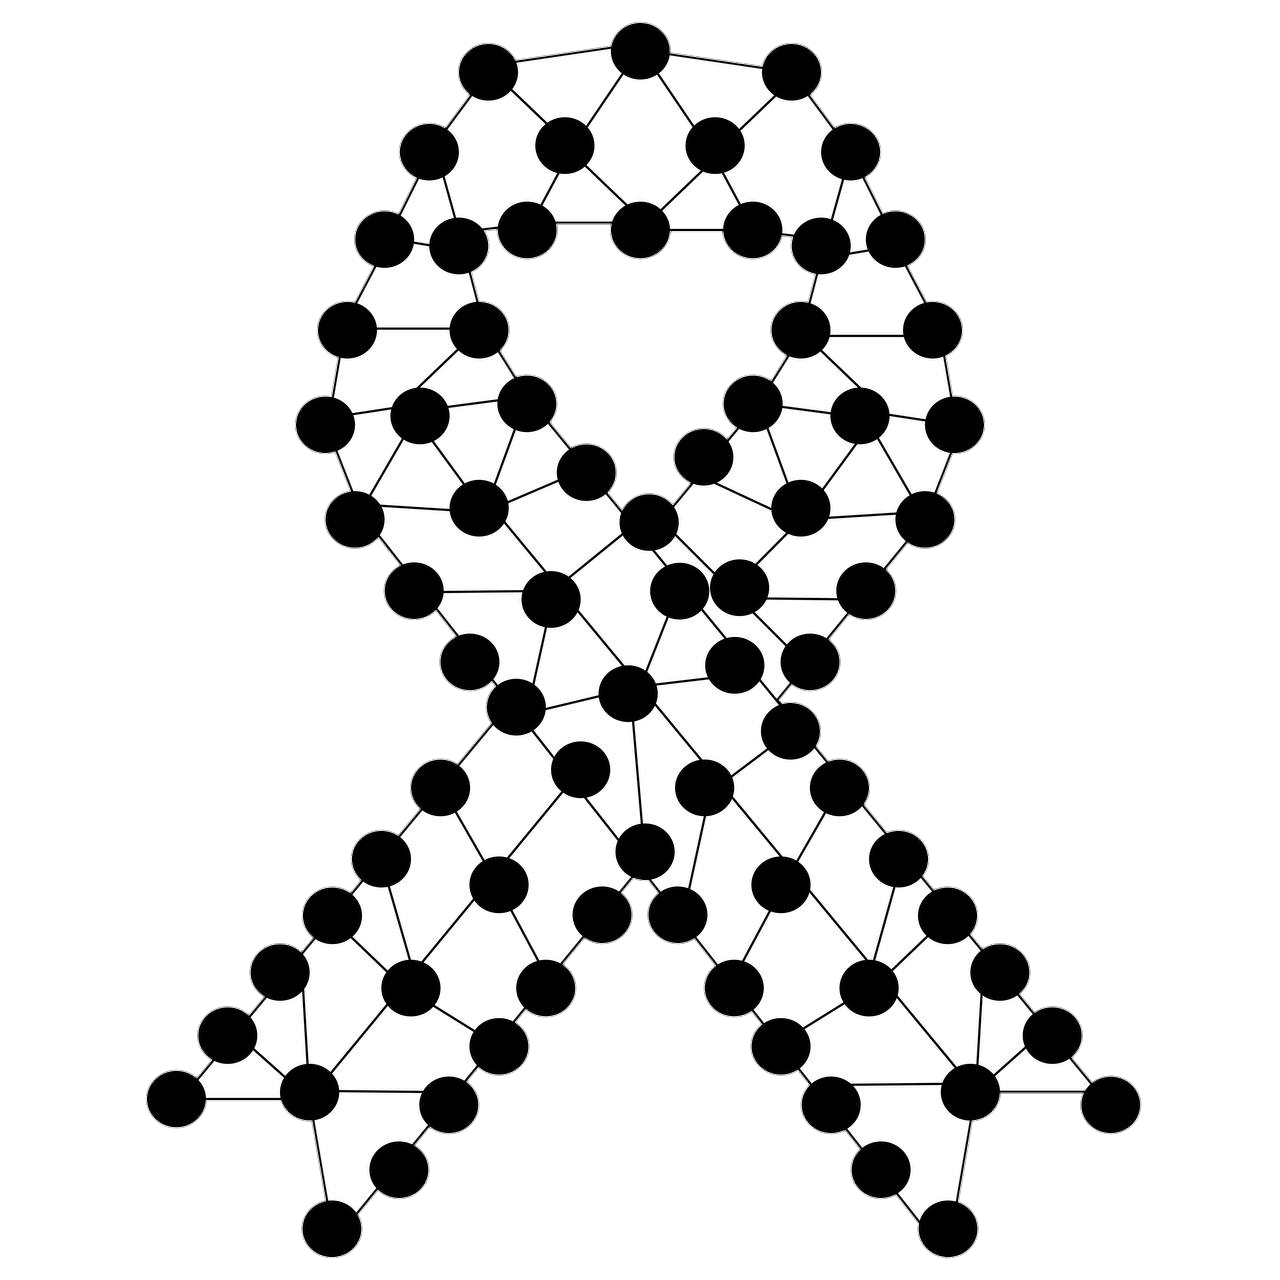
\includegraphics[scale=0.15]{Figures/logo2.0.png}
    \end{figure}
}

\author{Prepared by: \\ 
    Seba Alhejaili \hspace{57pt} 441200901\\
    Fatimah Alhumaidhi \hspace{11pt}  441200921\\
    Lama Almubarak \hspace{33pt}  441200964\\
    Joud Alismail \hspace{57pt}  441201002\\
    Halah Altammami \hspace{25pt}  441201366\\
} 

\supervisor{Dr. Mai Alzamel}

\date{Research project for the degree of Bachelor in Computer Science \\
Second Semester 1444/2023}


\begin{document}

    \cleardoublepage
    \thispagestyle{empty}
    \pagenumbering{gobble}
    \maketitle 

    \newpage
    \pagenumbering{Roman}

    \addcontentsline{toc}{section}{Acknowledgements}
    \section*{\centering  \underline{ACKNOWLEDGMENTS}}
    \hspace{0.7cm} In the name of Allah, the Most Gracious and the Most Merciful, %our deepest gratitude to the people who contributed to the field of Machine Learning in the healthcare sector and made our work applicable to complete. We are grateful to everyone who strives to produce the finest work possible in order to save people's lives.
    our sincere thanks and gratitude to our supervisor, Dr. Mai Alzamel, for her continuous guidance, encouragement, and support throughout our time as her students. We also would like to thank our examiners, Dr. Sarab Almuhaideb, and Dr. Rasha Aleidan, for their invaluable advice and comments on the earlier version of the research. \\

     We are deeply grateful to our parents for their support, prayers, and endless sacrifices to make us reach this step, the end of this research. In appreciation of our siblings, we thank them for the motivation they gave us every time they saw us working. \\

     Finally, we would like to thank our friends and colleagues for their support, understanding, and belief in us.


     \newpage
    \addcontentsline{toc}{section}{English Abstract}
    \section*{English Abstract}
    \hspace{0.7cm} Skin cancer is one of the most dangerous forms of cancer. The more the disease progresses, the more the survival rate steeply decreases. In cases of lethal diseases such as Melanoma, diagnosis in the preliminary stages plays a significant role in determining the probability of getting cured. Nonetheless, the detection of skin cancer in the preliminary stages is an arduous and expensive process. Although this type of cancer is visible to the eye, that does not make it easier to diagnose. People with skin lesions are perplexed because they cannot figure out whether this skin lesion is a cancerous tumor or just a normal lesion. Examining all pigmented skin lesions with surgical treatments causes significant soreness and scarring. Because of that, there is a rising need for an automatic and painless skin cancer detection system with high accuracy. Recently, Machine Learning and Deep Learning have demonstrated promising results in prediction and classification, skin cancer detection had been performed exceptionally well by them. This research tackled the problem of detecting skin cancer by building Deep Learning models that can automatically detect skin cancer using the pre-trained models of Convolutional Neural Network (CNN), namely ResNetv2, VGG16, EfficientNet-B5, and EfficientNet-B7, and comparing them with a Machine Learning model, namely the Support Vector Machine (SVM), in order to determine whether or not the sample is cancerous. The EfficientNet-B7 model with data augmentation outperformed the other presented models with an accuracy of 86.91\%. This document aims to enrich research in the field of skin cancer detection.

    \newpage
    \addcontentsline{toc}{section}{Arabic Abstract}
    \section*{Arabic Abstract}
    \begin{RLtext}
    سرطان الجلد هو أحد أخطر أشكال السرطان. كلما تقدم المرض، انخفض معدل البقاء على قيد الحياة بشكل حاد. في حالات الأمراض الفتاكة مثل سرطان الجلد، يلعب التشخيص في المراحل الأولية دورًا هامًّا في تحديد احتمال الشفاء. ومع ذلك، فإن الكشف عن سرطان الجلد في المراحل الأولية عملية شاقة ومكلفة. على الرغم من أن هذا النوع من السرطان مرئي للعين، إلا أن ذلك لا يسهل التشخيص. يشعر الأشخاص الذين يعانون من الآفات الجلدية بالحيرة لأنهم لا يستطيعون معرفة ما إذا كانت هذه الآفة الجلدية ورما سرطانيا أم مجرد آفة طبيعية. يؤدي فحص جميع الآفات الجلدية المصطبغة بالعلاجات الجراحية إلى وجع وتندب كبيرين. وبسبب ذلك، هناك حاجة متزايدة لنظام الكشف التلقائي وغير المؤلم عن سرطان الجلد بدقة عالية. في الآونة الأخيرة، أظهر التعلم الآلي والتعلم العميق نتائجًا واعدة في التنبؤ والتصنيف، وقد تم إجراء الكشف عن سرطان الجلد بشكل جيد للغاية من قبلهم.
    يتناول البحث مشكلة الكشف عن سرطان الجلد من خلال بناء نماذج التعلم العميق التي يمكنها الكشف تلقائيا عن سرطان الجلد باستخدام المتغيرات المدربة مسبقا للشبكة العصبونية الملتفة \LR{(CNN)}، وهي \LR{ResNetv2}، و \LR{VGG16} و \LR{EfficientNet-B5} و \LR{EfficientNet-B7}، ومقارنتها بنموذج التعلم الآلي، وهو آلة المتجهات الداعمة \LR{(SVM)}، من أجل تحديد ما إذا كانت العينة سرطانية أم لا. إذ تفوق نموذج \LR{EfficientNet-B7} مع نموذج مولد البيانات \LR{(GAN)} على النماذج الأخرى المقدمة بدقة \LR{86.91\%}. 
    سنحاول بإجراء هذا البحث إثراء مجال الكشف عن سرطان الجلد.
    \end{RLtext}
    
    \newpage
    \tableofcontents
    \newpage
    \listoffigures 
    \listoftables 
    \newpage


{\Large \textbf{List of Notations} \par}
\thispagestyle{notations}

\vspace{1cm}


\begin{table}[H]
    \setlength{\tabcolsep}{20pt}
    \renewcommand{\arraystretch}{1.3}
    \large
    \begin{tabular}{l l}

    Adam & Adaptive Moment Estimation \\
    ANN	     & Artificial Neural Network \\
    BGD	 & Batch Gradient Descent \\
    CNN	     & Convolutional neural network \\ 

    \vspace{0.2cm} & \vspace{0.2cm} \\

    DL  	 & Deep Learning \\
    GAN	     & Generative Adversarial Network \\
    HAM10000 & Human Against Machine with 10000 images \\

    \vspace{0.2cm} & \vspace{0.2cm} \\

    ISIC	 & International Skin Imaging Collaboration \\
    KNN	 & K-Nearest Neighbor \\
    MBGD & Mini-Batch Gradient Descent \\
    ML	 & Machine Learning \\

    \vspace{0.2cm} & \vspace{0.2cm} \\
    
    ReLU & Rectified Linear Unit\\
    ResNet	 & Residual Neural Network \\
    SGD	 & Stochastic Gradient Descent \\
    SVM  & Support Vector Machine \\
    Tanh & Hyperbolic Tangent\\

    
    \end{tabular}
\end{table} 

    
    \newpage
    \pagenumbering{Arabic}
    
    \section{Introduction}
    \-\hspace{0.7cm} Skin cancer is a common type of cancer that arises from the skin. The abnormal growth of skin cells causes it to spread, which makes these cells invade other parts of the body \cite{narayanamurthy2018skin}. A number of recent studies have revealed that skin cancer is among the most dangerous types of cancer.  \cite{jain2015computer}. 
    
    Although the skin is an easily accessible site for examination, it is difficult to diagnose skin cancers because many benign lesions visually resemble malignant ones. Consequently, an accurate clinical diagnosis is contingent upon a biopsy and subsequent histopathological examination. Clinicians face the difficulty of determining which and how many skin lesions to biopsisize, typically based on visual inspection and palpation. Despite many efforts, there remains a need for an automated, noninvasive diagnostic method capable of directing biopsies to characterize skin lesions \cite{lieber2009raman}.
   
    As with all types of cancer, it has been demonstrated that screening and preliminary detection of skin cancer is the most reliable indicator of complete recovery \cite{dubal2017skin}. Early detection of skin cancer results in a 94\% ten-year survival rate \cite{dubal2017skin}. Nevertheless, this survival rate plummets as the cancer advances and reaches later stages. When Melanoma, the deadliest form of skin cancer \cite{guy2015vital}, is diagnosed in its final stage, the ten-year survival rate decreases greatly to 15\% \cite{dubal2017skin}. 
   
    With the new technology, it is possible to detect skin cancer at an early stage \cite{jain2015computer}, where it has been shown by different existing systems that computer vision contributes significantly to medical image diagnosis \cite{jain2015computer}. Using machine learning and deep learning, clinicians and patients can streamline diagnostic and therapeutic procedures in a single visit \cite{lieber2009raman}. 
   
    As one of the most threatening forms of cancer, skin cancer detection will be the focus of our research. We will display the performance of the machine learning model, Support Vector Machine (SVM), and the deep learning models, Convolutional Neural Network (CNN), and Convolutional Neural Network with data augmentation using Generative Adversarial Network (GAN). 




    
    \newpage  
    \subsection{Problem Statement}
    \hspace{0.7cm} Skin cancer is regarded as one of the cruelest forms of cancer. Multiple factors, including the high cost of the examination, the pain caused by traditional diagnostic methods, the scarring that occurs during the examination process, and the lengthy process of detecting cancer, discourage patients from undergoing early examination. Early detection of skin cancer saves a great deal of time and effort. It also increases the patient's likelihood of recovery. The development of science and technology has facilitated the discovery and classification of diseases. Using machine learning and deep learning, patients are now able to take photographs of their lesions and send them to a specialist doctor for identification and to initiate treatment. For skin cancer detection, we will in this research develop a machine learning model using SVM, and deep learning model using CNNs and GANs.
    \subsection{Goals and Objectives} \label{section:Goals-and-Objectives}
    \hspace{0.7cm} We intend in our research to build an efficient and robust deep learning model to classify skin lesions into benign and malignant classes. 
    
    \textbf{Objectives:}
    
    In order to achieve our intended goal, the following objectives will be met:
    \begin{itemize}
         \item Reading previous literature on the problem to have a clear view and define the problem's constituents and scope.
         \item Collecting a public dataset of benign/malignant lesions images.
         \item Preprocessing the dataset.
         \item Studying and investigating existing state-of-the-art deep learning classification models in order to choose the most suitable ones to tackle our problem.
         \item Conducting a set of experiments on the chosen dataset.
         \item Implementing the proposed models.
         \item Evaluating our models' performance by conducting multiple performance measurements.
         \item Comparing our results with a machine learning model, which is the Support Vector Machine (SVM).
    \end{itemize}
    
    \newpage
    \subsection{Proposed Solution}
    %  \todo{name what approach of deep learning you are using and why?}
    \hspace{0.7cm} This research seeks to identify skin lesions using Computer-Aided Diagnosis (CAD) systems created using a CNN classifier, as they have proven effective for image classification tasks. We will build our system to take the input image, resize it and remove any noise. The model then segments the input image to separate the lesion from the surrounding skin. Finally, the model will classify the lesion into one of two categories: either benign or malignant. We will train our model using a dataset of images taken from the International Image Collaboration Archive (ISIC) \cite{ISICdataset}. We will use GANs to generate more lesion images in order to overcome any shortage of data. Eventually, the purpose of this research is to develop and train these deep learning models, as well as present measurements that provide a better understanding of the performance of the various approaches on specific medical classification tasks.
    
    \subsection{Research Scope}
    \hspace{0.7cm} Within the framework of deep learning, the primary focus of our research will be on diagnosing skin cancer from images by detecting signs of skin cancer in the images. The model is supposed to show whether a lesion is benign or malignant. Due to the limited number of datasets available for dark skin tones, the scope of our research is limited to light skin tones, and results may not be promising for those with darker skin \cite{rotemberg2021patient}.
    
    \subsection{Research Significance}
    \hspace{0.7cm} In recent years, the field of skin cancer detection using deep learning has developed significantly and is still under development and improvement. The outcome of this study, a model to detect skin cancer using deep learning, will enrich this field and provide numerous benefits. First, the developed models will contribute to reducing the time and effort used to detect skin cancer by surgical methods. Second, it will help to avoid the high cost of detecting skin cancer. Finally, it will increase the rate of early detection due to the ease of detection method and its difference from the painful surgical methods that cause scarring and are usually avoided by patients, which increases the recovery rate.
    
    \subsection{Ethical and Social Implications}
    \hspace{0.7cm} In regards to ethical standards and social implications that we must respect, there is no violation of any of these norms in our research.
    Recent advances in skin cancer detection methods have raised a number of new ethical and legal issues. Usually, these methods require a large number of photos of pigmented moles from many individuals. Consequently, the privacy and confidentiality of data owners could be violated, resulting in ethical issues. 
    In order to protect patients from any potential harm, we selected a publicly published dataset \cite{ISICdataset}, which allowed usage and sharing as long as the source was cited.
    
    \subsection{Report Organization}
    \hspace{0.7cm} The rest of this document is organized into eight chapters. Chapter 2 demonstrates the background including the relevant concepts. Chapter 3 reviews different approaches used in previous works on skin cancer detection. Chapter 4 presents our methodology to tackle the problem. Chapter 5 includes the experimental design. Chapter 6 presents the implementation of our methodology and the limitations and issues that accrued during this phase. Chapter 7 shows the details of the experiments and a discussion of the results. Lastly, chapter 8 concludes the report.

    \newpage
    
    \section{Background}
    \hspace{0.7cm} This chapter demonstrates the techniques, models, and metrics mentioned and/or used throughout this research, including definitions, explanations, and some illustrative examples.
    
    \subsection{Skin Lesion Classification} 
    \hspace{0.7cm} In most cases, skin lesions are harmless. However, some of them may be cancerous. A variety of types of skin cancer exist, including Melanoma, Basal-Cell Carcinoma (BCC), and Squamous-Cell Carcinoma (SCC) that could be benign or malignant \cite{Armstrong2001-ir}\cite{rao1997can}. It is therefore necessary to detect them. Using the ABCD rule can help to detect some malignant lesions. In this rule, the letter 'A' refers to "Asymmetry", which means that the lesion is not of a uniform shape. The letter 'B' represents "Border", which indicates that the borders are not well-defined. Usually, cancerous lesions have more than one color, and the letter 'C' refers to "Color", which indicates the color of the lesion. Finally, the letter 'D' stands for "Diameter", which represents a diameter of more than 6 mm, which is typical for Melanoma lesions \cite{Thanh2020-rw}.
       
    \subsection{Machine Learning} 
    \hspace{0.7cm} Machine learning (ML) is a branch of computer science that was invented in 1959 by Arthur Samuel, who described it as a field of study that enables computers to gather knowledge via experience without the need for explicit programming \cite{Samuel1959-rx}. This term can also refer to the process of solving a practical problem by collecting a dataset and developing a statistical model algorithmically based on that dataset \cite{Burkov2019-rd}. Due to the advent of ML, computers can now perform tasks like classification, clustering, prediction, pattern recognition, etc \cite{Zantalis2019-cl}. Thefour categories of ML algorithms based on their learning technique are: Supervised Learning, Unsupervised Learning, Semi-Supervised Learning, Reinforcement Learning.
   \\ 
   % \textbf{\RomanNumeralCaps { 1. }}  \textbf{Supervised Learning}
   
   %   The first category of ML algorithms is the Supervised Learning algorithm. Generating a target function that predicts class values is the objective of this category. Supervised Learning consists of two phases, the testing phase, and the training phase \cite{Muhammad2015-ip}. The training phase's datasets must have labeled data. The algorithms aim to predict the output values of the testing data by learning the link between the input values and labels. This type of learning is widely used in classification tasks including digit recognition, speech recognition, and identity fraud detection. Additionally, it deals with problems requiring regression, such as weather forecasting, assessing life experience, and population growth prediction, by applying algorithms like Support Vector Machines (SVM), Random Forest, Nearest Neighbor, etc \cite{Zantalis2019-cl}.
   %  \\   
   % \textbf{\RomanNumeralCaps { 2. }}  \textbf{Unsupervised Learning}
    
   %  In Unsupervised Learning, it is not necessary to provide labeled examples. Contrary to Supervised Learning, it is possible to learn from non-labeled examples. It is an algorithm that tries to identify useful properties or patterns in the test data, then identifies groups (clusters) of similar examples and predicts future values based on those clusters. It solves issues related to dimensionality reduction used for visualization of large data sets, detection of hidden structures, and elicitation of features \cite{Kubat2021-rd}.
   %  \\
   %  \textbf{\RomanNumeralCaps { 3. }}  \textbf{Semi-Supervised Learning}
    
   %  In Semi-Supervised Learning, a combination of labeled and unlabeled examples is used to produce an appropriate function or classifier. In this algorithm, the number of examples without labels is commonly greater than the number of examples with labels. The reason is that the large number of unlabeled examples leads to a better model  \cite{Burkov2019-rd}.
   %  \\
   %  \textbf{\RomanNumeralCaps { 4. }}  \textbf{Reinforcement Learning}
    
   %  In Reinforcement Learning, the task is different since the algorithm learns a policy of how to act based on observations of the world \cite{{Burkov2019-rd}}. Instead of learning from a collection of examples that have already been classified, the machine experiments with a system. Then the system responds to this experimentation with rewards or punishments. The system then optimizes its behavior with the goal of increasing rewards while reducing penalties. Reinforcement learning provides solutions to specific types of problems, such as those that need to make decisions sequentially and with a long-term goal, like those in games, robotics, resource management, or logistics \cite{Kubat2021-rd}.

    \subsubsection{Support Vector Machine} 
    \hspace{0.7cm} Support Vector Machine (SVM) is a supervised learning algorithm that was invented by Vapnik and Chervonenkis \cite{Ghosh2019-wm}. Statistical learning theory states that SVM is considered one of the most effective ML algorithms for classification and regression. It has been successfully applied to the recognition of images, categorizing texts, diagnosing medical conditions, remote sensing, and classifying motions \cite{Yuan2010-kh}. This algorithm works according to the principle of margin calculation. Each piece of data is represented as a point in n-dimensional space, and the coordinates of this point are called features. SVM classifies the datasets into classes by trying to find a hyperplane that splits the data as shown in Figure \ref{fig:SVM model}. It works by maximizing the distance between the closest data point in both classes and the hyperplane \cite{Alzubi2018-qf}.
    \begin{figure}[htp]
        \centering
        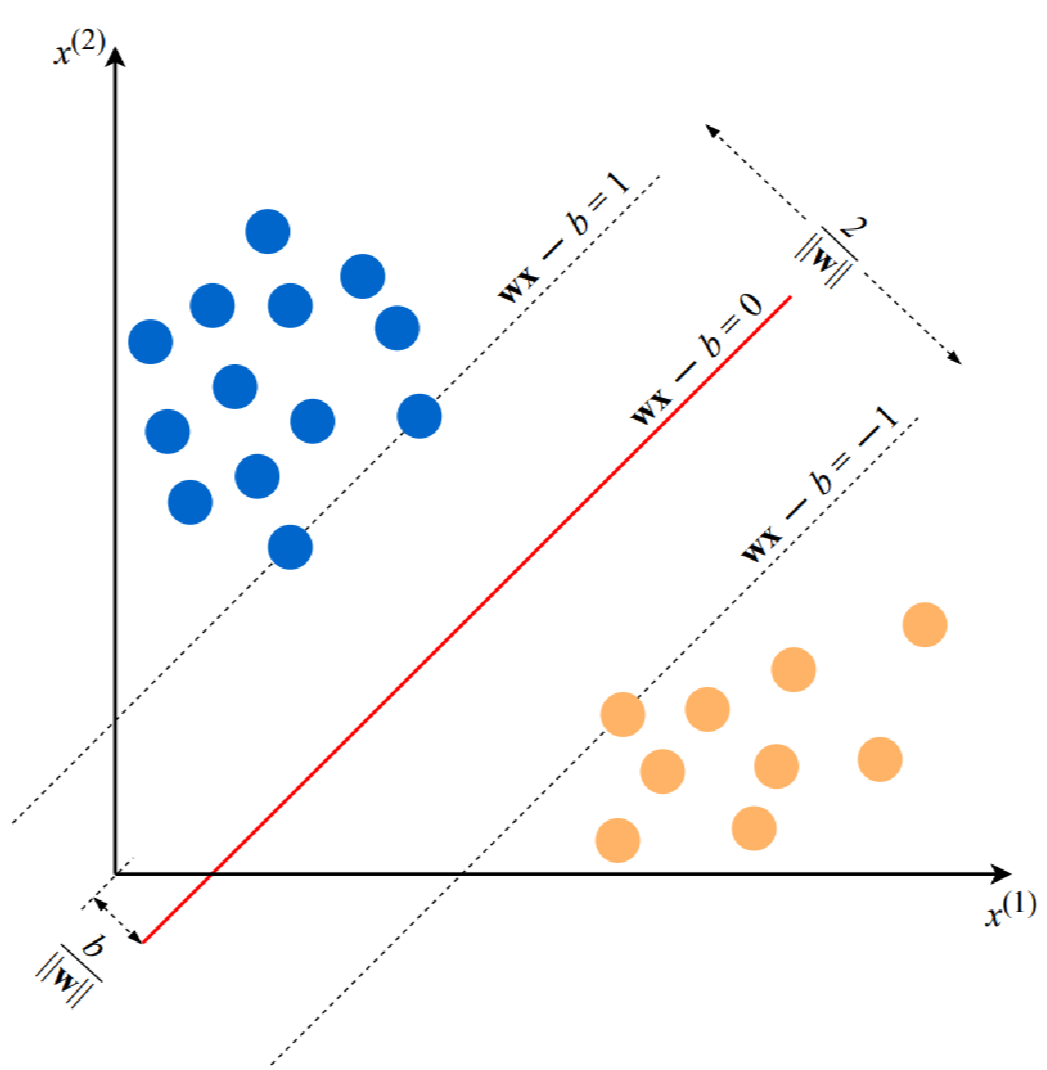
\includegraphics[width=6.5cm]{Figures/SVM example.png}
        \caption[An example of an SVM model for two-dimensional feature vectors]{An example of an SVM model for two-dimensional feature vectors \cite{Burkov2019-rd}.}
        \label{fig:SVM model}
    \end{figure}
        
    % \subsubsection{K-Nearest Neighbor}
    % \hspace{0.7cm} K-Nearest Neighbour (KNN) is a supervised learning algorithm \cite{article}, particularly, it is a classification method for a set of data based on previously classified data learning \cite{wibowo2018k}. In data learning, KNN classifies new data based on its distance from the closest data/neighbors \cite{muliono2020analysis}. As Figure \ref{fig:knn model} illustrates, KNN stores all given prior data (training set) based on a similarity measure, and it uses evidence from nearby sample observations to classify new patterns \cite{singh2019practical}.

    % \begin{figure}[H]
    %     \centering
    %     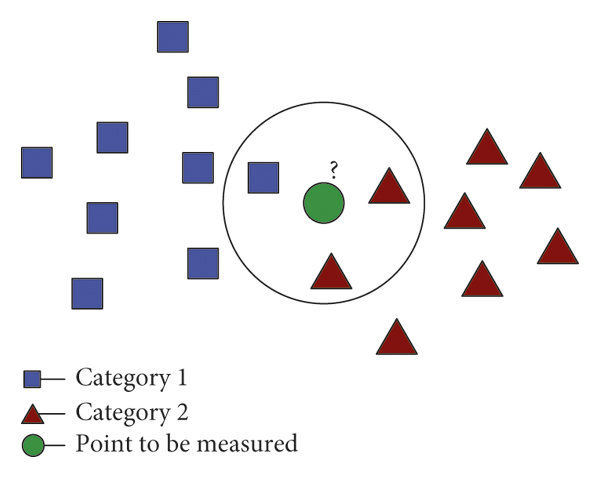
\includegraphics[width=7cm]{Figures/K-nearest-neighbor-algorithm-model.jpg}
    %     \caption[KNN model]{KNN model \cite{zhao2022system}.}
    %     \label{fig:knn model}
    % \end{figure}
        
    % \subsubsection{Decision Trees}
    % \hspace{0.7cm} A typical tree consists of a root, branches, and leaves. The Decision Tree follows the same structure. It is composed of a root node, branches, and leaf nodes. Testing an attribute is performed on each internal node. The result of the test is displayed on the branch, and the class label is displayed on the leaf node. A root node is the parent of all other nodes. A decision tree is a tree in which each node represents a feature (attribute), each link (branch) represents a decision (rule), and each leaf represents an outcome (categorical or continuous value). As decision trees mimic human-level reasoning, it is easy to collect data and make good interpretations. The goal is to create a data tree similar to this one and process a single result at each leaf. Figure \ref{fig:decitree} demonstrates an instance of a decision tree \cite{patel2018study}.
    % \begin{figure}[H]
    %     \centering
    %     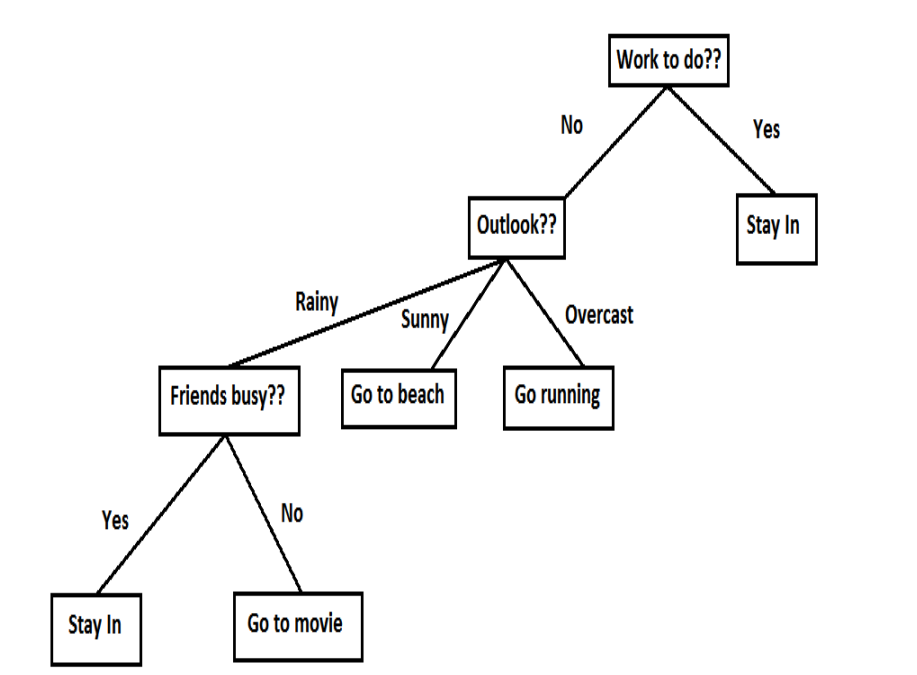
\includegraphics[width=7.7cm]{Figures/decitree.png}
    %     \caption[Example of Decision Tree]{Example of a decision tree on what to do when different situations occur in weather \cite{patel2018study}.}
    %     \label{fig:decitree}
    % \end{figure}

    \subsubsection{Random Forest}
    \hspace{0.7cm} Random Forest is a ML technique that involves training individual classifiers and combining their predictors. It is reserved exclusively for decision tree classifiers and is employed for classification or regression problems. 
    This method generates a set of decision trees from a randomly selected subset of training samples (Figure \ref{fig:Random-Forest}), then regroups the votes from the various decision trees to determine the final class of the test item \cite{azhari2019adaptation}.
    
    \begin{figure}[H]
        \centering
        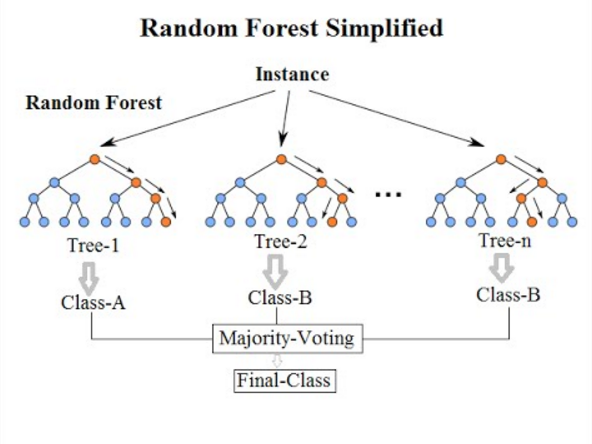
\includegraphics[width=7.7cm]{Figures/Random_forest_diagram_complete.png}
        \caption[Random Forest algorithm mechanism]{Random Forest algorithm mechanism \cite{azhari2019adaptation}.}
        \label{fig:Random-Forest}
    \end{figure}
    
    \subsubsection{Extreme Gradient Boosting Algorithm}
 
    \hspace{0.7cm} Before defining the Extreme Gradient Boosting Algorithm (XGBoost), a related concept, Boosting, must be clarified. Boosting is an ML technique that is applied in classification and regression problems. It generates a weak learner at each step and adds them to the model as a whole. When the direction of the gradient of the loss function is used to determine the weak learner, it is called a Gradient Boosting Machine (GBM). The primary distinction between RF and GBM is that in RF, trees are constructed independently of one another, whereas GBM adds a new tree to complement already constructed trees \cite{pan2018application}. The XGBoost algorithm is a scalable tree-boosting ML system \cite{pan2018application} that is extensively used by data scientists to achieve state-of-the-art results on many challenges \cite{chen2016xgboost}.

    \subsection{Artificial Neural Networks}
    \hspace{0.7cm} An Artificial Neural Network (ANN) is a machine learning method inspired by how biological neural networks work in the brain \cite{Goodfellow-et-al-2016}. The first wave of interest in neural networks (known as Parallel Distributed Processing or Connectionist Models) appeared after the introduction of simplified neurons in 1943 by McCulloch and Pitts \cite{abraham2005artificial}.   ANN is motivated by the enormously distributed parallel computation in the brain, which allows it to be successful at complex control and recognition/classification tasks \cite{hassoun1995fundamentals}.
    The biological neural network that manages those tasks can be mathematically modeled by a weighted, directed graph of greatly interconnected nodes (neurons) \cite{hassoun1995fundamentals}.   
    Commonly, ANNs are structured in layers (Figure \ref{fig:ANNs layers}) composed of interconnected nodes. These nodes contain an activation function.
    The input layer presents a pattern (data) to the network, followed by communication to one or more hidden layers. The actual processing within the hidden layers is done by utilizing a system of weighted connections. Then, the hidden layers are connected to an output layer, where the output is the answer \cite{bartzatt2014determination}. 
    \begin{figure}[H]
        \centering
        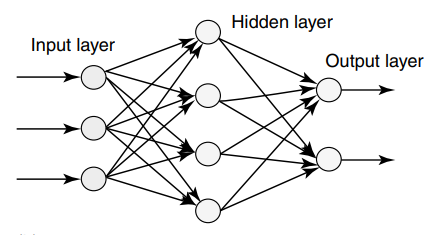
\includegraphics[width=9cm]{Figures/ANN_layers.PNG}
        \caption[Architecture of ANN]{Architecture of ANN \cite{abraham2005artificial}.}
        \label{fig:ANNs layers}
    \end{figure} 
    \hspace{0.3cm}The learning process of an ANN involves updating the connection strength (weight) of a node (neuron) \cite{han2018artificial}.
    One of the ways to ensure lower error rates is by tuning the weights properly because it makes the model reliable and increases its generalization \cite{gnanasekaran2022ground}. An ANN learns based on the difference between predicted and true values, and adjusts its weight, producing a close to true output \cite{han2018artificial}. In neural networks, Back-Propagation is the process of fine-tuning the weights based on error rates \cite{gnanasekaran2022ground}. The name came from the idea of sending information back into the network when the expected output is different from the actual output. 

    \subsubsection{Activation Functions}
    \hspace{0.7cm} Activation Functions are essential in an ANN because it helps in learning and understanding non-linear and complicated mappings between the inputs and corresponding outputs. The prediction accuracy of the neural network is dependent on the number of layers used, and a more critical factor that makes a difference is the
    activation function used. In a neural network, the net inputs are the most important units, which are processed and changed into an output result known as the Unit’s Activation by applying the activation function, also called the Transfer Function or Threshold Function, which is a scalar to scalar transformation \cite{sharma2017activation}.
    
    \subsubsubsection{Sigmoid}
    \hspace{0.7cm} The sigmoid function is a mathematical function commonly used in neural networks trained using back-propagation algorithms for binary classification \cite{sharma2017activation}\cite{jamel2012implementation}. 
    Sigmoid is a non-linear function because its S-shaped curve is limited between 0 and 1 (Figure \ref{fig:sigmoid}), and because it is not symmetric about zero, all output values have the same sign \cite{sharma2017activation} \cite{balaji2013design}.
     While they are not identical, Sigmoid functions are very similar to biological neuron input-output relationships \cite{balaji2013design}. By using it, we provide a limit on the output value of neurons. Here is how the sigmoid function can be expressed:
    \begin{equation*}
        f(x)=\frac{1}{1+ e^{-x}} 
    \end{equation*}
    In this equation, $f(x)$ represents sigmoid activation function, $x$ is the net input value, and $e$ is euler's constant \cite{jamel2012implementation}. 

    \newpage
    \begin{figure}[htp]
        \centering
        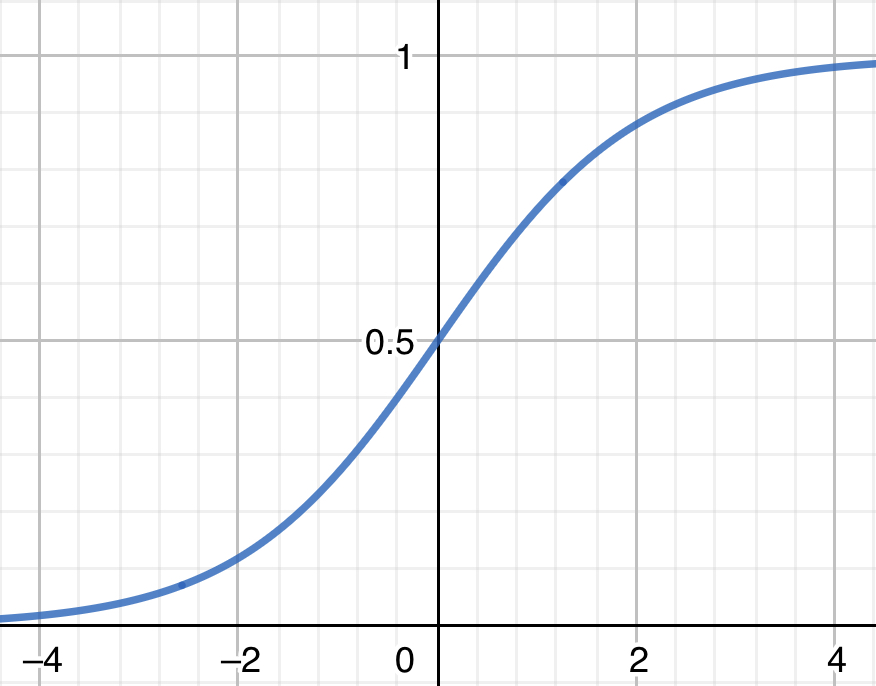
\includegraphics[scale=0.23]{Figures/Sigmoid.jpeg}
        \caption[Sigmoid function plot]{Sigmoid function plot.}
        \label{fig:sigmoid}
    \end{figure}
    
    \subsubsubsection{Hyperbolic Tangent Function}
      \hspace{0.7cm}  The Hyperbolic Tangent Function, also called the Tanh Function, shares a lot of similarities with the Sigmoid function, which is why they are commonly used \cite{sharma2017activation}.
      However, Tanh functions are preferred due to their limit, which lies between -1 and as shown in Figure \ref{fig:tanh}. They also differ in symmetry, as Tanh is symmetric about the origin, resulting in output values with different signs
      \cite{sharma2017activation}\cite{shakiba2020novel}. However, both Tanh and Sigmoid functions are non-linear with S-shaped curves \cite{shamsi2015hyperbolic}. The formula below describes Tanh:
    \begin{equation*}
        f(x) = \frac { e^{x} - e^{-x} } { e^{x} + e^{-x} } 
    \end{equation*} In this case, $f(x)$ is the hyperbolic tangent function of the net input $x$, and $e$ is an euler's constant \cite{shakiba2020novel}.
    
    \begin{figure}[htp]
        \centering
        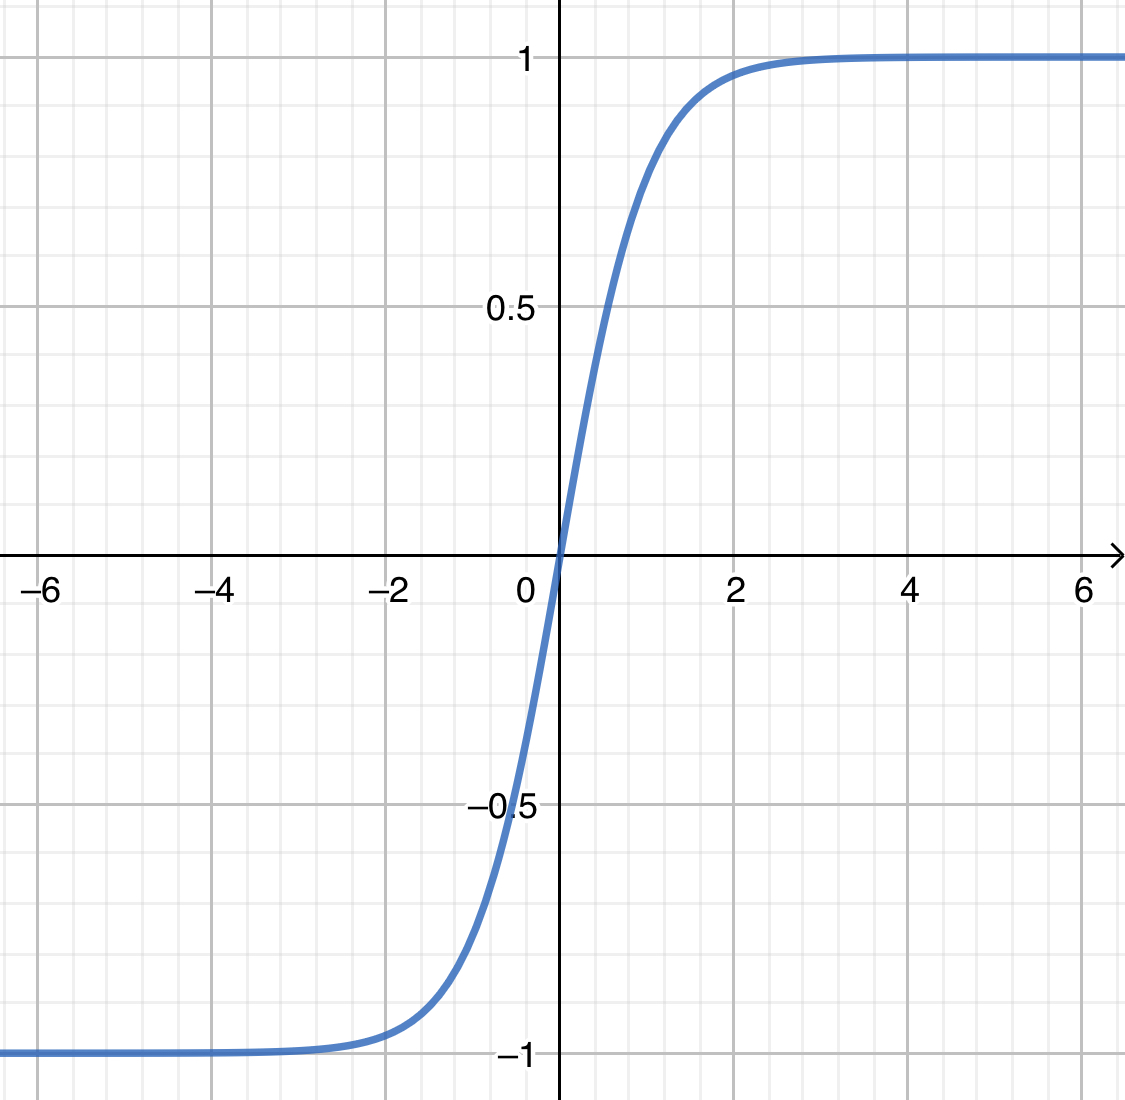
\includegraphics[scale=0.18]{Figures/Tanh.jpeg}
        \caption[Hyperbolic Tangent function plot]{Tanh plot.}
        \label{fig:tanh}
    \end{figure}
    \newpage
    
    \subsubsubsection{Rectified Linear Units Function}
    \hspace{0.7cm} Rectified Linear Units Function (ReLU) is a non-linear activation function \cite{sharma2017activation}. 
    ReLU has become very popular in recent years. It is used to avoid and rectifies the vanishing gradient problem. ReLU is used in hidden layers of ANNs, especially in CNN. Compared to Sigmoid and Tanh, ReLU is less computationally expensive \cite{feng2019performance}. It is defined mathematically as:
    \begin{equation*}
        f(x) = max(0,x)
    \end{equation*}
    \hspace{0.7cm} In the ReLU function, all the neurons are not active simultaneously, making it more efficient than other functions. This means the neuron will deactivate when the output is zero \cite{sharma2017activation}. As illustrated in Figure \ref{fig:relu}, the gradient is 0 for negative inputs, indicating that the weights will not get modified during the descent. The neurons that enter this state will then stop responding to variations in inputs, and they will be stuck forever in an inactive state and "dying"; this is known as the "Dying ReLU" problem \cite{feng2019performance}.
    
    \begin{figure}[H]
        \centering
        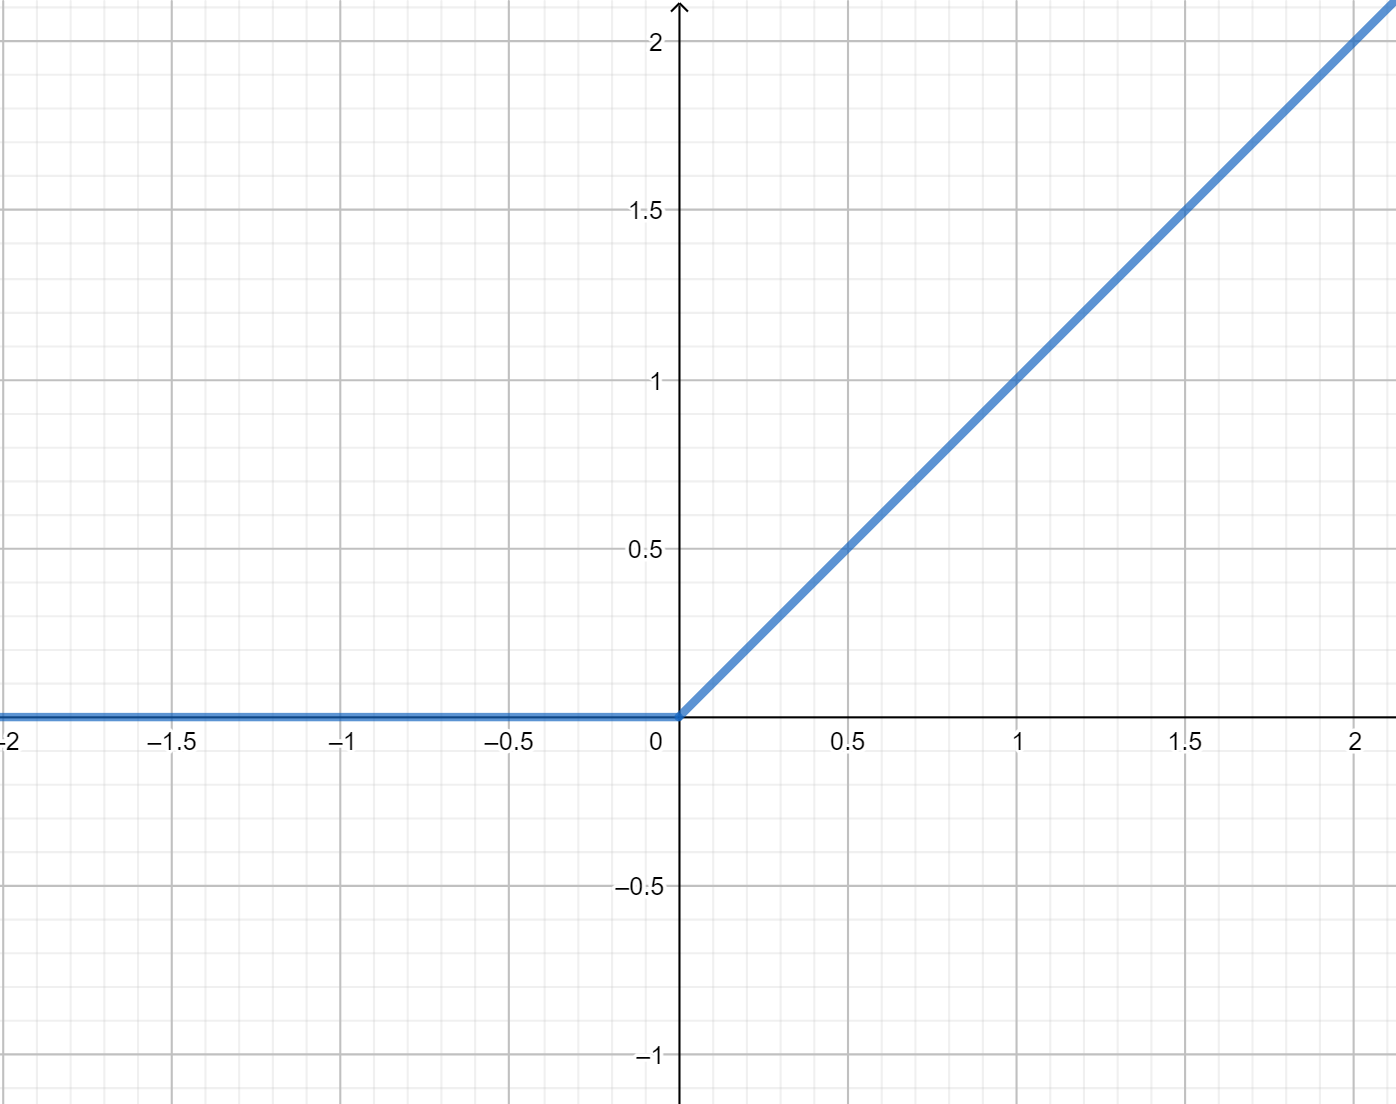
\includegraphics[width=7.5cm]{Figures/relu2.png}
        \caption[Rectified Linear Units function plot]{ReLU plot.}
        \label{fig:relu}
    \end{figure}
    
    % \subsubsubsection{Softmax Function}
    % \hspace{0.7cm} The Softmax Function is a combination of multiple Sigmoid functions. Comparatively to Sigmoid functions which are used for binary classification, Softmax can be used to classify multiclass problems. The Softmax function returns the probability for every data point of all the individual classes. For instance, if we build a network or model for multi-class classification, its output layer will contain as many neurons as the number of classes in the target \cite{sharma2017activation}. It can be expressed as:
    % \begin{equation*}
    %     f(x_{i}) = \frac { e^{x_{i}} } { \sum_{j=1}^{N}  e^{x_{j}} }  (i = 1, 2, ..., N) 
    % \end{equation*}
    
    % The input values of the softmax layer are $x_{1}, x_{2}, ..., x_{N}$, and the output value $f(x_{i})$ represents the probability that the sample belongs to the $i^{th}$ category \cite{wang2018high}.
    
    \subsubsection{Optimization}
    \hspace{0.7cm} The primary objective of ML is to minimize the Cost Function, which is the difference between the predicted output and the actual output. When the cost function is minimized, predictions get closer to the correct answers, which leads to optimization. Optimization is the key component that helps a model to train better during back-propagation by minimizing loss error \cite{gnanasekaran2022ground}. 
    
    \hspace{0.7cm}Recently, several back-propagation optimization algorithms have been used. In this subsection, we will mention some of them.

    \subsubsubsection{Gradient Descent}
    \hspace{0.7cm} Gradient Descent (GD) is an iterative algorithm that is one of the most widely known optimization algorithms and the most common method for optimizing neural networks \cite{ray2019quick} \cite{ruder2016overview}. Its objective is to minimize a cost function. GD is  When the cost function converges to a minimum value, the iterations stop and the cost function is no longer reduced. The approach of GD optimization is used in the Back-propagation algorithm wherein the gradient of the loss function is computed to adjust the weight of neurons. There are three different types of this method, which are: Stochastic Gradient Descent (SGD), Batch Gradient Descent (BGD), and Mini Batch Gradient Descent (MBGD) \cite{ray2019quick}.

    In BGD, the error is computed for every example within the training dataset, but the model will be updated only after completing the evaluation of all the training examples. The main advantage of the BGD algorithm is its efficiency of computation, where it produces a stable convergence and a stable error gradient. Nevertheless, the disadvantage of BGD is that the stable error gradients can sometimes lead to a model that can't achieve its optimal state of convergence. Furthermore, the algorithm requires the entire training dataset to be in memory and available \cite{ray2019quick}. 

    In contrast to BGD, SGD within the dataset calculates the error for each training example, and parameters are updated for each training example. For the specific problem, this could result in SGD being faster than BGD. 
    One of the advantages of SDG is that it provides a detailed rate of improvement due to frequent updates (Figure \ref{fig:stoch}).
    However, frequent updates are more computationally expensive than the BGD method. The frequency of those updates can also produce noisy gradients, causing the error rate to fluctuate instead of decreasing slowly \cite{ray2019quick}. 
    \begin{figure}[H]
        \centering
        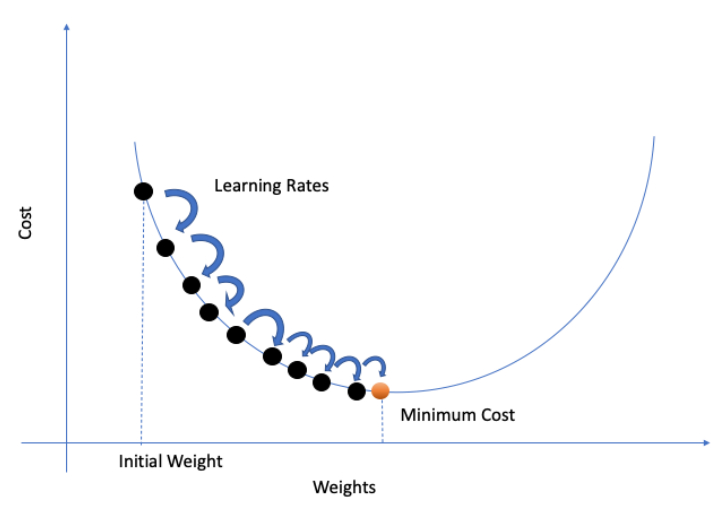
\includegraphics[width=9cm]{Figures/stoch.PNG}
        \caption[Stochastic Gradient Descent]{Stochastic Gradient Descent \cite{ghosh2020empirical}.}
        \label{fig:stoch}
    \end{figure}

    MBGD is obtained by combining the concepts of SGD and BGD. In this approach, the training dataset is split into small batches. For each of the batches, an update is performed. Therefore, it creates a balance between the tenacity of SGD and the effectiveness of BGD. A neural network can be trained with this approach, so it is primarily used in DL \cite{ray2019quick}. 

    % \subsubsubsection{Adaptive Gradient Algorithm}
    % \hspace{0.7cm} Adaptive Gradient Algorithm (AdaGrad) is an optimization algorithm that selects learning based on the situation. Learning rates tend to adapt based on parameters since they are calculated based on certain parameters. As the parameter gradient increases, the learning rate decreases, and vice versa. AdaGrad theory is similar to AdaDelta optimizer. Both measure various learning rates for other parameter elements. Even so, it makes use of gradient squares aggregation. Unlike AdaDelta, AdaGrad uses the gradient squares' moving average \cite{haji2021comparison}.

    % \subsubsubsection{Adaptive Delta} 
    % \hspace{0.7cm} Adaptive Delta (AdaDelta) is an extension of AdaGrad. Instead of accumulating gradients, AdaDelta uses multiple windows of constant size. The algorithm will monitor the gradients available within the window. In the fact of the SGD algorithm requires a learning rate manual selection, selecting an inappropriate learning rate may cause inaccurate predictions. As an enhancement to the SGD algorithm, The adaptive learning rate algorithm (AdaDelta) can adjust the learning rate and improve prediction accuracy automatically \cite{haji2021comparison}.

    \subsubsubsection{Root Mean Square Propagation}
    \hspace{0.7cm} Root Mean Square Propagation (RMSProp) is a well-known algorithm for training adaptive stochastic Deep Neural Networks (DNNs). The gradient is accumulated by the RMSProp algorithm by modifying Adagrad. The average of gradients is exponentially weighted. RMSProp discards historical and retains only current gradient knowledge \cite{haji2021comparison}.

    \subsubsubsection{Adaptive Moment Estimation}
    \hspace{0.7cm} Adaptive Moment Estimation (Adam) is an optimization algorithm of type SGD. For each parameter, Adam calculates adaptable learning rates. In neural networks, there are numerous step-size strategies, but this is one of the most prevalent. The name is a reference to Adaptive Moments. Adam reduces computing costs, requires less memory execution, and is gradient diagonal rescaling invariant \cite{haji2021comparison}. 

    % \subsubsubsection{Nesterov-Accelerated Adaptive Moment Estimation}
    % \hspace{0.7cm} Nesterov-Accelerated Adaptive Moment Estimation (Nadam) is an optimizer created in a similar way to the Adam optimizer, but the idea of this optimizer is that it combines the features of two optimizers: Adam and RMSProp optimizers \cite{haji2021comparison}.

    \subsection{Deep Learning}
    \hspace{0.7cm} Deep learning (DL) uses neural networks with multiple hidden layers; hence the word deep. One of the most significant potentials of DL is its capability of feature representation learning, which contrasts with ML approaches that require tailor-made algorithms to extract features. Based on the available data and the task expected, feature representation learning makes DL networks able to build the right set of features. The result of this ability is that  DL has shown remarkable accuracy in a variety of applications that were previously considered complex or impossible \cite{senthilnathan2022deep}.
    
    \subsubsection{Convolutional Neural Networks} 
    \hspace{0.7cm} A Convolutional Neural Network (CNN) is a deep neural network that has an architecture designed for image analysis that is trained through the process of supervised learning \cite{Haggenmuller2021-hc}. The basic composition of CNN architecture can be divided into five layers, which are: input layer, convolution layer, pooling layer, fully connected layer, and output layer. In the input layer, the input raw dataset will be directly input to the input layer. One image is inputted by its pixel value into the input layer. Convolutional layer  uses a filter to extract features from input and produce a feature map that provides a summary of the features that have been identified in the input \cite{brownlee2019convolutional}. Pooling layer (Down-sampling layer), its main task is to finish the second extraction of the feature data followed by the convolution layer. The fully connected layer is responsible for making all the feature maps connected together as input. This layer integrates and normalizes the abstracted features of the previous convolutions to give a probability for abundant conditions. Eventually, the number of neurons in the output layer is set according to the required conditions. If the classification is required, the number of neurons is generally related to the number of categories to be classified \cite{Gu2019-zo}. CNN uses labeled data such as dermoscopic images with their corresponding diagnoses or ground truths to determine a relationship between the input data and the labels. In such a manner, CNN can apply learned operations to unknown images and classify them using the extracted features \cite{Haggenmuller2021-hc}. Clinical dermatology and dermatopathology diagnoses largely through the recognition of visual patterns. Therefore, using CNN could be helpful in developing additional and/or improved clinically meaningful databases \cite{Tschandl2019-iu}. Figure \ref{fig:Archi} demonstrates the five layers of CNN.
    \begin{figure}[H]
        \centering
        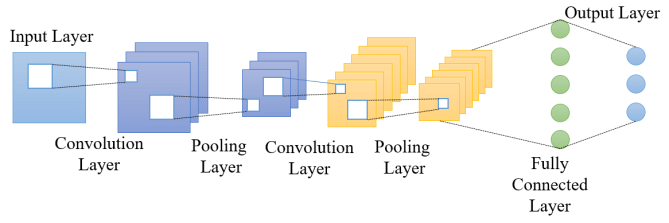
\includegraphics[width=12cm]{Figures/CNN-archi-mybackground.PNG}
        \caption[Basic architecture of CNN]{Basic architecture of CNN \cite{Gu2019-zo}.}
        \label{fig:Archi}
    \end{figure}

    \subsubsection{Residual Neural Networks}
    \hspace{0.7cm} As layers increase in CNN, a problem called the Vanishing/Exploding Gradient occurs. This problem causes the gradient to be zero or too large. Hence, when the number of layers increases, the training and test error rate increases as well \cite{he2016deep}. 
    \begin{figure}[H]
        \centering
        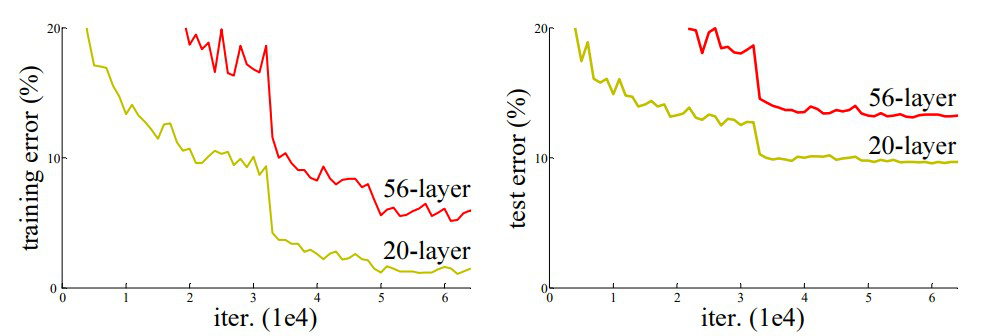
\includegraphics[width=12cm]{CNN_Layers.jpg}
        \caption[Comparison of 20-layer versus 56-layer architecture]{Comparison of 20-layer versus 56-layer architecture \cite{he2016deep}.}
        \label{fig:CNN_Layers}
    \end{figure}
        
    In Figure \ref{fig:CNN_Layers}, it is obvious that a 56-layer CNN gives a higher error rate on both training and testing dataset than a 20-layer CNN architecture. After analyzing more error rates, the authors in \cite{he2016deep} were able to reach the conclusion that it is caused by the vanishing/exploding gradient. A Residual Neural Network (ResNet) was proposed in 2015 by researchers at Microsoft Research for this purpose. To make the problem of the vanishing/exploding gradient solvable, ResNets architecture introduced the concept called Residual Blocks. In this network, a technique called Shortcut Connections (Figure \ref{fig:Residual-Block}) is used. This technique connects activation $\mathcal{F}(x)$ of a layer to further layers by skipping some layers in between, which forms a residual block $\mathcal{H}(x)$. ResNets are made by stacking these residual blocks together. The approach behind this network is that the network fits the residual mapping instead of layers learning the underlying mapping. Thus, instead of saying $\mathcal{H}(x)$, initial mapping, let the network fit: $\mathcal{F}(x) := \mathcal{H}(x) - x$  which gives  $\mathcal{H}(x) := \mathcal{F}(x) + x$. 
    \begin{figure}[htp]
        \centering
        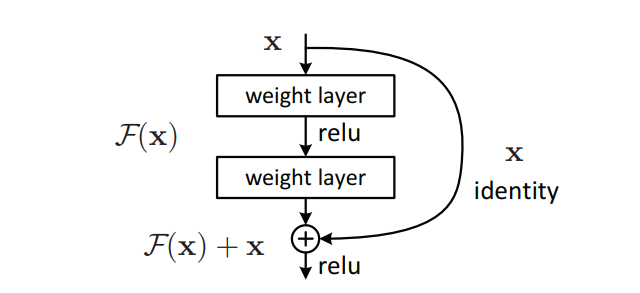
\includegraphics[width=12cm]{Figures/Residual-Block.png}
        \caption[Representation of a  residual block with a shortcut connection]{ Representation of a  residual block with a shortcut connection \cite{he2016deep}.}
        \label{fig:Residual-Block}
    \end{figure}
        
    The idea of using shortcut connections is that if any layer hurt the performance of architecture, then it will be skipped by regularization. In this way, we can train very deep neural networks without the problems caused by vanishing/exploding gradients \cite{he2016deep}.
        
    \subsubsection{Generative Adversarial Networks}
    \label{section: Generative Adversarial Networks}
    \hspace{0.7cm} A network called Generative Adversarial Network (GAN) was first introduced in a 2014 paper by Goodfellow et al. \cite{Goodfellow2014-cu}. GANs are semi-supervised DL models that consist of two parts: a generative model and an adversary model. The generative model generates samples by passing random noise through a multilayer network, which then sends the output to the adversary model. The adversary model is a discriminative model that learns to determine whether a sample is from the model distribution or the data distribution \cite{Goodfellow2014-cu}. Figure \ref{fig:GAN-Structure} shows a high-level visualization of the GAN structure. This framework was based on the two-player minimax game with the following objective function:
    \begin{equation*}
        \begin{aligned}
        \min_{G}\max_{D} V(G,D) = \mathbb{E}_{x\sim pdata(x)}[\log D(x)] + \mathbb{E}_{z\sim pz(z)}[\log (1-D(G(z)))]
        \end{aligned}
     \end{equation*}
   \hspace{0.7cm} In this equation, the generator (G) aims to minimize correct labels for samples from its distribution $z$, while the discriminator (D) strives to maximize the probability of giving the proper label to both training instances $x$ and samples from the generator $G(z)$. GANs showed great success in image generation tasks. One example would be the StyleGAN used in \cite{Karras2019-cc}, which has produced state-of-the-art outcomes for data-driven, unconditional generative image synthesis.
    \begin{figure}[H]
        \centering
        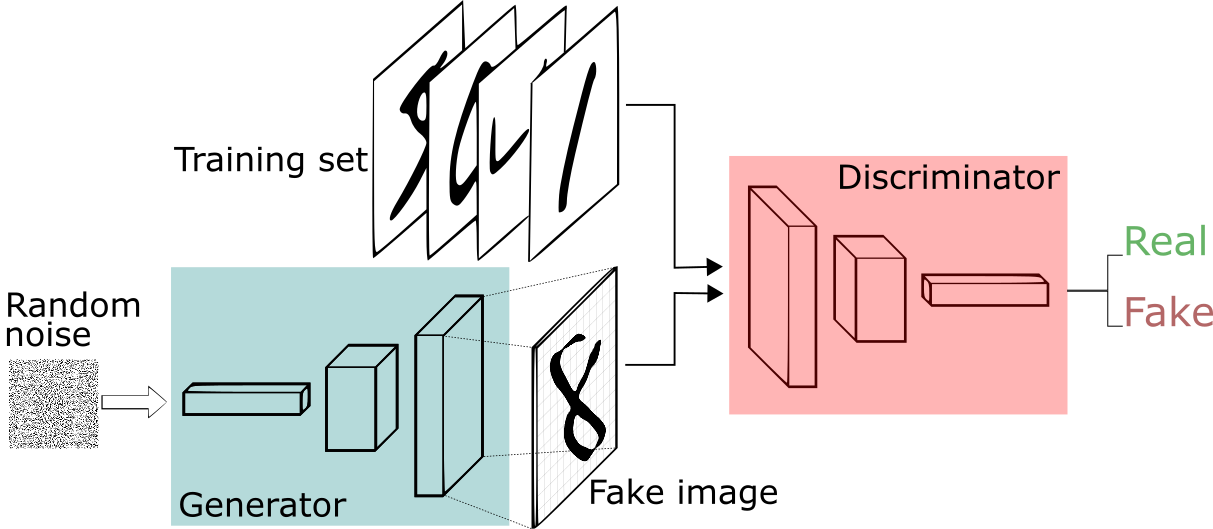
\includegraphics[scale=0.35]{Figures/GANs-structure.jpg}
        \caption[Structure of GAN]{Structure of GAN \cite{silva2017GANs}.}
        \label{fig:GAN-Structure}
    \end{figure}

    \subsubsection{Transfer Learning}
    \hspace{0.7cm} To solve a new task, a human learner is able to transfer relevant knowledge from previous experiences. In contrast, most ML algorithms are designed to address isolated problems. In order to change this, we have to explore the role of Transfer Learning. Through transfer learning, knowledge is transferred from one or more source tasks to improve learning in a related target task \cite{torrey2010transfer}. Figure \ref{fig:Transfer learning} below illustrates some intuitive examples of transfer learning, which are based on the ability of human beings to transfer knowledge across domains. The purpose of transfer learning is to improve performance in a new domain or reduce the required number of labeled examples. \cite{zhuang2020comprehensive}. In general, we will be more successful at mastering a new task if it is closely related to our previous experience \cite{torrey2010transfer}. Besides, the similarities between domains do not always facilitate learning because sometimes the similarities may be misleading \cite{zhuang2020comprehensive}.
    \begin{figure}[htp]
        \centering
        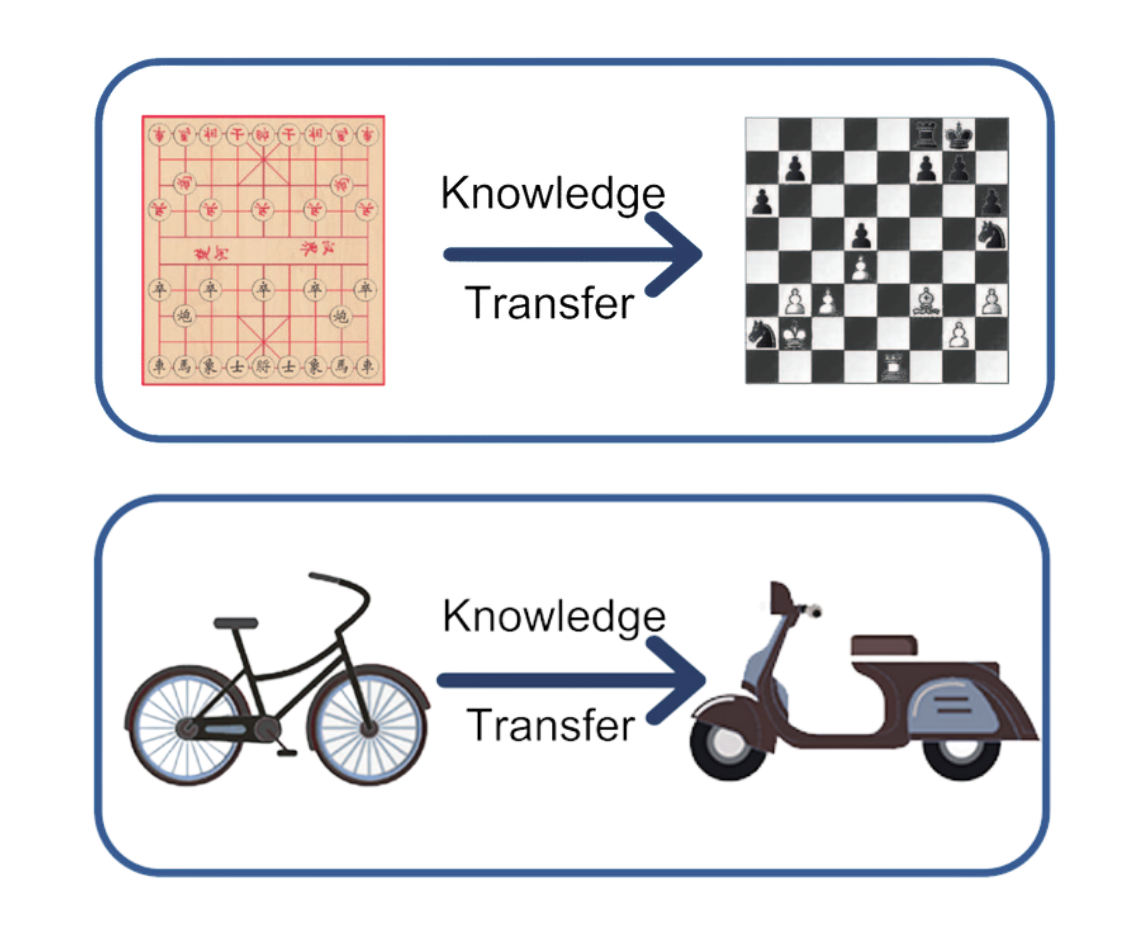
\includegraphics[width=8cm]{Figures/Transfer learning.png}
        \caption[Intuitive examples about transfer learning]{  Intuitive examples about Transfer Learning \cite{zhuang2020comprehensive}. }
        \label{fig:Transfer learning}
    \end{figure}
    \newpage
    There are several examples of transfer learning. In the following, we will demonstrate some of them:
    \\
    \textbf{\RomanNumeralCaps { 1. }}  \textbf{MobileNet}
   
    MobileNet is a lightweight class of Deep Convolutional Neural Networks (DCNNs) with streamlined architectures \cite{ghoury2019real}\cite{howard2017mobilenets}. The size and performance of these networks are vastly superior to those of many other popular models \cite{ghoury2019real}. This technology is used in a variety of fields, including object detection, recognition, mobile, and embedded vision applications \cite{ghoury2019real}\cite{sinha2019thin}. However, it has limited memory, energy, and power limits hardware deployment. Moreover, when the number of parameters and the model size gets reduced, the overall accuracy of the model will decrease \cite{sinha2019thin}.
    \\
    \textbf{\RomanNumeralCaps { 2. }}  \textbf{Inception} 
    
    While scaling up the network, the inception module significantly improves computational efficiency. This module makes excellent use of its internal architecture for two reasons. First, it increases network width and depth to improve overall performance because a bigger size means a larger number of parameters, which causes overfitting in deep networks, leveraging sparsity even within convolutions to perform better results. Therefore filter-level sparsity blocks are introduced in the inception module. Second, reduce input dimensions and eliminate computational bottlenecks \cite{pouyanfar2017efficient}.
    \\
    \textbf{\RomanNumeralCaps { 3. }}  \textbf{Visual Geometry Group} 
    
    Visual Geometry Group, also known as VGG, is a pre-trained CNN model. It was first introduced in a paper titled "Very Deep Convolutional Networks for Large-Scale Image Recognition" \cite{Simonyan2014}. The architecture of VGG is consisting of 16 convolutional layers, each layer has a 3x3 filter size, followed by a pooling layer, a final dense network with two hidden layers, and lastly the output layer \cite{Simonyan2014}. This network was trained on over one million images and gained popularity after it finished first in the ImageNet Challenge in 2014.
    \\
    \textbf{\RomanNumeralCaps { 4. }}  \textbf{EfficientNets}
    
    EfficientNets refer to a family of scaling techniques that uniformly scale all depth/width/resolution dimensions using a simple and highly effective compound coefficient. In scaling up MobileNets and ResNet, EfficientNets demonstrated their efficacy. The creators of EfficientNets achieved considerably higher accuracy and efficiency than previous ConvNets \cite{https://doi.org/10.48550/arxiv.1905.11946}.
    
    \subsection{Image Processing}
    \hspace{0.7cm} An image can be thought of as a two-variable function $f(x, y)$, with $x$ and $y$ being plane coordinates, and the range of $f$ at any given pair of coordinates $(x, y)$ is referred to as the intensity or gray level of the image at that location. Images are considered digital when $x$, $y$, and the range values of $f$ are all finite, discrete quantities with a unique position and value, these components are known as pixels. Digital image processing is the practice of employing a digital computer to process digital pictures \cite{Gonzalez2001-hg}.
    
    \subsubsection{Image Denoising}
    \hspace{0.7cm} Image Denoising is the process of reducing noise in an image. One way of applying denoising techniques is for image smoothing and filtering. An example of image smoothing is the Gaussian Filter, which is defined as follows:
    \begin{equation*}
        \begin{aligned}
            g(x,y) = \frac{1}{\sqrt{2\pi}\sigma}e^{-\frac{d^2}{2\sigma^2}}
        \end{aligned}
    \end{equation*}
    Where $d = \sqrt{(x - x_{c})^2 + (y - y_{c})^2}$ is the distance of the neighborhood pixel $(x, y)$ from the center pixel $(x_{c}, y_{c})$, and $\sigma$ denotes the standard deviation of the distribution, which assumed to have 0 mean \cite{Stockman2001-vr}.
    One intuitive filter named Median Filter is a smoothing filter that uses the median value of a pixel's neighborhood to be replaced by it \cite{Stockman2001-vr}.
    Another filter called Morphological Transformations uses the concept of "Erosion" and "Dilation" to filter noise in images. Erosion and Dilation are two basic morphological operators, the former diminishes the foreground of the object's borders, and the latter dilates it. Other types called Opening (erosion followed by dilation) and Closing (dilation followed by erosion) are also very common \cite{Jain1988-vj}.

    In Figure \ref{fig:Morph}, Ebrahimi et al. \cite{Seyyed_Ebrahimi2010-xg} used Morphological Transformations to detect hair in a lesion image, interpolated hair pixels with neighboring pixels, and applied a median filter for image smoothing.
    \begin{figure}[H]
        \centering
        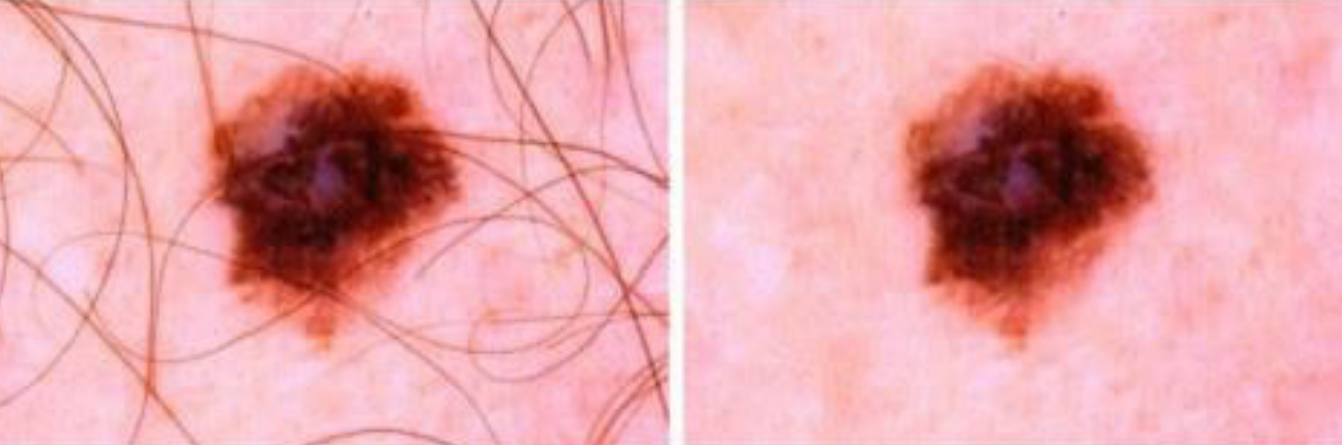
\includegraphics[width=10cm]{Figures/Hair-removal.png}
        \caption[Hair removal from lesion image]{Hair removal from lesion image \cite{Seyyed_Ebrahimi2010-xg}.}
        \label{fig:Morph}
    \end{figure}
    
     \subsubsection{Image Segmentation}
    \label{section: Image segmentation}
    \hspace{0.7cm} Segmentation of an image is the process of separating parts of it into a set of regions in order to represent meaningful areas in it. A region may be defined as a group of pixels with border and shape \cite{Stockman2001-vr}. Some well-known general algorithms for performing segmentation include region growers, clustering algorithms, and edge detectors \cite{Stockman2001-vr}.
    
    A region grower starts at a position in the image, and grows by comparing pixels until they are too dissimilar using some statistical test, one technique proposed by haralick assumes that a region is a set of connected pixels with the same population mean and variance \cite{Stockman2001-vr}.
    
    Clustering is the process of partitioning a set of values into subsets known as Clusters. The process of clustering can be done using algorithms like the iterative K-means method, where K is the number of clusters, or in our case, regions in an image \cite{Stockman2001-vr}.
    
    An intermediate representation for the image region called a Mask can be used for further processing of the segmented image. In this representation, each pixel in the image can be assigned a unique value (or label) representing its region \cite{Stockman2001-vr}. In Figure \ref{fig:segmented-mask}, we can see an instance of a skin lesion image with its mask. The image is segmented into two parts: the lesion and the background. The image was taken from the International Skin Image Collaboration Archive (ISIC) \cite{ISICdataset}.
    \begin{figure}[htp]
        \centering
        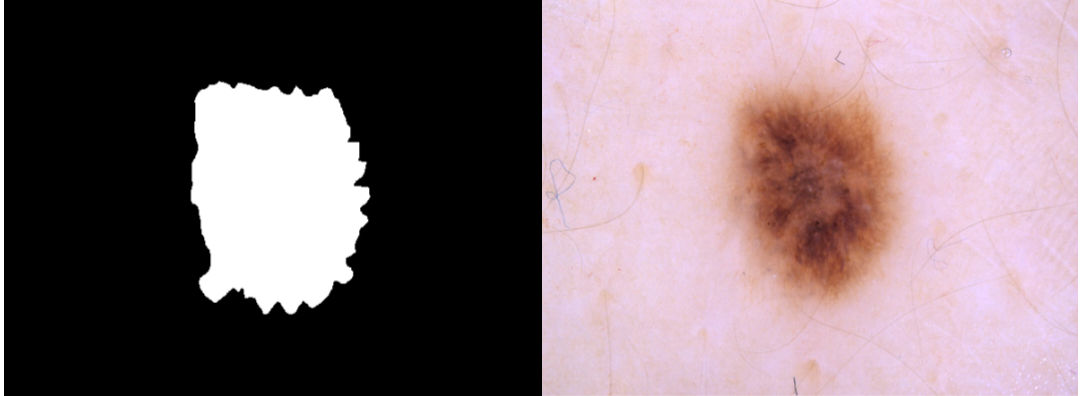
\includegraphics[width=10cm]{Figures/segmented-mask.png}
        \caption[Skin lesion image with its mask]{Skin lesion image with its mask \cite{ISICdataset}.}
        \label{fig:segmented-mask}
    \end{figure}
    \newpage
    \hspace{0.7cm}An example of an effective algorithm to do segmentation, especially for medical purposes, is the U-Net algorithm. It is a neural network architecture designed primarily for image segmentation. A U-Net architecture consists of two paths. First, a contracting path, also known as an encoder or analysis path, provides classification information like a regular convolution network. Second is the expansion path, also called the decoder or the synthesizer. It consists of up-convolutions and concatenations of contracting path features. The creation of highly detailed segmentation maps is what makes U-Net particularly useful in medical imaging. It is also much faster to train U-Net due to its context-based learning capability \cite{siddique2021u}. 
    
    \subsubsection{Color Spaces}
    \hspace{0.7cm} The use of color in image processing is driven by two main reasons. First, color is a strong differentiator that makes identifying and removing objects from a scene easier. Second, compared to merely a few dozen shades of gray, humans can distinguish thousands of distinct color shades \cite{Gonzalez2001-hg}. There are many different color spaces, each of which has a specific color coordinate system. The original theory of Thomas Young (1802) according to which: every color may be represented by combining a suitable selection of three main colors is what gave rise to the development of digital image color representations \cite{Jain1988-vj}.
    
    Red, green, and blue are the three so-called primary colors that the human eye perceives as varying combinations \cite{Gonzalez2001-hg}. These three colors represent the primary spectral components of the RGB model. This model is based on a subspace of a 3-dimensional Cartesian coordinate system. In this subspace, the primary and secondary RGB colors represent three corners of the cube, black represents the origin, and white is the corner farthest from the origin. The grayscale in this system is the subspace centered at the origin (0,0,0), and extended to the white corner (1,1,1) \cite{Gonzalez2001-hg} as seen in Figure \ref{fig:RGB-model}. An RGB system represented by 8-bits has $256^3$ or 16,777,216 color \cite{acharya2005image}.
    \begin{figure}[H]
        \centering
        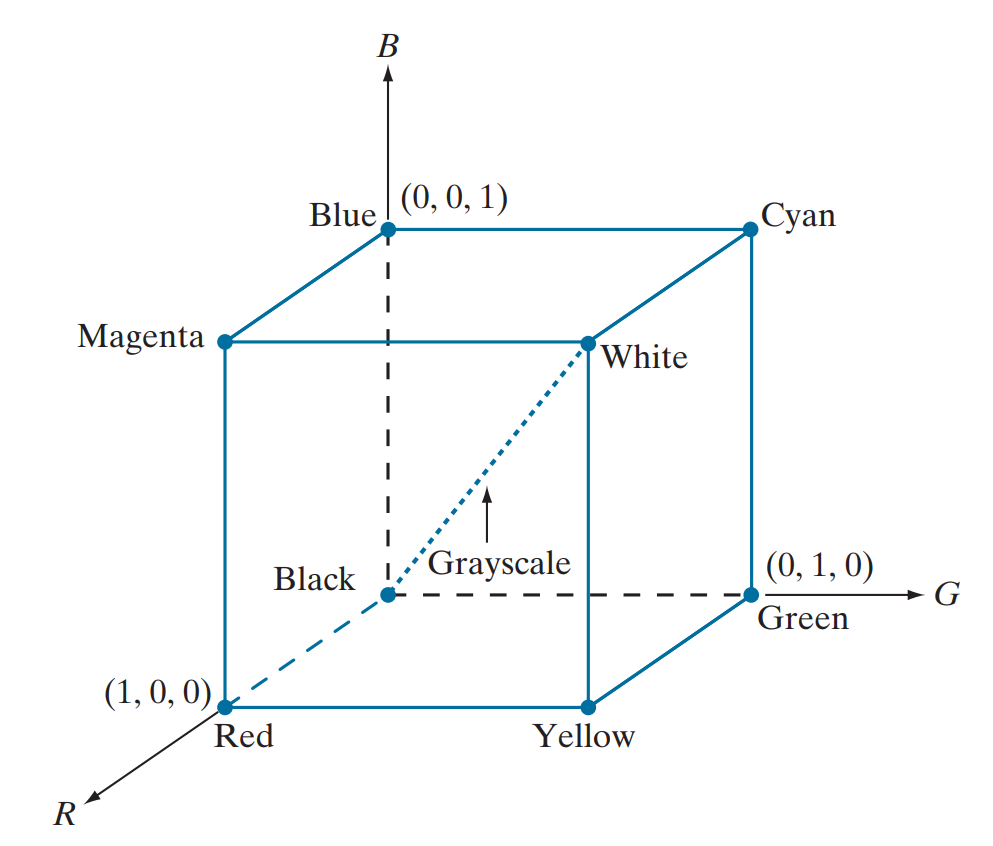
\includegraphics[width=9cm]{Figures/RGB-model.png}
        \caption[Schematic of the RGB color cube]{Schematic of the RGB color cube \cite{Gonzalez2001-hg}.}
        \label{fig:RGB-model}
    \end{figure} 
    
    % As opposed to the RGB model, another model that is the CMY (abbreviation of Cyan, Magenta, and Yellow) subtracts from white instead of adding to black, and so it is referred to as a subtractive model. This is the base model for color printing \cite{Stockman2001-vr}. 
    
    Red, green, and blue values for color description can be difficult for humans to comprehend because we are typically used to expressing colors by values like hue, saturation, and brightness. While saturation indicates how much a pure color has been diluted by white light, hue is a color property that defines a pure color. Brightness is a purely subjective term that is very hard to quantify. It is one of the fundamental elements in expressing color sense. It conveys the achromatic idea of intensity \cite{Gonzalez2001-hg}.  Intensity (gray level) is a greatly helpful term to describe achromatic pictures, which is the reason of being HSI a model that focuses on Hue, Saturation, and Intensity, HSI also can be referred to as HSV using the term "Value" instead of "Intensity" \cite{Stockman2001-vr}. The HSI model benefits from decoupling the color and grayscale data in an image, which makes it appropriate for many of the existing grayscale approaches \cite{Gonzalez2001-hg}.
    
    % The CIE L*a*b* or the CIELAB model is a very popular, device-independent model, meaning its representation stays consistent across screen monitors. This model was introduced by the Commission Internationale de l’Eclairage—the International Commission on Illumination or CIE. Each value in this color system is given by an equation with XYZ values known as the White Tristimulus values, and are defined under the CIE standard D65 illumination. While the L*a*b* gamut includes the whole visible spectrum and may properly represent the colors of any display, print, or input device, the L*a*b* colors are not immediately displayable and must be converted to another color space. The L*a*b* system is helpful in both image processing and image compression applications because, like the HSI system, it is a good decoupler of intensity (represented by lightness L*) and color (represented by a* for red minus green and b* for green minus blue) \cite{Gonzalez2001-hg}.
    
    
    \subsection{Performance Measurements}
    % \todo{but we are doing deeplearning} 
    \hspace{0.7cm} There are many ways to evaluate an algorithm's performance in DL classification based on several different features. Most of the performance measurements focus on the classifier's capability to predict correctly. Table \ref{tab:confusion-matrix} represents the confusion matrix for a binary classifier. It is a table that summarizes how successful the classification model is at predicting examples belonging to various classes. In addition, it can help to determine mistake patterns \cite{Burkov2019-rd}. True Positive (TP) refers to the condition while the data is positive and correctly predicted as positive. False Negative (FN) refers to the situation where the data is positive but incorrectly detected as negative. False Positive (FP) represents the condition where the data is negative but incorrectly detected as positive. Lastly, True Negative (TN) indicates the condition where the data is negative and correctly predicted as negative \cite{fu2020convolutional}.
    
    \begin{table}[H]
    \centering
    \resizebox{0.4\textwidth}{!}{
     \begin{tabular}{c|c|c}
        \hline
           & Positive & Negative \\
        \hline
           Positive &  TP & FN  \\
        \hline
            Negative & FP  &  TN  \\ 
       \hline
     \end{tabular}}
     \caption{Confusion Matrix.}
     \label{tab:confusion-matrix}
    \end{table}

    \textbf{Accuracy} is the ratio of the sample's correct predictions to the total number of predictions. \cite{app11199296}. Moreover, it is a helpful metric when errors in predicting all classes are equally important \cite{Burkov2019-rd}. It is given by:
    
    \begin{equation*}
       \textbf{Accuracy} = \frac{TP + TN}{TP + TN + FP + FN}
    \end{equation*}
    
    \textbf{Precision} and \textbf{Recall} are the most frequently used metrics for assessing a model. The precision determines the number of predicted positive instances correctly classified by the algorithm \cite{app11199296}. It is the ratio of correct positive predictions to the overall number of positive predictions as presented in the equation:
    \begin{equation*}
        \textbf{Precision} = \frac {TP}  {TP + FP} 
    \end{equation*}
 
    \textbf{Recall} is the ratio of correct positive predictions to the overall number of positive examples in the test set \cite{Burkov2019-rd}:
    \begin{equation*}
        \textbf{Recall} = \frac {TP}  {TP + FN}
    \end{equation*}

    As the equation shows, F1 Score represents the harmonic mean of precision and recall. A high value of F-measure indicates that both precision and recall are reasonably high \cite{app11199296}.
    \begin{equation*}
        \textbf{F1 Score} = \frac {2 (Recall * Precision)}  {Recall + Precision}
    \end{equation*}
    
    \newpage    
    \section{Literature Review}
    \hspace{0.7cm} A growing number of studies are being conducted using ML and DL to detect skin cancer in recent years. This chapter aims to provide a summary of some previous works that were studied, to show their models, datasets, techniques, and performance.
    
    A 2019 paper by Al-masni et al. \cite{Al-masni2019-sj} proposed a model for lesion segmentation using a Full-resolution Convolutional Network (FrCN). The segmented images were classified using a Deep Residual Network, namely ResNet-50. The authors used the International Skin Image Collaboration (ISIC) 2017 dataset for training and testing, and used rotation transformation on training data to augment more images. In addition, they used transfer learning and fine-tuning to address the shortcomings of their models. The segmenter model achieved 94.03\% accuracy, while the classifier achieved 81.57\% accuracy, and 0.7575 on the F1 Score. The classifier was compared to two other classifiers that did not use segmentation to demonstrate the superior performance of the model.
    
    Daghrir et al. \cite{Daghrir2020-yt} (2020) used a CNN and two ML classifiers, KNN and SVM to be trained on a set of features describing the borders, texture, and color of a skin lesion. These features represented the ABCD from the ABCDE sign, The paper employed a color enhancement technique known as Gaussian (DOG) for pre-processing and noise reduction in order to remove hair from lesion images, as well as Morphological Active Contours without Edges (MorphACWE) for lesion segmentation. The paper chose 640 lesion images from the ISIC Archive for models' training. The models' accuracy results were 57.3\% for the KNN model, 71.8\% for the SVM model, 85.5\% for the CNN model, and 88.4\% on majority voting.
    
    Sarkar et al. \cite{Sarkar2019-ew} (2019) proposed a Deep Depthwise Separable Residual Convolutional Network model. The model has been trained and validated using a subset of the ISIC dataset, and has been tested on 3 other datasets (PH2, DermIS, and MED-NODE). The authors used multiple pre-processing methods such as image denoising using Non-local Means denoising technique, image enhancement using CLAHE-DWT algorithm, and selecting multiple color channels. The channels selected were RGB color space channels, saturation channel of the HSV color space, b* channel of the CIELAB color space, and finally the inverted grey scale color space channel. The paper demonstrated the model's performance using various kernel sizes, with the best performance being 99.49\% accuracy and a 0.9948 F1 Score on the ISIC dataset using a 4x4 kernel and 4 residual blocks. The authors performed a comparative analysis in the paper.

    
    Garg et al. proposed in \cite{Garg2019-pf} a system using CNNs to identify skin cancer and categorize it. A MNIST HAM-10000 dataset was used for skin cancer images. For the classification task, the authors trained a CNN network to classify the given images in the dataset in their respective classes. Moreover, transfer learning was used as well by applying models such as ResNet and VGG16 to increase the classification accuracy of the images, and to compare the accuracy of the model with that of the proposed DL model. Furthermore, to accomplish the optimization purpose, the authors used Adam optimizer. They found that the ResNet model which is pre-trained in ImageNet dataset could be beneficent, and found that it is the successful classification of cancer lesions in the HAM1000 dataset. Also, they mentioned that learning algorithms such as Random Forest, XGBoost, and SVMs were not very effective for classification tasks, and do not give promising results, where the accuracy of Random Forest was 65.9\%, XGBoost was 65.15\%, and SVM was 65.86\%. On the other hand, their CNN model gave a weighted average precision of 0.88, a weighted recall average of 0.74, and a weighted F1 Score of 0.77. The transfer learning approach applied using VGG model gave an accuracy of 78\%, whereas the ResNet model gave an accuracy of 90.5\%,
    
    In \cite{Nahata2020-mb}, Nataha et al. developed a skin cancer detection CNN model that can classify skin cancer types and detect them early. The model was trained and tested on the state-of-art CNNs, namely Inception V3, ResNet50, VGG16, MobileNet, and InceptionResnet to perform a seven-class classification of the skin lesion images. For the dataset, there were two datasets used to develop their research, which are: ISIC 2018, and ISIC 2019. They combined the two datasets and used them as one dataset. The researchers mentioned that using one metric in a classification problem such as accuracy cannot help in evaluating the complete model efficiency effectively. Hence, they measured the accuracy, precision, recall, F1 Score, and support for every class of skin lesion disease. The results of the average metrics achieved by all final CNNs were as follows. In ResNet, researchers got an accuracy of 85\%, a precision of 0.86, a recall of 0.85, and an F1 Score of 0.85. In MobileNet, researchers got an accuracy of 85\%, a precision of 0.86, a recall of 0.85, an F1 Score of 0.85, and support of 6944. In VGG16, researchers got an accuracy of 87\%, a precision of 0.87, a recall of 0.87, and an F1 Score of 0.87. In Inception V3, researchers got an accuracy of 90\%, a precision of 0.90, a recall of 0.90, and an F1 Score of 0.90. Lastly, in InceptionResnet, researchers got an accuracy of 91\%, a precision of 0.91, a recall of 0.91, and an F1 Score of 0.91.
    
    In \cite{Fuadah2020-os}, Nur Fu'adah et al. built a system that used a CNN with three hidden layers, 3 × 3 filter sizes, and output channels of 16, 32, and 64, respectively, to automatically diagnose skin cancer and benign tumor lesions. The used dataset in this study is an augmentation of the ISIC dataset composed of four classes: Dermatofibroma, Nevus Pigments, Squamous-Cell Carcinoma (SCC), and Melanoma. There were 4,000 images. the authors used 3000 training images and 1000 validation images. These images were trained using the CNN model with several optimization techniques, such as SGD, RMSprop, Adam, and Nadam optimizer with a learning rate of 0.001 and using loss categorical cross-entropy.  Their results showed that the Adam optimizer provides the highest performance, with an accuracy value of 99\%, a loss of 0.0346, and precision, recall, and F1 Score values of 0.91. Moreover, they noted that the proposed model has promising usage as an existing tool for medical personnel.
    
    Albahar et al. proposed a new classification model in \cite{Albahar2019-wf} that used 2-layer CNNs with a novel regularizer technique to classify skin lesions as benign or malignant. For training and validation, they used the ISIC dataset, which contains 23906 images. They divided it into 3 parts, and used 5600 images for the training set and 2400 for the validation set in each part. They achieved an average accuracy of 97.49\%. A regularization technique can be used in many different ways to control the complexity of classifiers. \cite{Albahar2019-wf} proposed a novel regularizer based on the standard deviation of the classifier's weight matrix. They were reducing the complexity by penalizing the dispersion of the weight matrix values. Finding an acceptable value for it was a challenging task since it was a continuous variable that was expensive and time-consuming to reach. Additionally, they demonstrated that their model performed better than existing algorithms and could be applied to assist medical practitioners in classifying skin lesions.
    
    According to \cite{Hasan2019-le}, using five steps, they applied a CNN approach to approximately 23907 images collected from the ISIC archive. The first step was pre-processing the data. The authors saved the pre-processed file as a second step which saves each of the pre-processed images in a record along with their classes. In the third step, they feed the pre-processed data to the CNN. Step four was training their model up to 200 times. Eventually, step five was saving the model for other testing purposes. In the last step, the model is used to predict the images that might contain benign or malignant lesions images. In this research, Hasan et al. \cite{Hasan2019-le} used three layers. The first layer is the input layer on which the data sets are trained. Input layers collect data delivered and add weight to them that goes to hidden layers. Neurons in the hidden layer separate features from the data to find patterns. The pattern is then used to select appropriate classes based on output layers. As a final step, binary classification was used to determine classes 1 and 0. There are no harmful cells in class 0, and there are cancerous cells in class 1. After they applied all their steps, the result with the standard evaluation metrics were 0.84 for recall, 0.8325 for precision, 0.8325 for F1 Score, and 89.5\% for accuracy.
    
    
    Mustafa et al. \cite{Mustafa2017-or} proposed research for skin cancer detection using color space. It is used by experimenting with luminance to improve the visualization for GrabCut segmentation accuracy, by extracting corner and geometric features that are used to train the SVM model. Many research works have been done using image processing and computer vision to detect skin cancer, and in most cases, the ABCDE rule has been applied. In their research, they took advantage of asymmetry and boundary rules (AB) to extract features to identify melanoma. Their first step in pre-processing is to enhance the image by modifying the contrast and brightness (reducing the brightness of the light). The HSV color space is better for image processing. Because it splits color data (Chroma) from intensity or lighting (Luma), the next step is color space transformation (HSV). Afterward, they used the GrabCut technique for Segmentation derived from graph cuts. Then they extracted external pixels, known as recognized backgrounds, while the internal pixels were identified as unknown. They created multivariate Gaussian Mixture Models (GMM) from extracted information to determine if the unknown pixels represent either background or foreground. After that, the segmentation results are used to identify the largest contour to derive its features: Geometric Circularity and Harris Corner Detection. They used an SVM model in the classification to train and predict if an image is positive or negative based on the extracted features. Their result shows that the separation using SVM can find the optimum plane to separate the two classes from the trained samples and predict the testing samples. Their results were 0.80 for Accuracy, 0.8621 for precision, and 0.7143 for recall.
    
    In \cite{Rezaoana2020-bt}, Rozaoana et al. presented a CNN system with three main components: feature extraction, detection, and classification. Over 25,000 images were used in the analysis. By enhancing the output to solve the overfitting problem, a data augmentation technique was used to train CNN just-in-time to avoid distortion and maintain the original consistency of input and output data. Several choices for image augmentation were provided to choose values from different sizes. In this way, the model was able to display images in a variety of ways, which maximized its utility. The convolution, activation, and max-pooling layers were used concurrently in this method (CNN). After that, parallel layers were connected at the function level. Thereafter, the flattened features had two layers of Multi-Layer Perceptrons (MLP), and to prevent overfitting, the number of neurons in each layer was altered. Lastly, the final layer was the layer responsible for classification in addition to the softmax layer. Class activation maps are generated for those layers. The function of the created class is to translate the classification paired to the final convolution layer. Based on a comparison of their results of CNN and other models such as VGG-16, and VGG-19, they determined that CNN is the most reliable model with 79.45\% accuracy, 76.17\% precision, 78.15\% recall, and 76.92\% F1 Score, which has the highest score among the models.
    
    Lack of data is one of the primary factors holding back the development of DL techniques for cancer detection. Sedigh et al. \cite{Sedigh2019-ld} tackled this problem using augmented images to train CNN models. The paper used less than a hundred images from the ISIC Archive to train a GAN for this task. According to \cite{Sedigh2019-ld}, the performance of the CNN algorithm for cancer detection increased by nearly 17\% in terms of accuracy, and the F1 Score showed a growth of 0.2 when using the augmented images for CNN training.


    \begin{table}[H]
      \begin{center}
        \makebox[0cm]{
            \begin{tabular}{>{\RaggedRight\bfseries}m{0.06\linewidth} >{\RaggedRight}m{0.06\linewidth} >{\RaggedRight}m{0.19\linewidth} >{\RaggedRight}m{0.22\linewidth} >{\RaggedRight}m{0.11\linewidth} >{\RaggedRight}m{0.11\linewidth} >{\RaggedRight}m{0.08\linewidth} >{\RaggedRight\arraybackslash}m{0.11\linewidth}} \hline 
            
            \textbf{Ref} & \textbf{Year} & \textbf{Dataset} & \textbf{Model(s)} & \textbf{Accuracy} & \textbf{Precision} & \textbf{Recall} & \textbf{F1 Score}\\ \hline 
              
            \cite{Al-masni2019-sj} & 2019 & ISIC 2017 & ResNet50  & 81.57\% & $\varepsilon$ & $\varepsilon$  & 0.7575 \\ \hline 

            \cite{Daghrir2020-yt} & 2020 & ISIC 2019 &  Ensembling (KNN, SVM, CNN)  & 88.4\% & $\varepsilon$  & $\varepsilon$  & $\varepsilon$ \\ \hline 

            \cite{Sarkar2019-ew} & 2019 & ISIC Archive & Deep Depthwise Separable Residual Convolutional Network & 99.49\% & 0.9965 & 0.9931 & 0.9948 \\ \hline 

            \cite{Garg2019-pf} & 2019 & MNIST HAM10000 
            & ResNet \newline VGG16 \newline Self-made CNN \newline Random Forest \newline XGBoost \newline SVM 
            & 90.5\% \newline 78\%  \newline  $\varepsilon$ \newline 65.9\% \newline 65.15\% \newline 65.86\%
            & $\varepsilon$ \newline $\varepsilon$ \newline 0.88 \newline $\varepsilon$ \newline $\varepsilon$ \newline $\varepsilon$ 
            & $\varepsilon$ \newline $\varepsilon$ \newline 0.74 \newline $\varepsilon$ \newline $\varepsilon$ \newline $\varepsilon$ 
            & $\varepsilon$ \newline $\varepsilon$ \newline 0.77 \newline $\varepsilon$ \newline $\varepsilon$ \newline $\varepsilon$ \\ \hline 

            
            \cite{Nahata2020-mb} & 2020 & HAM10000 \newline ISIC 2019
            & ResNet50 \newline MobileNet \newline VGG16 \newline Inception V3 \newline Inception Resnet
            & 85\% \newline 85\% \newline 87\% \newline 90\% \newline 91\%
            & 0.86 \newline 0.86 \newline 0.87 \newline 0.90 \newline 0.91
            & 0.85 \newline 0.85 \newline 0.87 \newline 0.90 \newline 0.91
            & 0.85 \newline 0.85 \newline 0.87 \newline 0.90 \newline 0.91 \\ \hline 
            
            
            \cite{Fuadah2020-os} & 2020 & ISIC Archive & CNN  & 99\% & 0.91 & 0.91 & 0.91 \\ \hline 
              
            \cite{Albahar2019-wf} & 2022 & ISIC Archive & CNN  & 97.49\% & $\varepsilon$  & $\varepsilon$  & $\varepsilon$ \\ \hline 
              
            \cite{Hasan2019-le} & 2019 & HAM10000 & CNN  & 89.5\% & 0.8325 & 0.84 & 0.8325 \\ \hline 
              
            \cite{Mustafa2017-or} & 2017 & DermQuest & SVM  & 80\% & 0.86 & 0.71 & $\varepsilon$ \\ \hline 
              
            \cite{Rezaoana2020-bt} & 2020 & ISIC 2019 &CNN & 79.45\% & 0.76 & 0.78 & 0.77 \\ \hline
              
            \cite{Sedigh2019-ld} & 2019 & ISIC Archive \& Augmented Images & CNN & 71\% & $\varepsilon$ & $\varepsilon$ & 0.7 \\ \hline
              
            \end{tabular}
        }
      \end{center}
      \caption[Summary of the literature review]{\centering Summary of the literature review. Unmentioned performance metrics were denoted with $\varepsilon$.}
        \label{tab:references}
    \end{table}

    
    \newpage
    \section{Methodology}
    \hspace{0.7cm} After evaluating the related work, the most promising models will be implemented, and a study will be conducted to address the challenge of detecting skin cancer from lesion images. Our analysis has established that CNN and SVM are the most appropriate models for this challenge. To evaluate their performance, we will first preprocess the lesion images, and then we will segment them. After that, we will augment the malignant lesions images using GAN and evaluate the performance of the CNN and the SVM models before and after adding augmented data.
    
    % \hspace{0.7cm}After evaluating the related work, the most promising models will be implemented and a study with the aim of addressing the challenge of detecting skin cancer from lesion images will be conducted. Our analysis has established that CNN and SVM are the most appropriate models for this challenge. To evaluate their performance, we will first compare the CNN model and the SVM model. Subsequently, we will augment the data using GAN and re-evaluate the performance of the models after the addition of augmented data.\vspace{5pt}

  \begin{figure}[H]
        \centering
        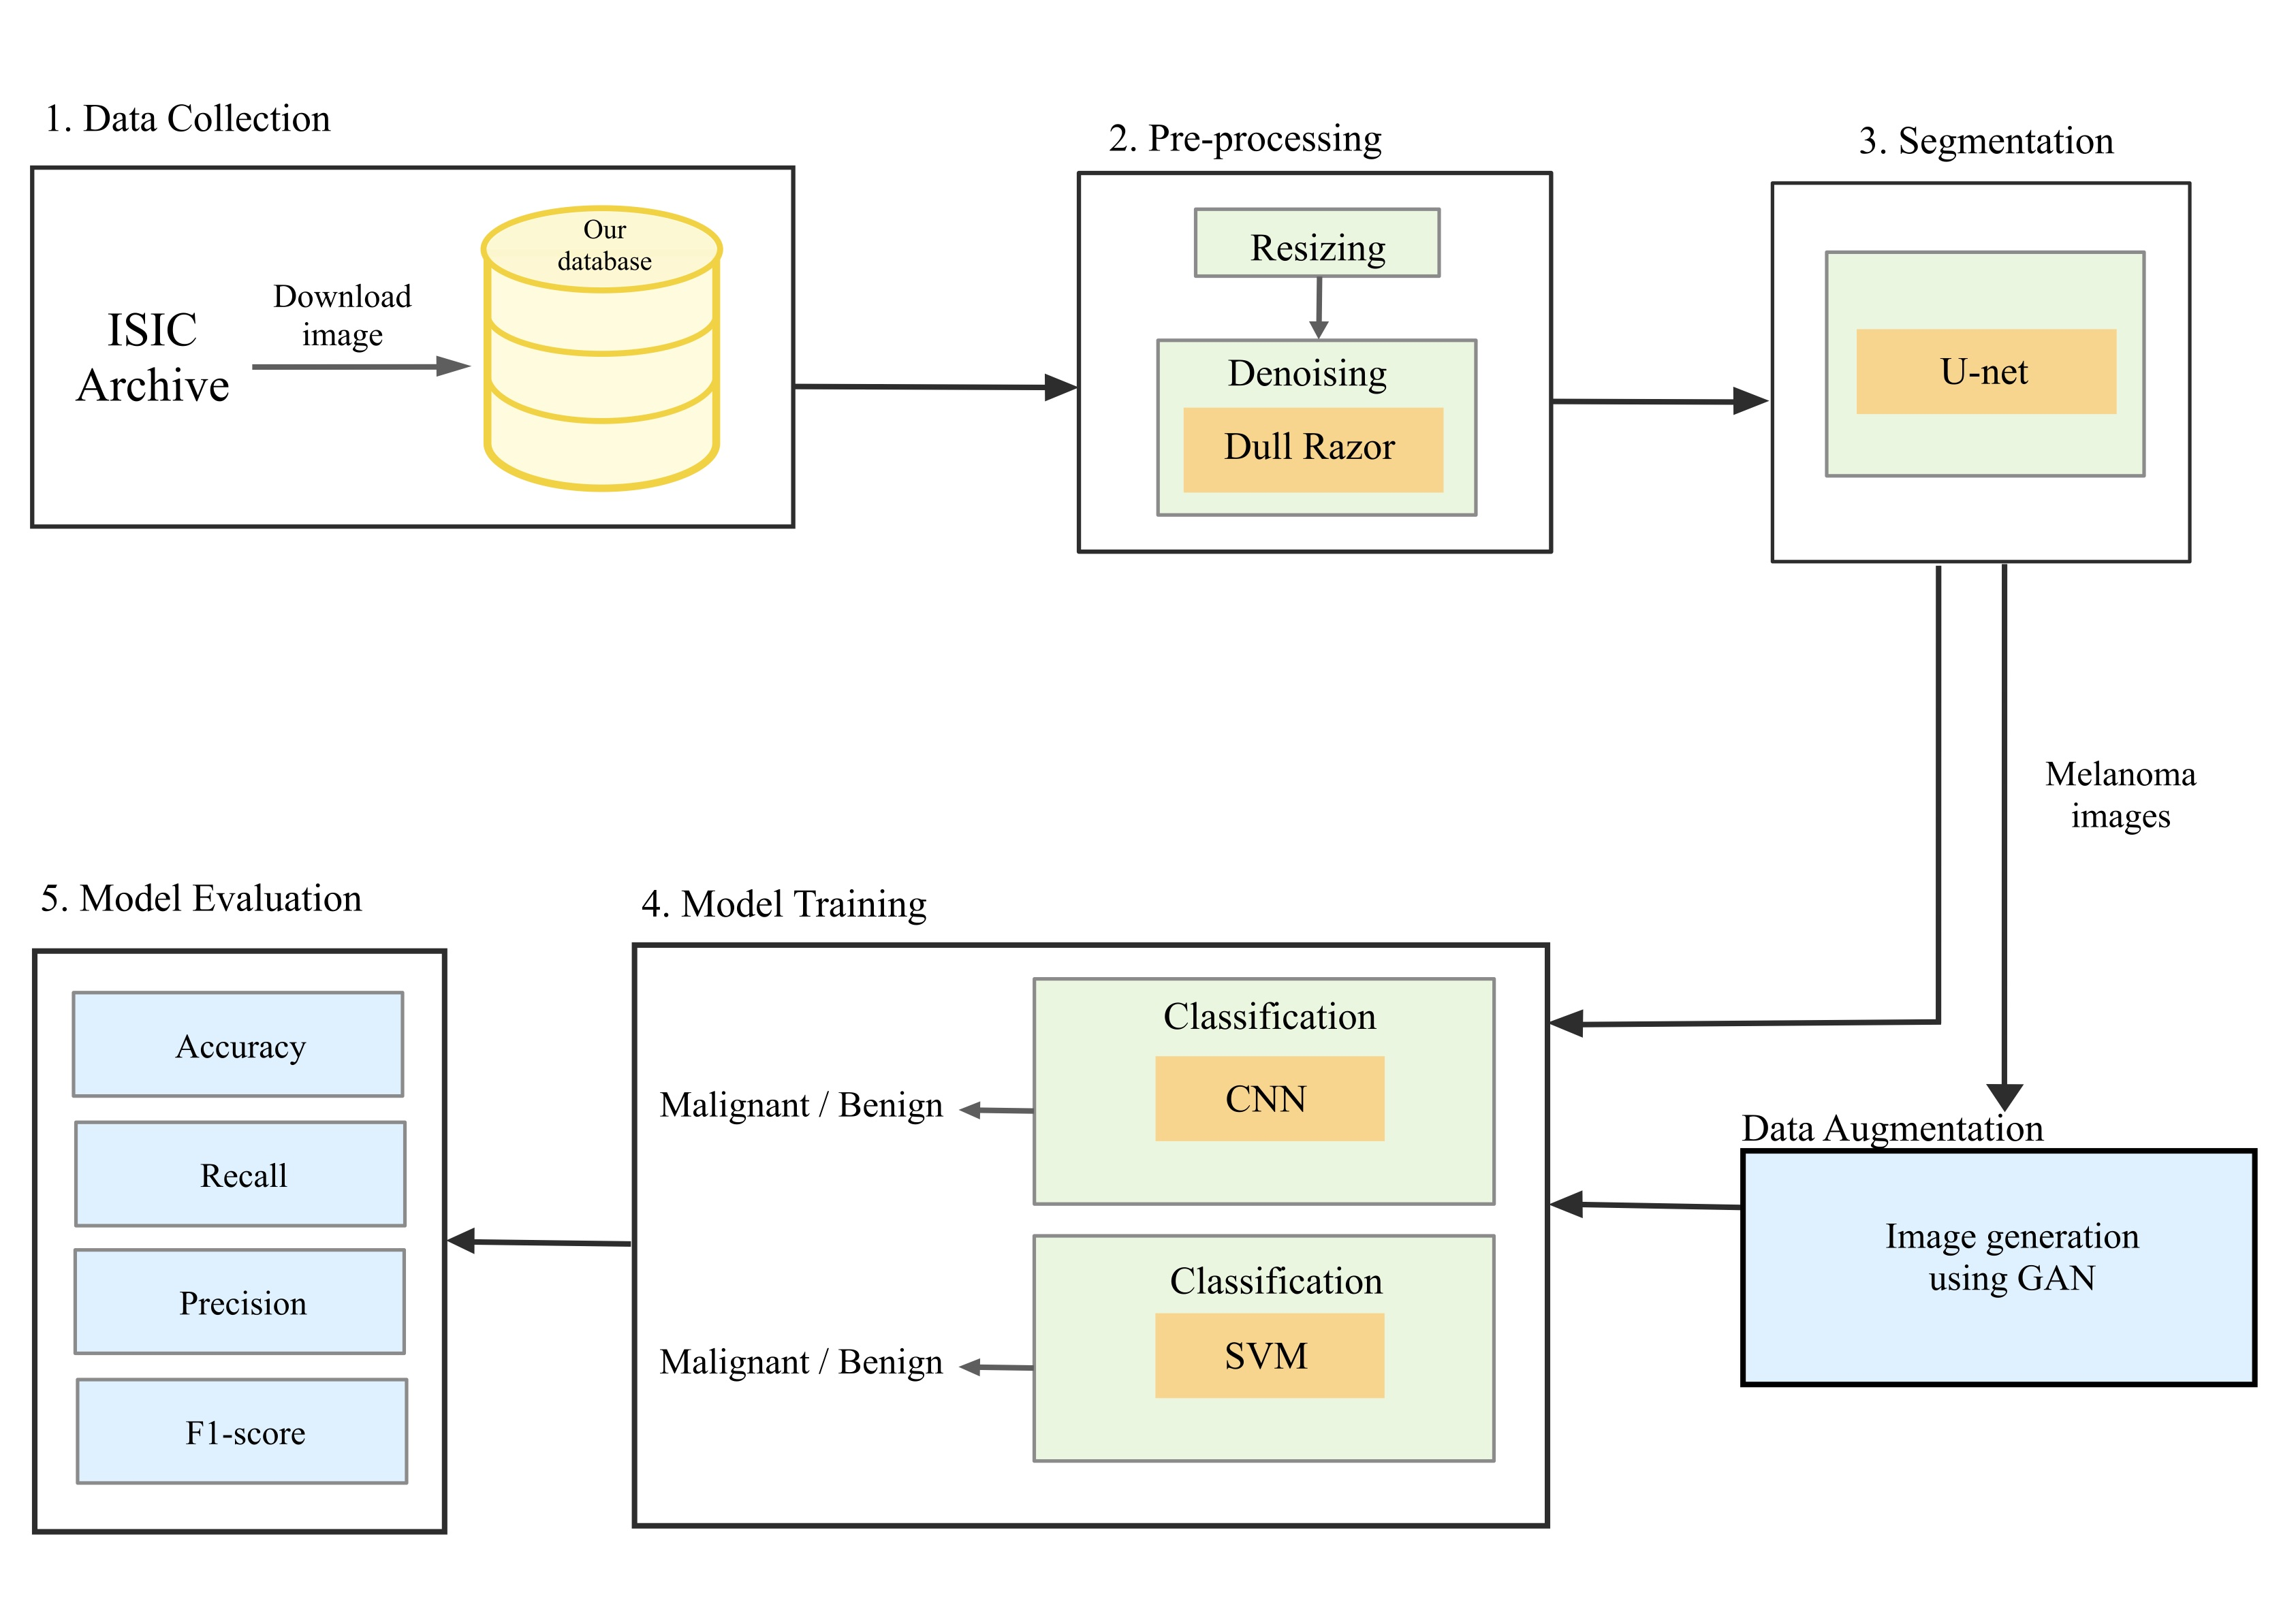
\includegraphics[width=15cm]{Figures/methodology.jpeg}
        \caption[Graphical representation of the metholoogy]{Graphical representation of the metholoogy.}
        \label{fig:Methodology}
    \end{figure}



    \subsection{Preprocessing}
    \-\hspace{0.7cm}In this section, we describe the preprocessing steps we employed in our study to denoise the skin lesion dataset.
    
    \subsubsection{Desnoising}
    \-\hspace{0.7cm} The problem of removing hair from images has been addressed by the development of various algorithms, one of which is the algorithm presented in the work by lee et al. \cite{LEE1997533}. In this research, we introduce the DullRazor algorithm, which is a promising solution to the issue of hair detection and removal.\\

    
    % \textbf{\RomanNumeralCaps { 1. }} \textbf{Data Collection}
    % \\
    % \-\hspace{0.7cm} The International Skin Imaging Collaboration (ISIC) Archive, a dataset of open-source dermoscopy images, will be used to collect skin lesion images with labels and segmented masks \cite{ISICdataset}. In addition, we will generate more malignant lesions images using data augmentation. After evaluating the related work in Table \ref{tab:references}, \cite{Sedigh2019-ld} showed that GANs are suitable for this task, since they showed impressive results in generating realistic images.
    % \\
    

    
    \subsubsection{Segmentation}
    \hspace{0.7cm} Many known techniques tackle the problem of image segmentation, and U-Net will be our choice for this task, since we saw in \ref{section: Image segmentation} that it handles complex structures and shapes, and it is used for medical image segmentation and other tasks where high accuracy is required. Figure \ref{U-Net architecture} below shows a graphical representation of U-Net architecture.
    
    % \-\hspace{0.7cm} There are many known techniques that tackles the problem of image segmentation, U-Net is a deep learning model designed for semantic segmentation tasks in computer vision. It is a fully convolutional neural network (FCN) that is commonly used for medical image segmentation and other tasks where high accuracy is required. The architecture of U-Net is unique, with a symmetrical design that features a contracting path to capture context and a symmetrical expanding path that enables precise localization as seen in Subsection \ref{section:segmentation}. The model combines features from multiple scales and concatenates them with high-resolution activations from the contracting path, allowing for a rich representation of the input image. This combination results in a model that can segment images with high accuracy and handle complex structures and shapes.
    
     % \textbf{\RomanNumeralCaps { 3. }}  \textbf{Data Segmenation}
    % \\
    % \-\hspace{0.7cm} After the data pre-processing stage, data segmentation will be applied. As with the denoising task, segmentation will help at extracting only important information from the image \cite{Gonzalez2001-hg}, Akyel et al. \cite{Akyel2022-vv} mentioned that ineffective noise removal and segmentation are some of the most serious issues that cause inaccuracy in cancer detection models. This means that lesion segmentation is a crucial task to apply before classification, and so, we are concerned with using CNN model for this task.
    % \\
    
      \begin{figure}[H]
        \centering
        \includegraphics[width=16cm]{Architectures figures/U-Net.pdf}
        \caption[U-Net architecture]{U-Net architecture.}
        \label{U-Net architecture}
      \end{figure}

    \subsubsection{Agumentation}
    
    \-\hspace{0.7cm}For data augmentation, we will use GAN, a class of DL models used for image generation and augmentation. They consist of two neural networks, a generator, and a discriminator. The generator creates new images, while the discriminator evaluates the authenticity of the generated images and compares them to the real images in the training dataset, as seen in  \ref{section: Generative Adversarial Networks}. Figure \ref{GAN architecture} shows a graphical representation of the GAN architecture.

   \begin{figure}[H]
        \centering
        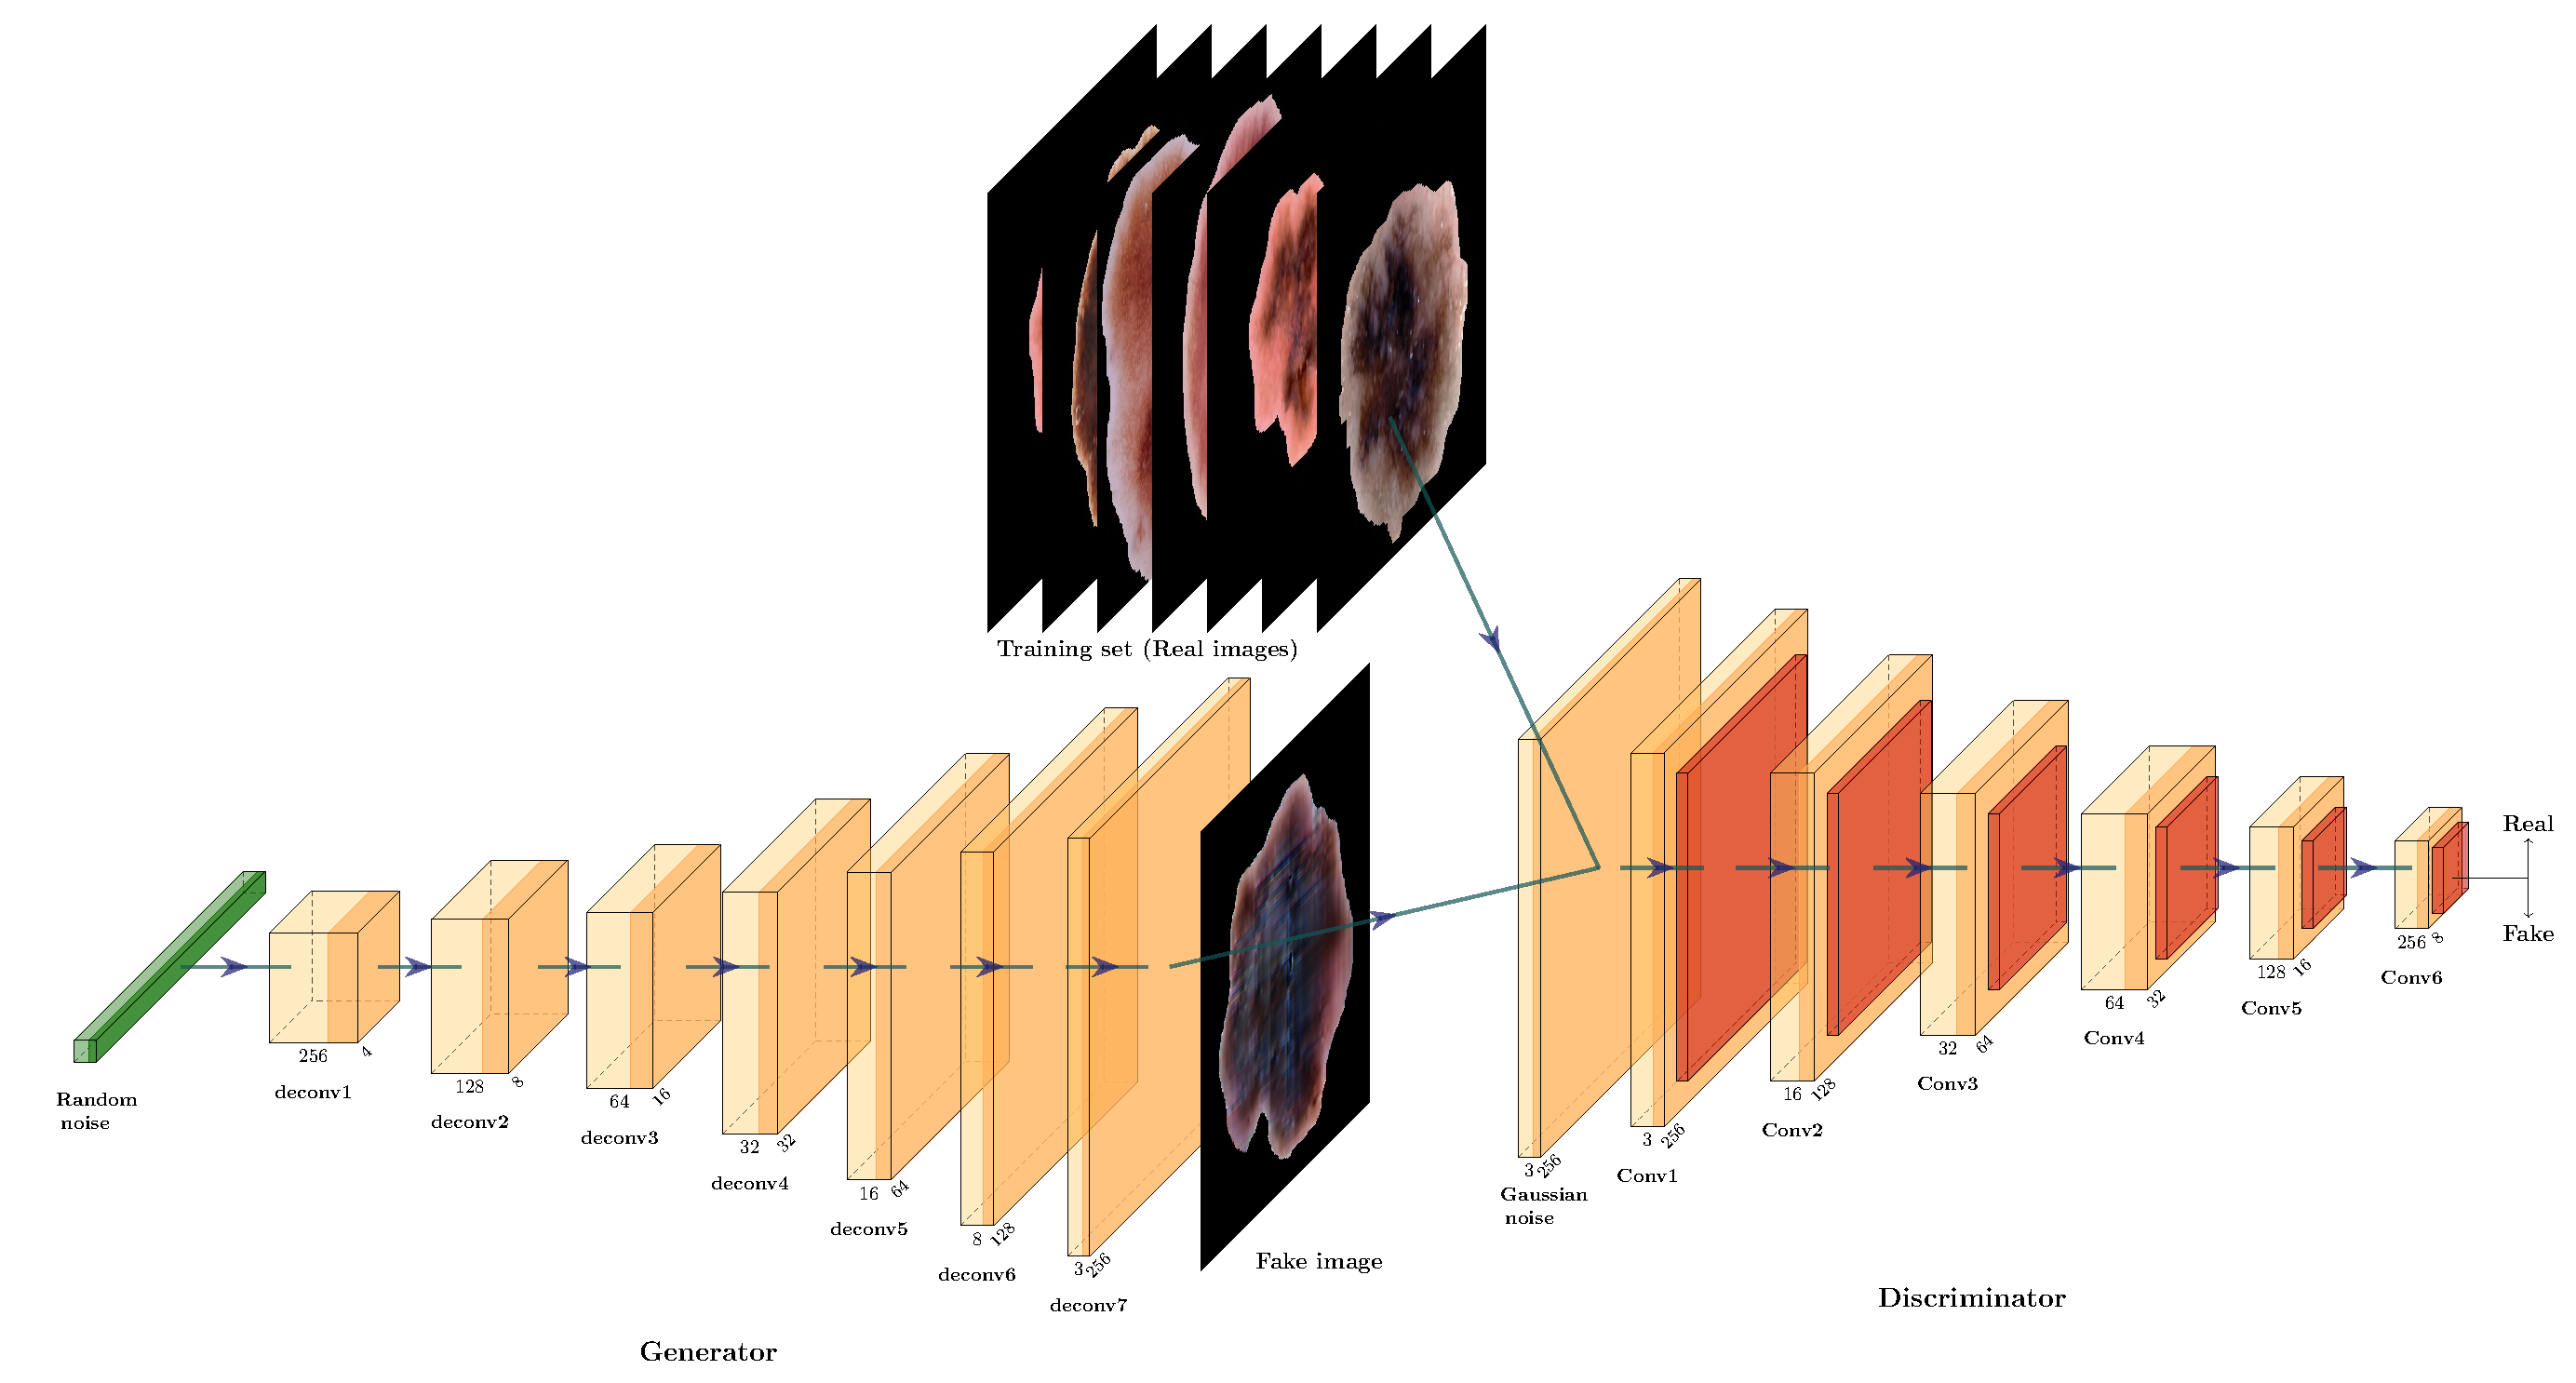
\includegraphics[width=17cm]{Architectures figures/GAN.pdf}
        \caption[GAN architecture]{GAN architecture.}
        \label{GAN architecture}
    \end{figure}
    
    % Generative Adversarial Networks (GANs) are a class of deep learning models that are used for image generation and augmentation. They consist of two neural networks, a generator and a discriminator, that compete against each other. The generator creates new images, while the discriminator evaluates the authenticity of the generated images and compares them to the real images in the training dataset. The goal of the generator is to create images that are indistinguishable from the real images, and the goal of the discriminator is to correctly classify the generated images as fake. The two networks are trained simultaneously, and as the generator improves, the discriminator becomes more challenging, leading to a continuous improvement in the quality of the generated images. GANs have been successfully used for a variety of tasks, including image super-resolution, image style transfer, and image augmentation for improving the performance of computer vision models.
    
 
    

    \subsection{CNN Classifiers}
    \hspace{0.7cm} For the classification task, we will use the following four CNN pre-trained models, which are ResNet50V2, VGG16, EfficientNet-B5, and EfficientNet-B7. These models provide diverse architectures, computational requirements, and performance characteristics, making them suitable for our task. The figures below show the architecture for each pre-trained model, and the tables containing additional final layers for each model.


    
    \subsubsection{ResNet50V02}
         \begin{figure}[H]
            \centering
            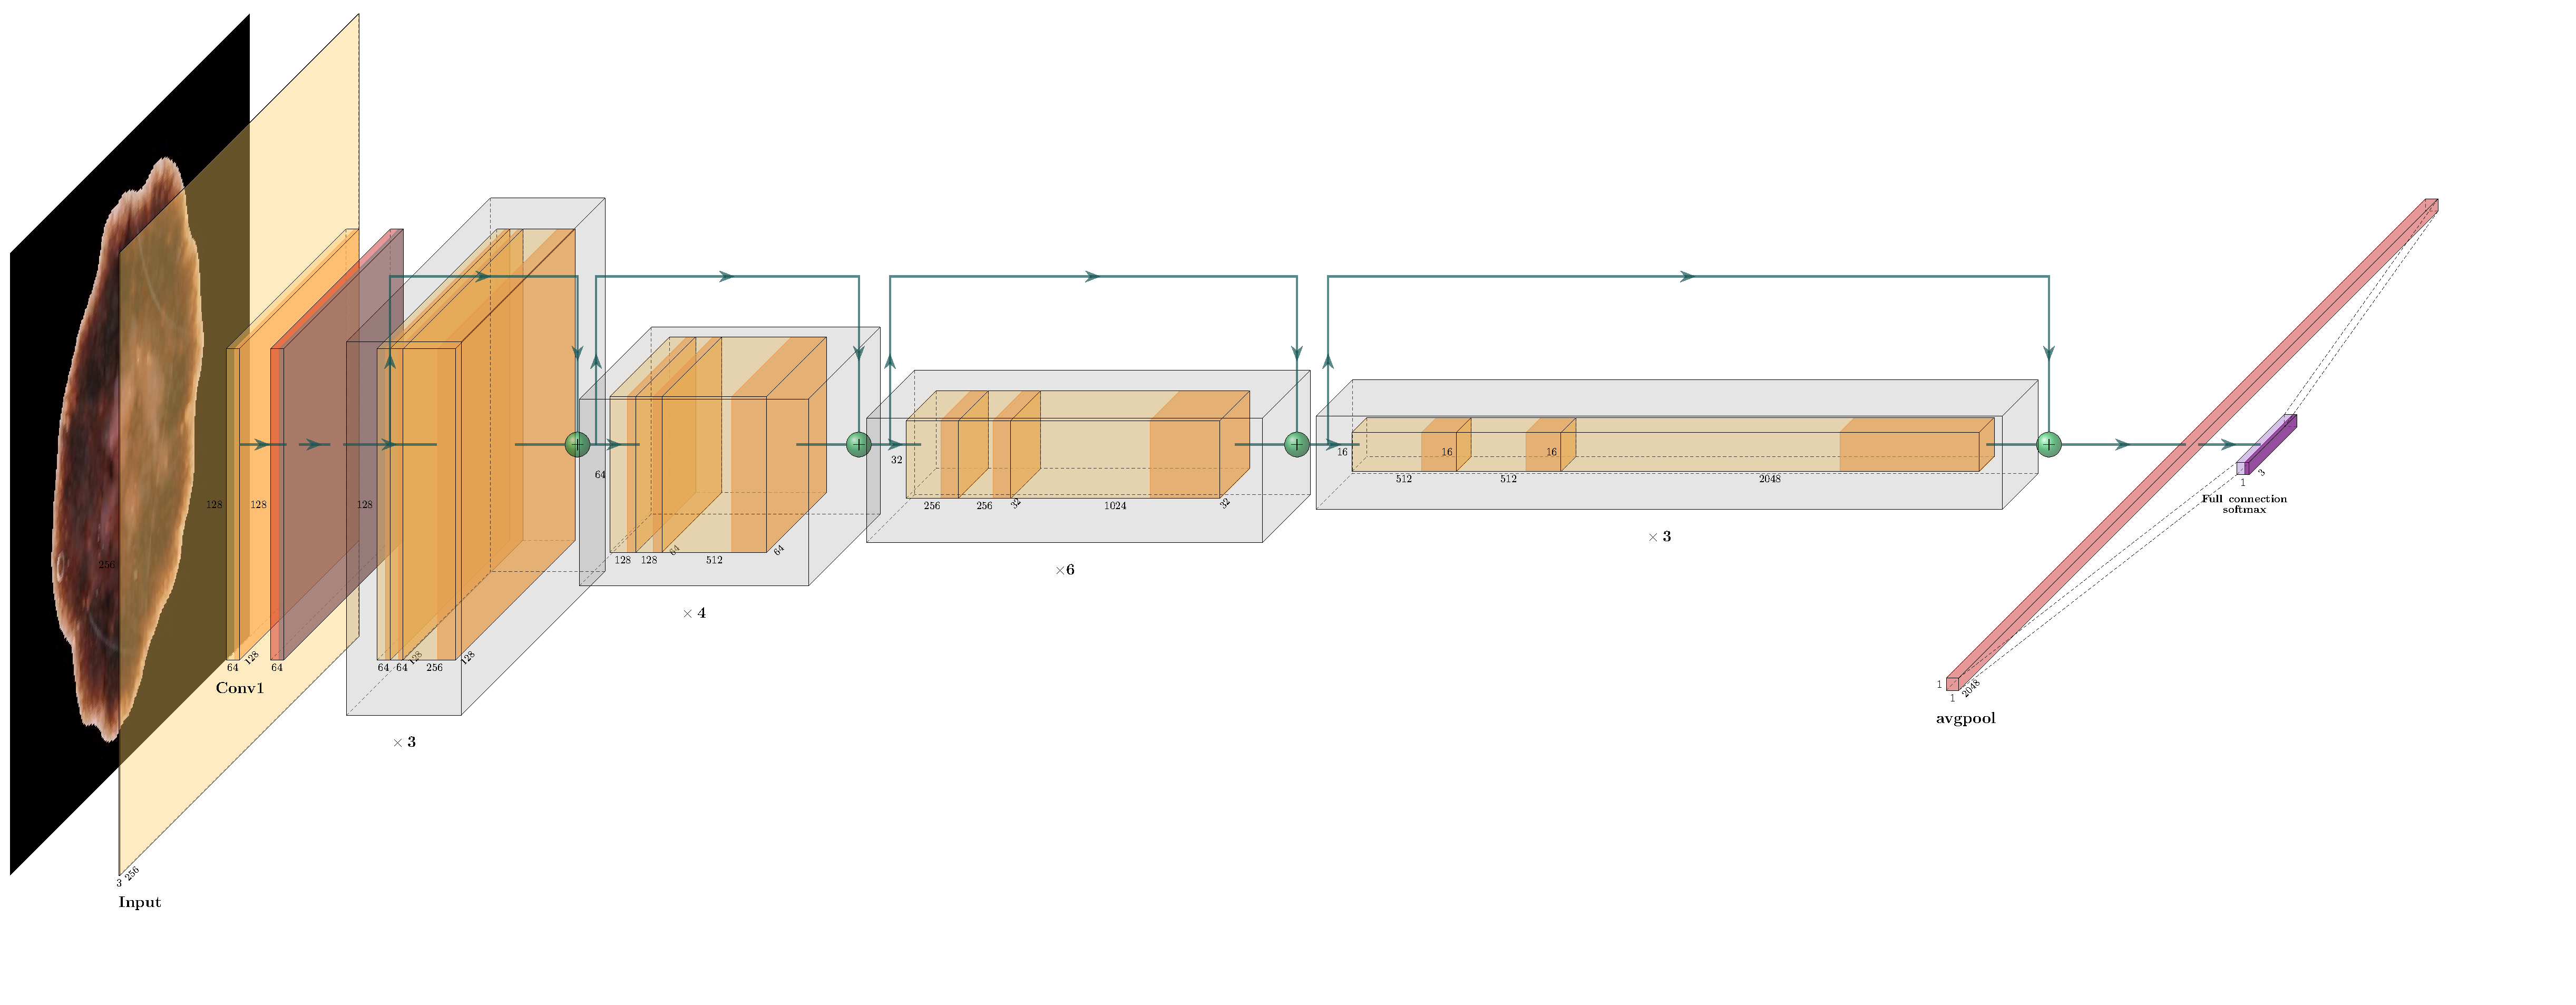
\includegraphics[width=19cm]{Architectures figures/ResNet50.pdf}
            \caption[ResNet50 architecture]{ResNet50V2 architecture.}
        \end{figure}
        \begin{table}[H]
        \begin{center}


        \begin{tabular}{lll}
            \hline
            \textbf{ Layer (type)} & \textbf{Output Shape} & \textbf{Parameter} \\
            \hline
            Input image & (None, 256, 256, 3) & 0 \\
            Resnet50V2 (Functional) & (None, 2048)   & 23564800 \\
            Top flatten (Flatten) & (None, 2048) & 0 \\
            Dense 8 (Dense) & (None, 4096) & 8392704 \\
            Dropout 8 (Dropout) & (None, 4096) & 0 \\
            Dense 9 (Dense)& (None, 32) & 131104\\
            Dropout 9 (Dropout) & (None, 32) & 0\\
            Output layer (Dense)  & (None, 1)  & 33\\
            \hline
        \end{tabular}
        \end{center}
        \caption[Details of ResNet50V2 Model Proposed]{\centering Details of ResNet50V2 model proposed.}
    \end{table}


     
    \subsubsection{VGG16}
    
    \begin{figure}[H]
        \centering
        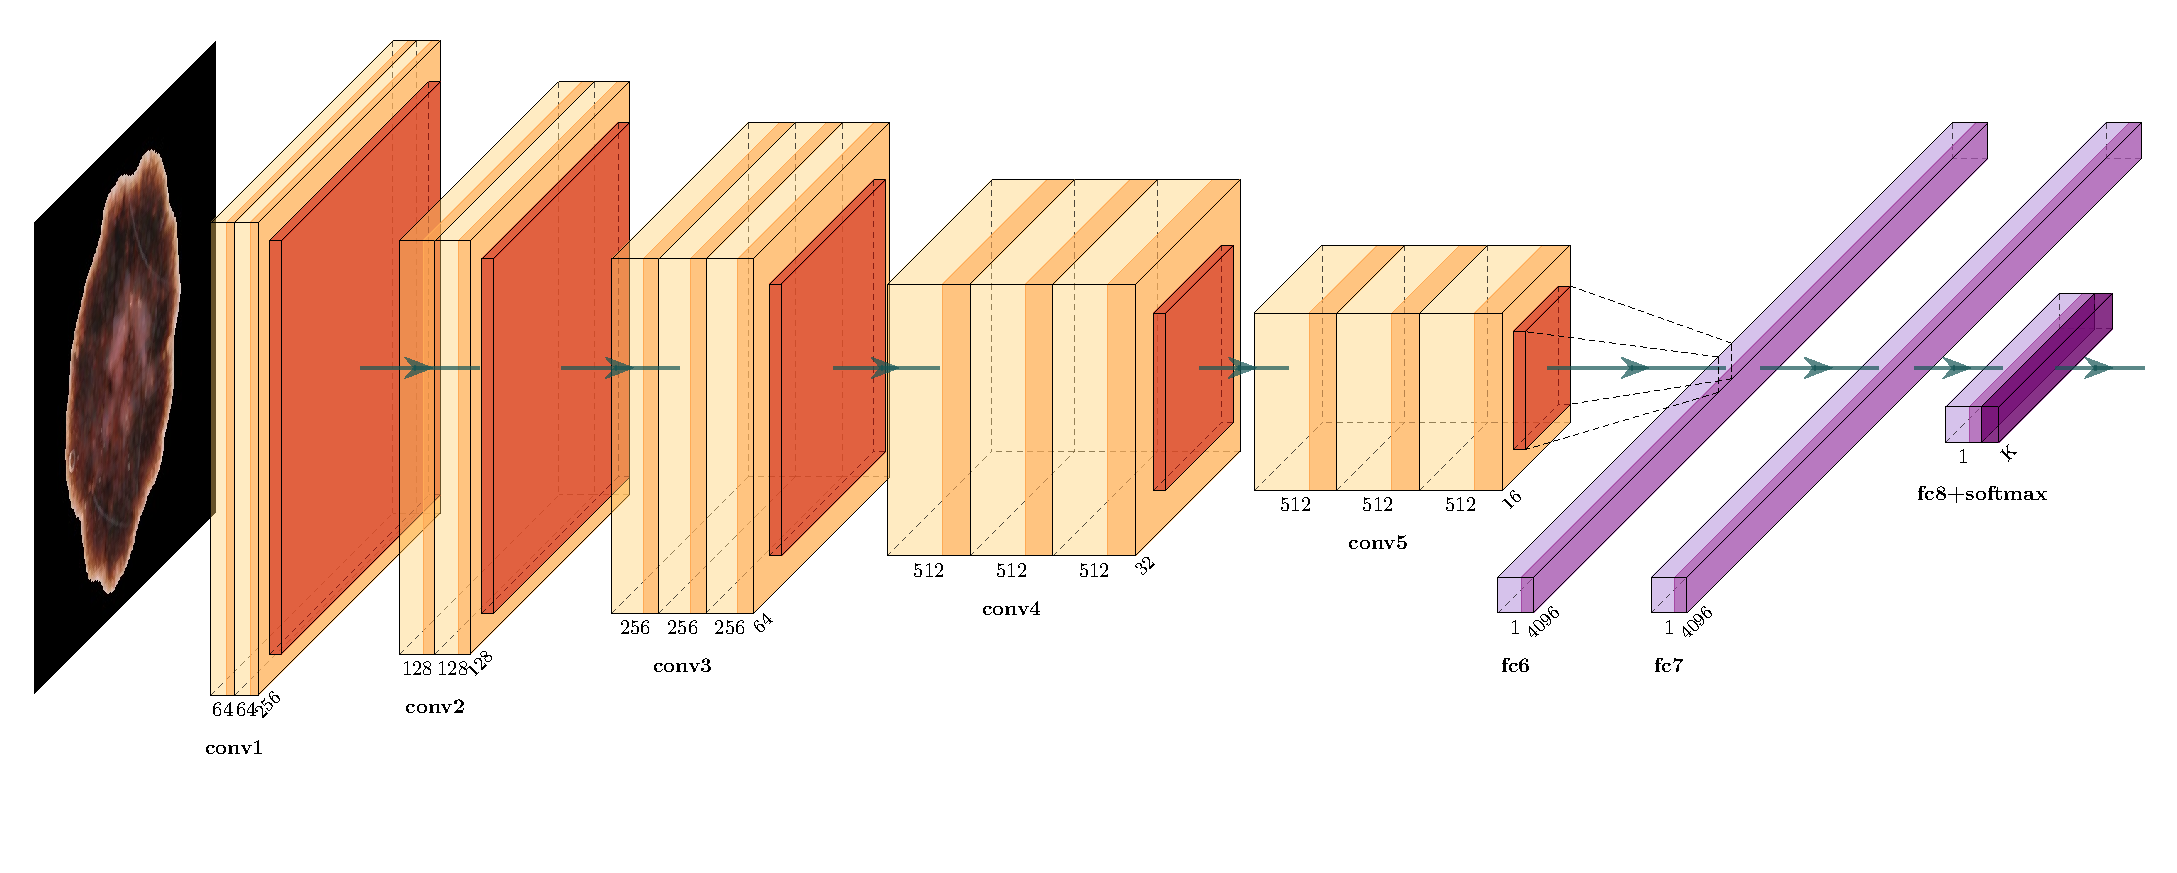
\includegraphics[width=17cm]{Architectures figures/VGG16.pdf}
        \caption[VGG16 architecture]{VGG16 architecture.}
    \end{figure}


     \begin{table}[H]
        \begin{center}
        \begin{tabular}{lll}
            \hline
            \textbf{ Layer (type)} & \textbf{Output Shape} & \textbf{Parameter} \\
            \hline
            Input image & (None, 256, 256, 3) & 0 \\
            VGG16 (Functional) & (None, 512)   & 14714688 \\
            Top flatten (Flatten) & (None, 512) & 0 \\
            Dense 6 (Dense) & (None, 4096) & 2101248 \\
            Dropout 6 (Dropout) & (None, 4096) & 0 \\
            Dense 7 (Dense) & (None, 64) & 262208\\
            Dropout 7 (Dropout) & (None, 64) & 0\\
            Output layer (Dense)  & (None, 1)  & 65\\
        \hline
        \end{tabular}
        \end{center}
        \caption[Details of VGG16 Model Proposed]{\centering Details of VGG16 model proposed.}
    \end{table}



    \subsubsection{EfficientNet}
    \hspace{0.7cm} The EfficientNet is widely acknowledged as one of the largest and most intricate models in DL, rendering its representation is often challenging. Nonetheless, a simple way to represent it is by dividing it into units and showcasing each unit in a sub-block. Subsequently, these sub-blocks are employed to represent different versions of the EfficientNet \cite{agarwal2020complete}.

    \begin{figure}[H]
        \centering
        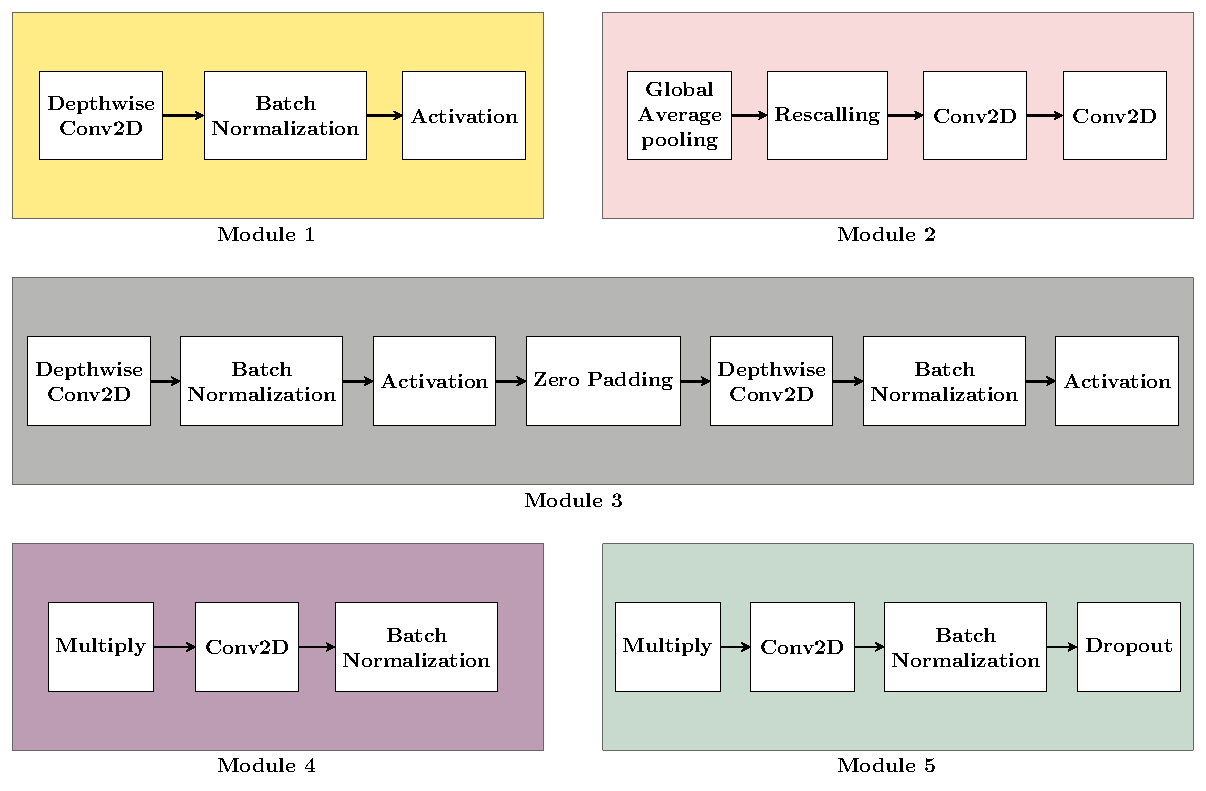
\includegraphics[width=13cm]{Architectures figures/Modules.pdf}
        \caption[EfficientNet Modules architecture]{EfficientNet Modules architecture.}
    \end{figure}

    \begin{figure}[H]
        \centering
        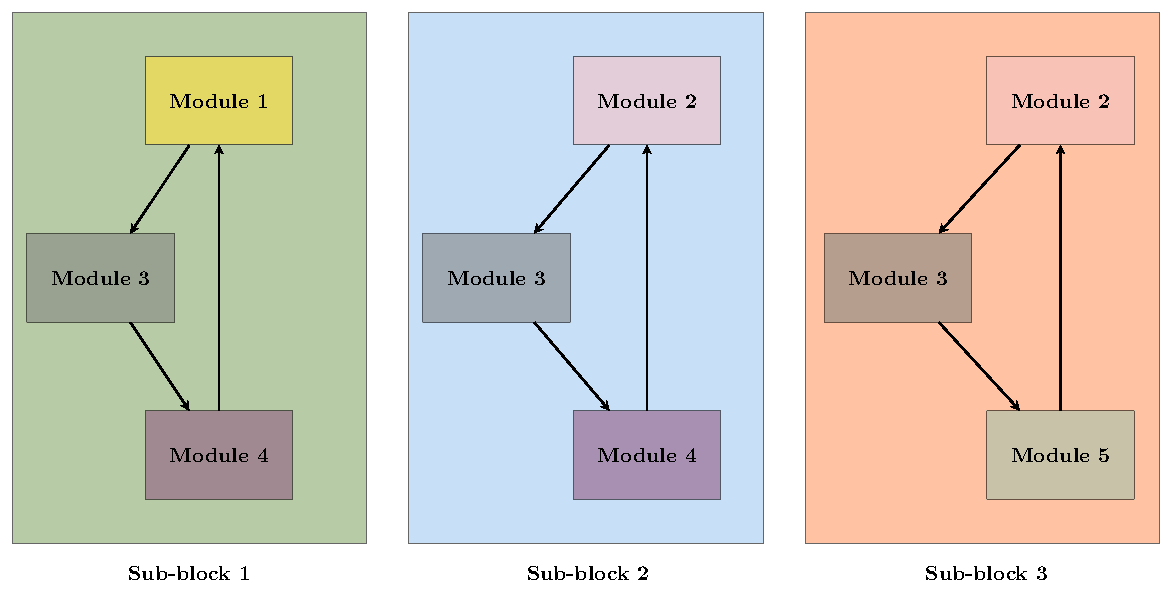
\includegraphics[width=11cm]{Architectures figures/SubBlocks.pdf}
        \caption[EfficientNet SubBlocks architecture]{EfficientNet sub-blocks architecture.}
    \end{figure}
    
    \subsubsubsection{EfficientNetB5}
    
    \begin{figure}[H]
        \centering
        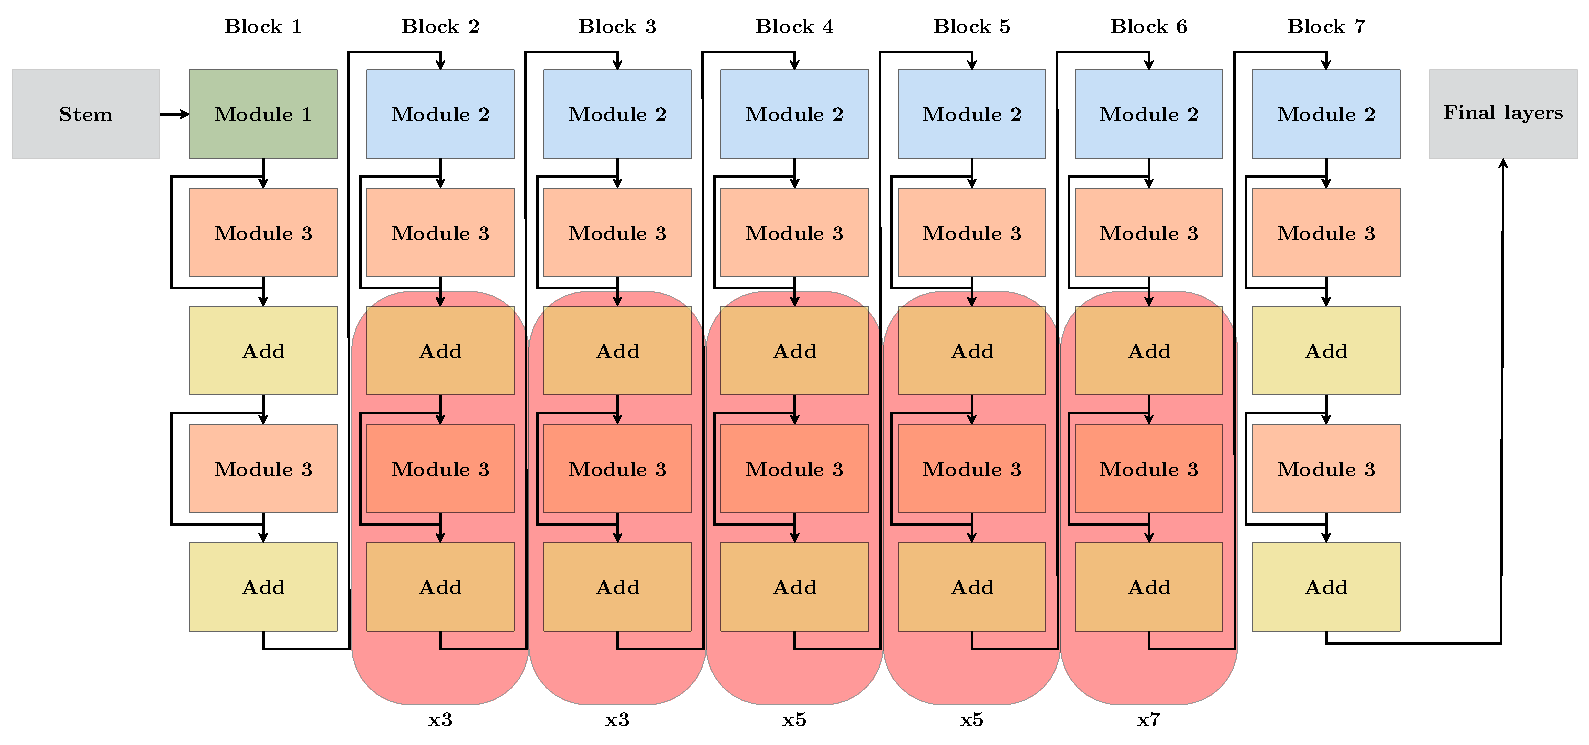
\includegraphics[width=16cm]{Architectures figures/EfficientNetB5.pdf}
        \caption[EfficientNetB5 architecture]{EfficientNet-B5 architecture.}
    \end{figure}

    
    \begin{table}[H]
        \begin{center}
        \begin{tabular}{lll}
            \hline
            \textbf{ Layer (type)} & \textbf{Output Shape} & \textbf{Parameter} \\
            \hline
            Input image & (None, 256, 256, 3) & 0 \\
            EfficientNet-B5 (Functional) & (None, 2048)   & 28513527 \\
            Top flatten (Flatten) & (None, 2048) & 0 \\
            Dense 12 (Dense) & (None, 256) & 524544 \\
            Dropout 12 (Dropout) & (None, 256) & 0 \\
            Dense 13 (Dense)& (None, 32) & 8224\\
            Dropout 13 (Dropout) & (None, 32) & 0\\
            Output layer (Dense)  & (None, 1)  & 33\\
        \hline
        \end{tabular}
        \end{center}
        \caption[Details of EfficientNet-B5 Model Proposed]{\centering Details of EfficientNet-B5 model proposed.}
    \end{table}

    
    \subsubsubsection{EfficientNetB7}

    \begin{figure}[H]
        \centering
        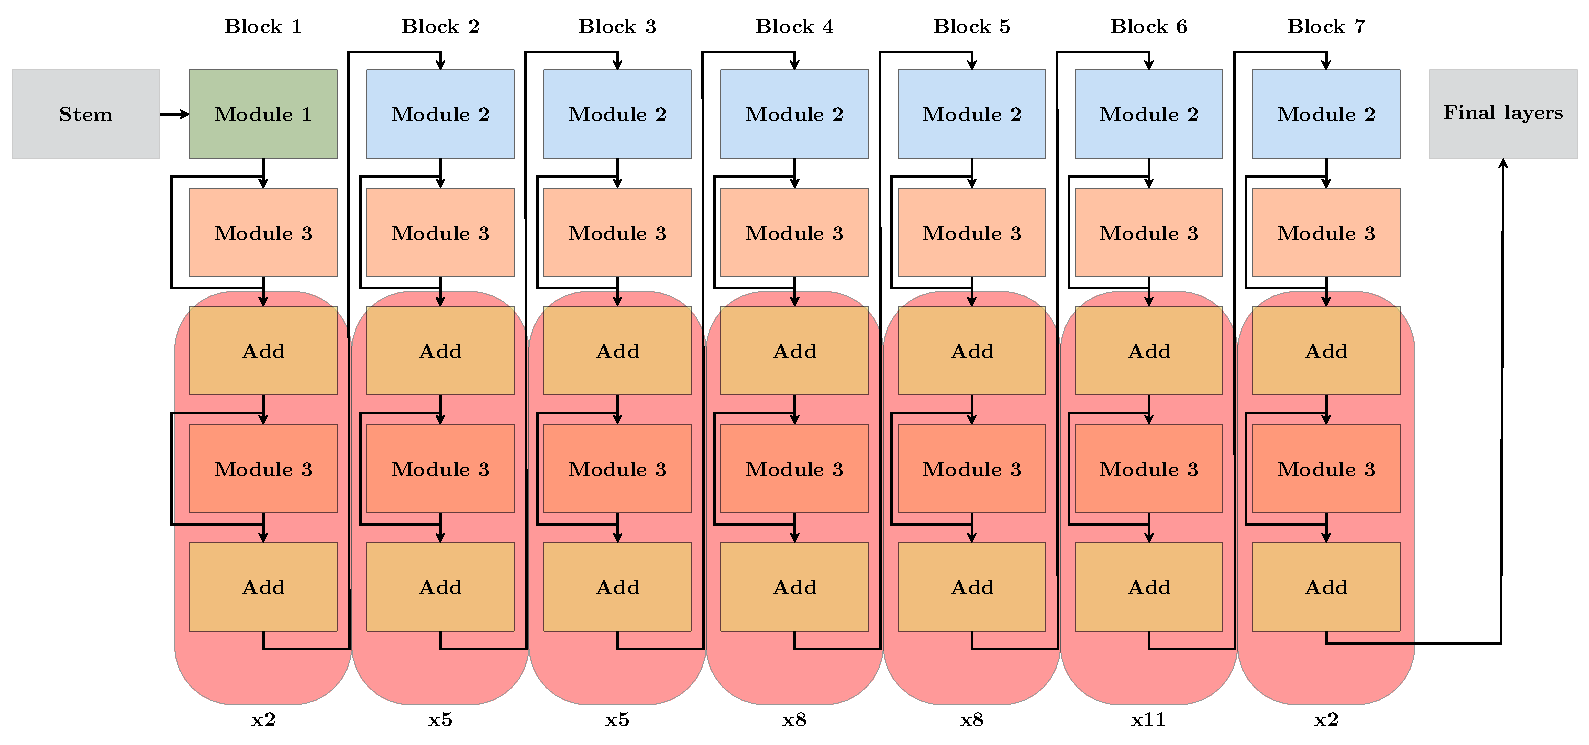
\includegraphics[width=16cm]{Architectures figures/EfficientNetB7.pdf}
        \caption[EfficientNetB7 architecture]{EfficientNet-B7 architecture.}
    \end{figure}
    
    \begin{table}[H]
        \begin{center}
        \begin{tabular}{lll}
            \hline
            \textbf{ Layer (type)} & \textbf{Output Shape} & \textbf{Parameter} \\
            \hline
            Input image & (None, 256, 256, 3) & 0 \\
            EfficientNet-B7 (Functional) & (None, 2560)   & 64097687 \\
            Top flatten (Flatten) & (None, 2560) & 0 \\
            Dense 14 (Dense) & (None, 512) & 1311232 \\
            Dropout 14 (Dropout) & (None, 512) & 0 \\
            Dense 15 (Dense) & (None, 256) & 131328\\
            Dropout 15 (Dropout) & (None, 256) & 0\\
            Output layer (Dense)  & (None, 1)  & 257\\
            \hline
        \end{tabular}
        \end{center}
        \caption[Details of EfficientNetb7 Model Proposed]{\centering Details of EfficientNet-B7 model proposed.}
    \end{table}
    
   
    
    % put Unet Architecture here
    
   %  \textbf{\RomanNumeralCaps { 4. }}  \textbf{Data Augmentation}
   % \\
   % \textbf{\RomanNumeralCaps { 5. }}  \textbf{Model Training}
   % \\

   
    % \-\hspace{0.7cm} In this stage, the classifier model will be designed as a CNN model, in view of the fact that CNN is the DL model that gives the highest rates of the performance measurements among all the DL models as pointed out in Table \ref{tab:references}.\\
    % \-\hspace{0.7cm} For model training, we will use data augmentation to overcome the shortage of images. The model will be trained with malignant lesions images which are resized and denoised.  % in addition to the better performance they reached using GANs. Furthermore, GANs have been recognized as the most dominant generative model in Artificial intelligence \cite{saeed2021skin}, which encouraged us to use it for this task. 
    
    \subsection{SVM Classifier with Feature Extraction}
    %write psuedocode
     \-\hspace{0.7cm} The technique of feature extraction will be employed for the SVM. This method proves to be efficient in decreasing the dimensionality of large datasets, particularly when utilized in conjunction with SVM algorithms, which require a significant amount of computational resources \cite{hira2015review}. By reducing the number of features in the dataset, we can make the training process more efficient and manageable.
    The following features will be extracted from lesion images for skin cancer classification:
    \begin{itemize}
    \item \textbf{Area and Perimeter of the lesion}: These features provide valuable insights into the characteristics of a skin lesion and can be used to distinguish between various types of skin lesions. The area represents the two-dimensional extent of the lesion, while the perimeter indicates the length of the boundary of the lesion. Together, these measurements provide a comprehensive picture of the size and shape of a skin lesion.
    \item \textbf{RGB and HSV}: These features will be used to differentiate between different types of skin lesions based on their color characteristics. RGB values can be used to determine the exact color of a lesion. HSV, on the other hand, can be useful in analyzing the different aspects of the lesion's color. By using both RGB and HSV features, a more comprehensive understanding of the lesion's color can be obtained, which can be useful in differentiating between different types of skin lesions.
    \item \textbf{Mean and Standard Deviation of RGB and HSV}: These features provide information about the distribution of color intensity values in the image and can be used to distinguish between subtle differences in color. By measuring the mean and standard deviation of the RGB and HSV channels, we can quantify the distribution of color information in the image and use that information to differentiate between different types of skin lesions. This information can be especially useful in cases where the differences in color between lesions are subtle, but still important to consider in making a diagnosis.
    \end{itemize}
    
   
    
    \newpage
    \section{Experimental Design}
    \subsection{Dataset}

    \hspace{0.7cm} In order to ensure good generalization in our models, validate their efficiency, and avoid overtraining them, %conventional strategies can be employed. One of those strategies %  
    appropriate data splitting was used. To split the dataset into different sets,  there are several techniques, and we chose the Hold-out technique in this research. Hold-out is a popular technique because of its easiness and efficiency. It divides the dataset T of size n into three subsets,
    training T$_{tr}$, 
    validation T$_{v}$,
    and testing T$_{t}$ of sizes n$_{tr}$, n$_{v}$ and n$_{t}$ consecutively. This technique has the advantage of allowing the proportion of each of these three data subsets to be varied. The model is trained on the training subset T$_{tr}$, while the validation subset T$_{v}$ is used periodically to assess the model's performance during training to prevent overtraining. The training is terminated when the performance on T$_{v}$ is satisfactory or when it ceases to improve. The testing subset T$_{t}$ is then utilized to obtain a reliable estimate of the models' performance \cite{reitermanova2010data}.


    %It is way to split up the dataset into a train validation, and test set. The training set is used to train a model, and the validation set is used to evaluate how well that model performs on unknown data. A common split when using the Hold-out method is using 80\% of the data for training and the remaining 20\% of the data for validation \cite{allibhai2018hold}. This popular split was used.

    \hspace{0.2cm} In this research, the dataset used was collected from the ISIC Archive \cite{ISICdataset}. We split the dataset as follows: 80\% for the training set, 10\% for the validation set, and 10\% for the test set. Dataset's Images Ground-Truth was based on each lesion's medical diagnosis.
    %There were over 8 diagnoses and 3 of them (namely: Melanoma, Basal Cell Carcinoma, and Squamous Cell Carcinoma) are medically identified as malignant types. On this bases, the dataset was divided into two types only: benign and malignant.%
    A total of 20,092 images were used. 11063 images of benign types, and 8732 images of malignant types.
    %This dataset has classified the images as benign and malignant, which matches our goal in Section \ref{section:Goals-and-Objectives}. We used 20,092 images from ISIC dataset, 11063 images of benign lesions, and 8732 images of malignant lesions.
    
   \hspace{0.2cm} Following the pre-processing of the dataset, starting with the segmentation task, 10,015 of the 20,092 images were provided with a mask and were used to train a U-Net model to segment the rest of the images. After segmenting all the images in the dataset, in image generation task, 647 images from the malignant types were used to train a GAN model. The model generated 1299 new images to make the total number of malignant class images 10031. 
   
   
   %To test our models' performance, the $PH^2$ dataset was used. $PH^2$ has 200 dermoscopic images of melanocytic lesions, 160 benign lesion images, and 40 malignant ones. 
   
   %Eventually, in the classification task, all images were use idiagnosesign class after segmentation (which are 11063 as mentioned above), and the 10031 images in the malignant class with the generated images by the GAN model.


    \subsection{Experiments}
    \hspace{0.7cm} In this step, we will experiment with the models mentioned in the methodology: The CNN model, CNN with data augmentation using GAN model, and SVM model. Four different tests will be conducted. \\
        \textbf{\RomanNumeralCaps { 1. } CNN Classifiers Test} \\
        \-\hspace{0.7cm} We will conduct the first test by taking a subset of images and preprocess them by resizing them, and then denoise them using the DullRazor technique. A U-Net network will be used to output a mask for each image, and the mask will be applied to the images to remove the background, and finally, the output dataset will be used to train the pre-trained CNN classifiers. %we will take e the denoised images with their segmented version (masks), and train the model to automatically output an image mask and segment it using U-Net technique. Finally, we will train the classifier with the images we obtained from the segmenter to classify it by their label (Benign/Malignant).
        \\
        \textbf{\RomanNumeralCaps { 2. } CNN Classifiers with Data Augmentation using GAN}\\
        \-\hspace{0.7cm} For the second test, we shall use the same aforementioned process provided that we will add an extra step after the pre-processing. We will take the pre-processed malignant lesions images to generate more data using GAN, and then we will train, test and evaluate our pre-trained CNN models again.
        \\ 
        \textbf{\RomanNumeralCaps { 3. } SVM Classifier}\\ 
        \-\hspace{0.7cm}  In this test, we will implement an SVM model using our pre-processed and segmented images to compare the results with our CNN models before the data augmentation step.
        \\
        \textbf{\RomanNumeralCaps { 4. } SVM Classifier with Data Augmentation using GAN}\\
        \-\hspace{0.7cm} Finally, the same previously mentioned SVM model will be used, and the pre-processed malignant lesions images will be trained to generate more data using GAN, and the results in this test will be compared with the results in the second test.

       
    \newpage
    \section{Implementation Details}
    \subsection{Implementation Environment}
    \-\hspace{0.7cm}In order to implement our experiments, we have chosen Python as it is the most suitable programming language for ML and DL experiments. It provides a variety of libraries to support the implementation process. As implementing these experiments consumes a lot of hardware resources, Google Colaboratory was our choice to run them. The reason for this is that it provides cloud-based resources like GPUs. We used several libraries, including TensorFlow's Keras, OpenCV, Scikit-Learn, and SciPy.

    \textbf{Keras} is a Python-based DL API that runs on top of TensorFlow and provides a high-level interface for developing DL neural networks \cite{manaswi2018understanding}.

    \textbf{OpenCV} is an open-source Python library used for image processing and computer vision. Many algorithms are available that can be used to identify objects, detect and recognize faces, and more \cite{bradski2008learning}.

    \textbf{Scikit-Learn} is an open-source Python library for ML and statistical modeling. Among its features are algorithms for classification, regression, clustering, and dimension reduction, as well as unsupervised and supervised learning techniques \cite{pedregosa2011scikit}.

    \textbf{SciPy} is a library that takes on standard problems, and mathematical computations, using arrays and manipulations \cite{bressert2012scipy}.

    \subsection{Preprocessing}

    \-\hspace{0.7cm}In order to provide a clear understanding of our models workings, we will provide a pseudocode of algorithms used through out this experiment.
    Our experiment with the DullRazor algorithm have produced intriguing results, which demonstrate its effectiveness in detecting and removing hair from images. \\
    
    
    \begin{algorithm}[H]
        \DontPrintSemicolon
        \SetKwInOut{Input}{Input}
        \SetKwInOut{Output}{Output}
    
        \Input{Image Array}
        \Output{Image Array After Applying DullRazor Algorithm} 
    
        $grayimage = \mathbf{RGB2GRAY}(image)$\;
        $blackhat = \mathbf{MorphologyEx}(grayimage, MORPH\_BLACKHAT, filter_{9\times9})$\;
        $blurredimage = \mathbf{GaussianBlur}(blackhat, filter_{3\times3})$\;
        $mask = \mathbf{BinaryThreshold}(blurredimage, threshold=15, maxval=255)$\;
        $output = \mathbf{Inpaint}(image, mask, inpaintRadius = 6, INPAINT\_TELEA)$\; 
        
        \caption{DullRazor}
    \end{algorithm} 

    The algorithm was implemented using OpenCV library. Figure \ref{fig:DullRazorOutput} shows a sample of images processed by the DullRazor algorithm. 

    \begin{figure}[htp]
        \centering
        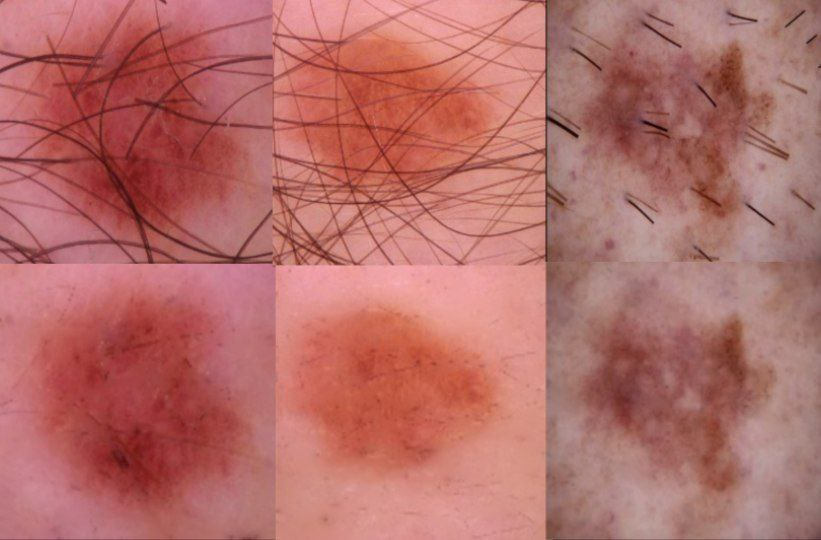
\includegraphics[width=9cm]{Figures/DullRazorOutput.jpg}
        \caption[Sample output of the DullRazor]{Sample output of the DullRazor.}
        \label{fig:DullRazorOutput}
    \end{figure}
    
    \subsection{Segmentation}
    \hspace{0.7cm} The below algorithm shows a pseudocode for U-Net algorithm witch used in segmentation task.\\

    
    \begin{algorithm}[H]
        \DontPrintSemicolon
        \SetKwInOut{Input}{Input}
        \SetKwInOut{Output}{Output}
        
        \Input{DIR "Dataset directory"}
        \Output{masks for images with no available mask} 
        
            (trainingData, trainingMasks), (validationData, validationMasks) $\gets$ loadDataset(DIR=DIR) \;
        $model$ $\gets$ getUNet() \;
        callbacks $\gets$ CSVLogger and ModelCheckpoint callbacks \;
        
            model.fit(trainingData, trainingMasks, batchSize=32, epochs=30, validationData=(validationData, validationMasks), callbacks=callbacks)\;

        images $\gets$ loadDatasetWithNoMask() \;
        masks $\gets$ empty set \;
        \For{image $\in$ images}{
            prediction $\gets$ $model$.predict(image) \;

            mask $\gets$ applyOtsuThreshold(prediction) \;
            append mask to masks \;
        }

        \caption{U-Net Model Training Function}
        
        \label{alg:UnetTraining}
    \end{algorithm}

    \begin{figure}[htp]
        \centering
        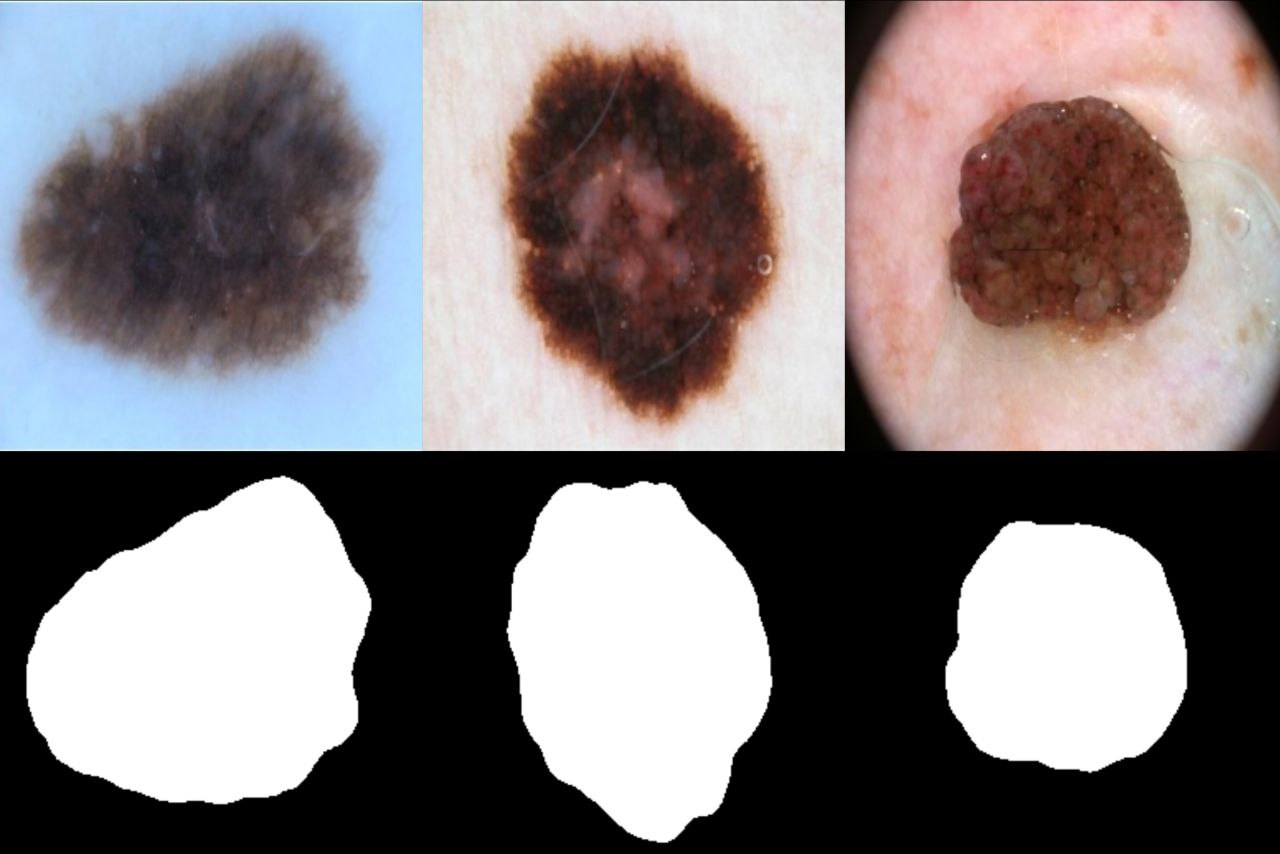
\includegraphics[width=9cm]{Figures/UnetOutput.jpg}
        \caption[Sample Output of U-Net Image segmentation]{Sample output of U-Net image segmentation.}
        \label{fig:UnetOutput}
    \end{figure}

    \newpage
    \subsection{Augmentation}
    \hspace{0.7cm} The pseudocode below represents a GAN algorithm witch used in data augmentation task.\\

    \begin{algorithm}[H]
       \DontPrintSemicolon

        \For{number of training iterations}{
            \For{k steps}{
                Sample minibatch of $m$ noise samples ${z^{(1)},...,z^{(m)}}$ from noise prior $p_g(Z)$. \;
                Sample minibatch of m examples ${x^{(1)},...,x^{(m)}}$  from data generating distribution $p_{data}(x)$. \;
                Update the discriminator by ascending its stochastic gradient: \;
                $\nabla_{\theta_{d}}\frac{1}{m}\sum_{i= 1}^{m}[\log D(x^{(i)}) + \log (1- D(G(z^{(i)})))]$\;
            }
            Sample minibatch of $m$ noise samples ${z^{(1)},...,z^{(m)}}$ from noise prior $p_g(Z)$. \;
            Update the generator by descending its stochastic gradient: \;
            $\nabla_{\theta_{g}}\frac{1}{m}\sum_{i= 1}^{m} \log (1- D(G(z^{(i)})))$\;
        }

        \caption{Minibatch Stochastic Gradient Descent training of Generative Adversarial Nets \cite{Goodfellow2014-cu}} %The number of steps to apply to the discriminator, $k$, is a hyperparameter.}
    \end{algorithm}

    \newpage
 
    \begin{figure}[htp]
        \centering
        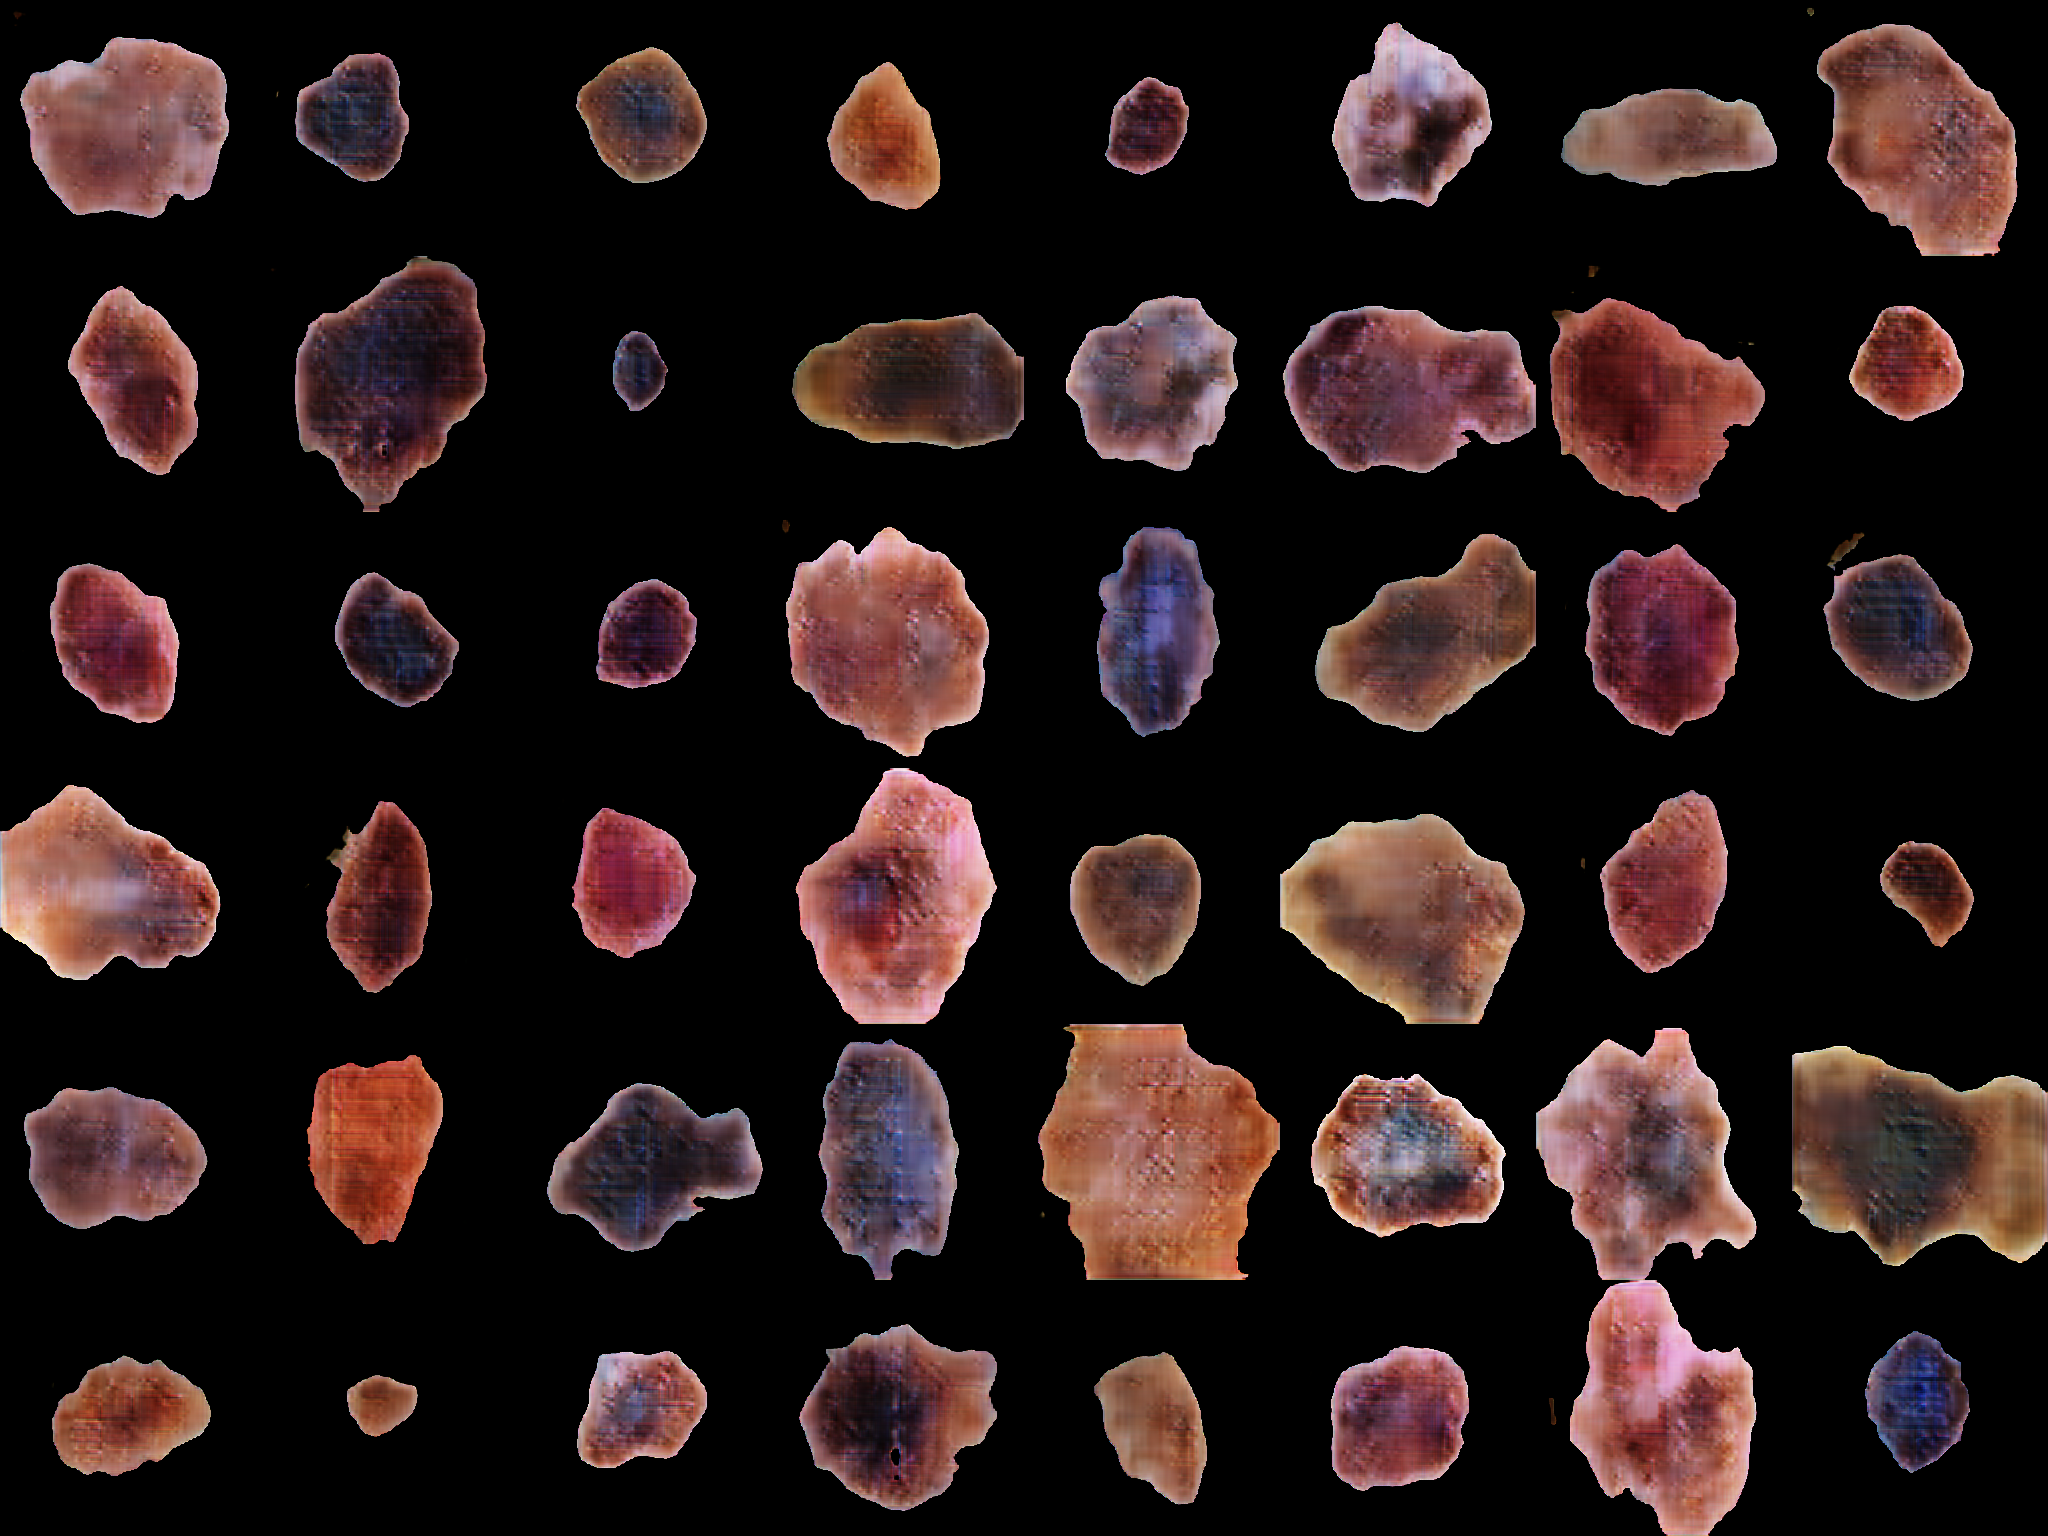
\includegraphics[width=9cm]{Figures/GANOutput.png}
        \caption[Sample Output of GAN model]{Sample output of the GAN model.}
        \label{fig:GANOutput}
    \end{figure} 
    
   \subsection{Classification}
    
    \subsubsection{SVM}


    \hspace{0.7cm} In the image classification task using SVM, the model is available in Scikit-learn, we trained the model as shown in the algorithm below. \\

    \begin{algorithm}[H]
    \DontPrintSemicolon
    \SetKwInOut{Input}{Input}
    \SetKwInOut{Output}{Output}
    
    \Input{Images' extracted features}
    \Output{Trained SVM model}
    
    
        dataset $\gets$ Images Features \;
        train, test $\gets$ SplitData(dataset) \;
        dataset $\gets$ StandardScalar(dataset)\;
        model = SVM()\;
        %model $\gets$ train SVM model with GridSearchCV\;
        model.fit(train, trainLabels)\;
        %parameters $\gets$ model.BestParameters \;
        model.evaluate(test, testLabels)  \;
        Save the model and its accuracy report \;
    
    \caption{SVM}
    \label{alg:svmclassifierTraining}
    \end{algorithm}


    \subsubsection{CNN}

    \hspace{0.7cm} For an image classification task using CNN, the four pre-trained models are available in tensorflow.keras.applications module, models were trained using a training loop as shown in the pseudocode algorithm \ref{alg:cnnclassifierTraining}.

    
    % For an image classification task, the following four DL models have been selected:

    % \begin{itemize}
    % \item \textbf{EfficientNetB7}: A highly efficient and scalable Convolutional Neural Network (CNN) model that was developed by Google. It is designed to achieve high accuracy with minimal computational resources, making it ideal for deployment on devices with limited resources. EfficientNetB7 is an updated version of the original EfficientNet model and has achieved state-of-the-art performance on a variety of image classification benchmarks.
    % \item \textbf{EfficientNetB5}: Another version of the EfficientNet model that offers a trade-off between accuracy and computational efficiency. It has a slightly smaller architecture compared to EfficientNetB7, but still delivers good performance for image classification tasks.
    % \item \textbf{ResNet50V2}: A Residual Network (ResNet) model that was developed by Microsoft Research. ResNets are known for their ability to train very deep networks effectively and ResNet50V2 is a popular choice for image classification tasks. It has 50 convolutional layers and is pre-trained on the ImageNet dataset, making it a good starting point for a variety of image classification tasks.
    % \item \textbf{VGG16}: A classic Convolutional Neural Network (CNN) model that was developed by the Visual Geometry Group at the University of Oxford. VGG16 is known for its simple architecture and good performance on image classification tasks. It is a good choice for a baseline model, or for tasks where computational efficiency is not a primary concern.
    % \end{itemize}

    % These four models provide a diverse set of architectures, computational requirements, and performance characteristics, making them suitable for our task, and are available in tensorflow.keras.applications module, models were train using a training loop as shown in pseudocode algorithm \ref{alg:cnnclassifierTraining}.

    \begin{algorithm}[H]
    \DontPrintSemicolon
    \SetKwInOut{Input}{Input}
    \SetKwInOut{Output}{Output}
    
    \Input{preTrainedModels a dictionary containing transfer learning models as keys and model parameters as value}
    \Output{Models' testing results}
    
    results $\gets$ empty DataFrame \;
      \For{preTrainedModel $\in$ preTrainedModels dictionary}{
        \For{dataset $\in$ datasets}{
            % get model parameters from preTrainedModels \;
            parameters $\gets$ preTrainedModels[preTrainedModel] \;
            epochs $\gets$ parameters.epochs \;
            train, validate, test $\gets$ getDataset(DIR=dataset, BATCHSIZE=parameters.batchSize) \;
            $model \gets$ getModel(preTrainedModel, learningRate=parameters.learningRate, pooling=parameters.pooling, dropout=parameters.dropout, denseSize=parameters.denseSize)\;
            callbacks $\gets$ modelCallbacks() \;
            $model$.train(train, validate, callbacks=callbacks)  \;
            result $\gets model$.evaluate(test, batchSize=parameters.batchSize) \;
            get evaluation result and store it as a dictionary \;
            calculate F1 Score using recall and precision \;
            add Model and dataset names, and F1 Score to the result dictionary \;
            create a DataFrame from the result dictionary \;
            append the DataFrame to the results DataFrame \;
        }
    }
    \caption{Models Training Loop}
    
    \label{alg:cnnclassifierTraining}
    \end{algorithm}




    \subsection{Evaluation methods}
  
    \-\hspace{0.7cm} In order to make results clear and accurate as possible, in the classification task, all the models had been evaluated using the four performance measurements mentioned in the Background, which are: Accuracy, Precision, Recall, and F1 Score.

    
    \subsection{Implementation Issues}
    \-\hspace{0.7cm} The implementation of large-scale DL models often involves various hardware and resource management challenges. These challenges can be particularly pronounced when using limited resources such as those available through Google Colaboratory. During the course of our experiment, we encountered several significant issues related to GPU and storage space management. These issues required careful planning and resource allocation to overcome. Despite these challenges, we were able to successfully implement the DL model and obtain meaningful results. However, it is important to note that proper hardware and resource management is crucial for the successful deployment of DL models, especially when working with limited resources.

    \newpage
    \section{Results and Discussion}
    \-\hspace{0.7cm} In this chapter, we present our models' test result and provide a detailed analysis of the performance metrics of our trained models.
    
    \subsection{Parameters Tuning} 
    %Deep learning hyperparameter tuning is the process of adjusting the hyperparameters of a deep learning model to improve its performance. Hyperparameters are model parameters that are set before training and are not learned from the data during the training process. They include things like the learning rate, number of hidden layers, and batch size. The optimal values of these hyperparameters can have a significant impact on the performance of a deep learning model, and finding the right combination can be challenging and time-consuming.

    %Keras-Tuner is a hyperparameter tuning library for Keras, a popular deep learning framework. It provides a convenient and efficient way to search for the optimal hyperparameters for a Keras model. It offers a variety of tuners, including random search, grid search, and Bayesian optimization, and it also supports custom tuners. Keras-Tuner makes it easy to use hyperparameter tuning in your deep learning projects, and it can help you find the best hyperparameters for your models in a fraction of the time it would take to do it manually. Additionally, it integrates well with other libraries, making it easy to use in your existing workflows.


    \-\hspace{0.7cm} Hyperparameter tuning is one of the fundamental ways to enhance the performance of ML models. During the learning process of a model, hyperparameters are passed in order to make corrections or adjustments. Diverse data patterns may necessitate distinct constraints, weights, or learning rates for the same ML model. These kinds of measurements are referred to as hyperparameters \cite{pon2021hyperparameter}.

    
     \subsubsection {SVM Tuning}
     \-\hspace{0.7cm} We tuned the hyperparameters of our SVM model by using Grid Search. Grid Search, also known as the Estimator, is a tuning technique aiming to calculate hyperparameters' optimal values. It is an exhaustive search that is performed on specific parameter values of a specific model \cite{malik2020grid}. \\

     The ranges of values to tune the hyperparameter in SVM are as follows:
    \begin{itemize}
     \item C: [0.001, 0.01, 0.1, 1, 10, 100, 1000]
     \item kernel: [linear, poly, rbf, sigmoid]
      \item gamma: [0.0001, 0.001, 0.01, 0.1, 1, 10, scale, auto].
     \end{itemize}

     \subsubsection {SVM Tuning Results}

    \-\hspace{0.7cm} After performing the grid search, the optimal hyperparameters for our SVM model were found to be C = 1000, gamma = auto, and kernel = rbf. This indicates that a high value of C, the radial basis function (RBF) kernel, and an automatic setting for gamma were the best choices for our problem.



    \subsubsection {CNN Tuning}
     \-\hspace{0.7cm} To tune the hyperparameters of our DL models, we used KerasTuner, which is a scalable, easy-to-use hyperparameter optimization framework that alleviates the difficulties associated with hyperparameter search. KerasTuner comes with Bayesian Optimization, Hyperband, and Random Search algorithms, and is designed to be extensible so that researchers can experiment with new search algorithms \cite{chollet2015keras}.

     The hyperparameters we tuned are:
     \begin{enumerate}
     \item Dropout
     \item Dense layers sizes
     \item Learning Rate 
     \item Pooling type
     \end{enumerate}

     Each hyperparameter has a range of values to make the tuner decide which value is more suitable, the ranges of values are as follows:
     \begin{itemize}
     \item Dropout 1: Range [0, 0.8]
     \item Dsense layer 1: [4096, 512, 256]
     \item Dropout 2: Range [0, 0.6]
     \item Dsense layer 2: [128, 64, 32]
     \item Learning Rate: Range [1e-4, 1e-7]
     \item Pooling type: [Average, Max]
   \end{itemize}

    \subsubsection {CNN Tuning Results}
    \-\hspace{0.7cm} Using the above mentioned processing techniques and model parameter tuning libraries. We present the results of the models on the test set using two datasets, where we added augmentation data in one, demonstrating the effectiveness of the proposed approach.


   \begin{table}[H]
    \begin{center}
    \makebox[0cm]{
        \begin{tabular}{lcccl}
        \toprule
        \textbf{Model} & \textbf{Dropouts} & \textbf{Dense layers} & \textbf{Learning Rate} & \textbf{Pooling type} \\
        \midrule
        EfficientNetB5 & [.4, .2] & [256, 32] & 1e-05 & Average pooling \\
        EfficientNetB7 & [.8, .6] & [512, 256] & 7e-5 & Max pooling \\  
        ResNet50V2 & [.3, .1] & [4096, 32] & 9e-06 & Average pooling \\
        VGG16 & [.3, .0] & [4096, 64] & 5e-06 & Max pooling\\
        \bottomrule
        \end{tabular}
        \label{table:models}
    }
    \end{center}
    \caption{Models Configurations.}
    \end{table}

     

    \subsection{Results}
    \-\hspace{0.7cm} As the primary objective of our research was to investigate the effectiveness of DL algorithms in accurately classifying skin lesions as either malignant or benign. In this chapter, we provide a detailed analysis of the performance metrics of our trained models and compare them with existing methods.

    \begin{table}[H]
    \begin{center}
    \makebox[0cm]{
    \begin{tabular}{llrrrr}
    \toprule
    \textbf{Model} & \textbf{Dataset} & \textbf{Accuracy} & \textbf{Recall} & \textbf{Precision} & \textbf{F1 Score} \\
    \midrule
        EfficientNet-B7 & Segmented & 0.856219 & 0.882151 & 0.805643 &  0.842163 \\
        \textbf{EfficientNet-B7} & \textbf{Segmented and augmented} &  \textbf{0.869159} & \textbf{0.862550} & \textbf{0.859127} &  \textbf{0.860835} \\
        EfficientNet-B5 & Segmented &  0.843781 & 0.737986 & 0.883562 &  0.804239 \\
        \textbf{EfficientNet-B5} & \textbf{Segmented and augmented} &  \textbf{0.855140} & \textbf{0.797809} & \textbf{0.882159} &  \textbf{0.837866} \\
        ResNet50V2 & Segmented &  0.831343 & 0.779176 &   0.823458 &  0.800705 \\
        \textbf{ResNet50V2} & \textbf{Segmented and augmented} &  \textbf{0.852804} & \textbf{0.833665} & \textbf{0.849746} &  \textbf{0.841629} \\
        VGG16 & Segmented &  0.840796 & 0.779176 &   0.842822 &  0.809750 \\
        \textbf{VGG16} & \textbf{Segmented and augmented} &  \textbf{0.841121} & \textbf{0.795817} & \textbf{0.855460} & \textbf{0.824561} \\
    \bottomrule
    \end{tabular}
    }
    \end{center}
    \caption{CNN Models testing results.}
    \label{tab:CNN results}
    \end{table}

    \begin{figure}[H]
        \centering
        \begin{minipage}[b]{0.45\textwidth}
            \centering
            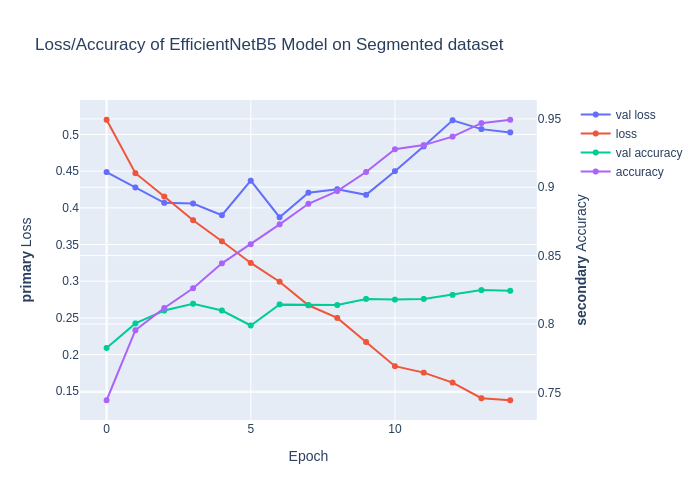
\includegraphics[width=\textwidth]{charts/EfficientNetB5_classification.png}
            \caption{\small {EfficientNet-B5}}
        \end{minipage}
        \hfill
        \begin{minipage}[b]{0.45\textwidth}
            \centering
            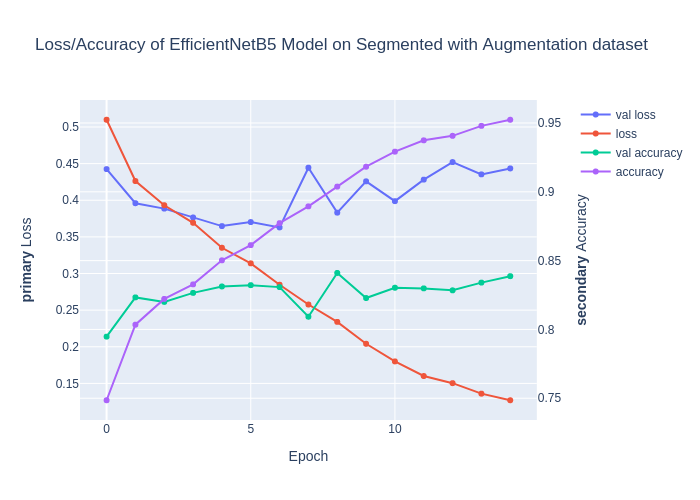
\includegraphics[width=\textwidth]{charts/EfficientNetB5_classificationWithGAN.png}
            \caption{\small {EfficientNet-B5 with GAN}}
        \end{minipage}
    \end{figure}

    \begin{figure}[H]
        \centering
        \begin{minipage}[b]{0.45\textwidth}
            \centering
            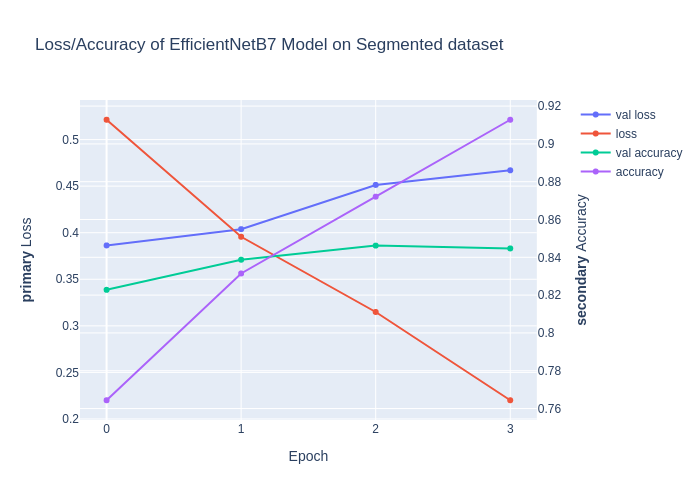
\includegraphics[width=\textwidth]{charts/EfficientNetB7_classification.png}
            \caption{\small{EfficientNet-B7}}
        \end{minipage}
        \hfill
        \begin{minipage}[b]{0.45\textwidth}
            \centering
            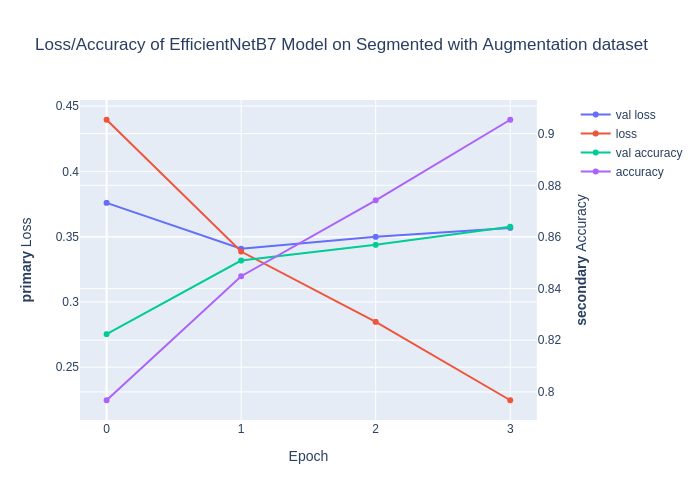
\includegraphics[width=\textwidth]{charts/EfficientNetB7_classificationWithGAN.png}
            \caption{ \small{ EfficientNet-B7 with GAN}}
        \end{minipage}
    \end{figure}

    \begin{figure}[H]
        \centering
        \begin{minipage}[b]{0.45\textwidth}
            \centering
            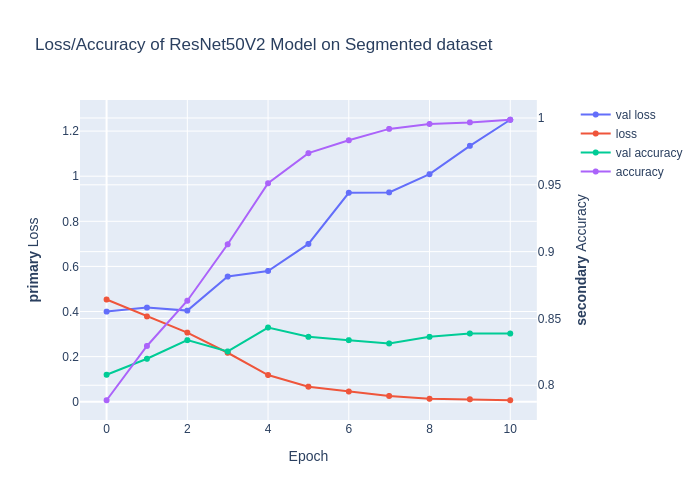
\includegraphics[width=\textwidth]{charts/ResNet50V2_classification.png}
            \caption{\small{ResNet50V2}}
        \end{minipage}
        \hfill
        \begin{minipage}[b]{0.45\textwidth}
            \centering
            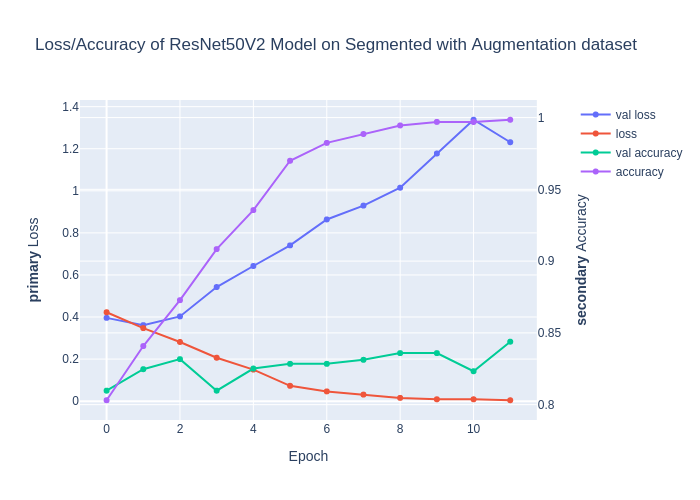
\includegraphics[width=\textwidth]{charts/ResNet50V2_classificationWithGAN.png}
            \caption{\small{ResNet50V2 with GAN}}
        \end{minipage}
    \end{figure}

    \begin{figure}[H]
        \centering
        \begin{minipage}[b]{0.45\textwidth}
            \centering
            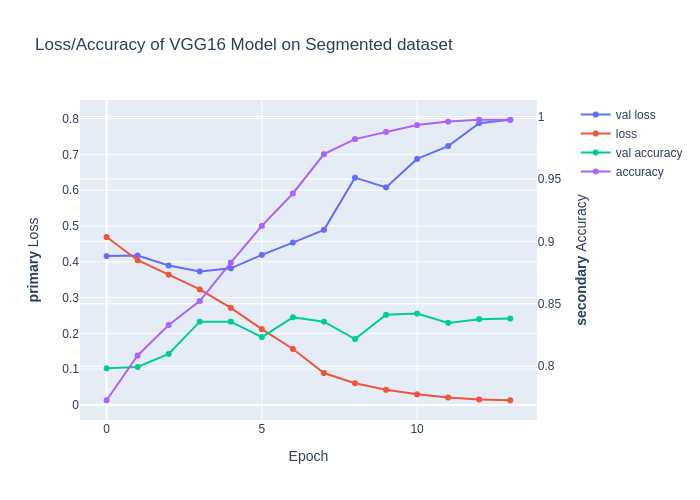
\includegraphics[width=\textwidth]{charts/VGG16_classification.png}
            \caption{\small{VGG16}}
        \end{minipage}
        \hfill
        \begin{minipage}[b]{0.45\textwidth}
            \centering
            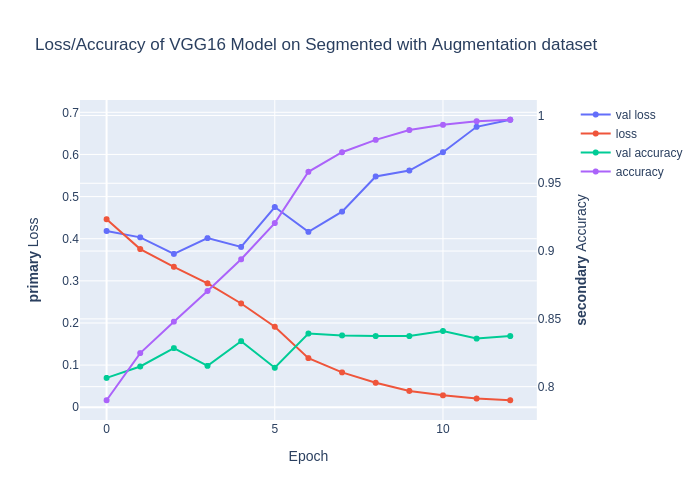
\includegraphics[width=\textwidth]{charts/VGG16_classificationWithGAN.png}
            \caption{ \small {VGG16 with GAN}}
        \end{minipage}
    \end{figure}

    \begin{figure}[htbp]
        \centering
        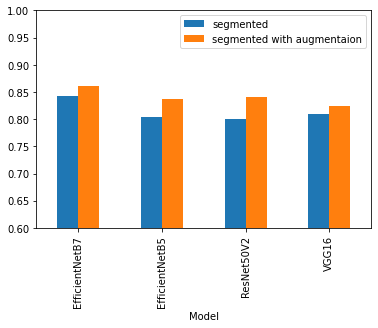
\includegraphics[width=8cm]{charts/ComparingF1Scores.png}
        \caption[comparing models' F1 Scores]{Comparing Models' F1 Scores.}
        \label{tab:SVM results}
    \end{figure} 


    \begin{table}[H]
    \begin{center}
    \makebox[0cm]{
    \begin{tabular}{llrrrr}
    \toprule
    \textbf{Dataset} & \textbf{Accuracy} & \textbf{Recall} & \textbf{Precision} & \textbf{F1 Score} \\
    \midrule
       Segmented & 0.748693 & 0.657175 & 0.738796 &  0.695600 \\
    \textbf{Segmented and augmented} &  \textbf{0.757419} & \textbf{0.716915} & \textbf{0.754450} &  \textbf{0.735204} \\

    \bottomrule
    \end{tabular}
    }
    \end{center}
    \caption{SVM testing results.}
    \end{table}
    
    % \begin{figure}[H]
    %    \centering
    %       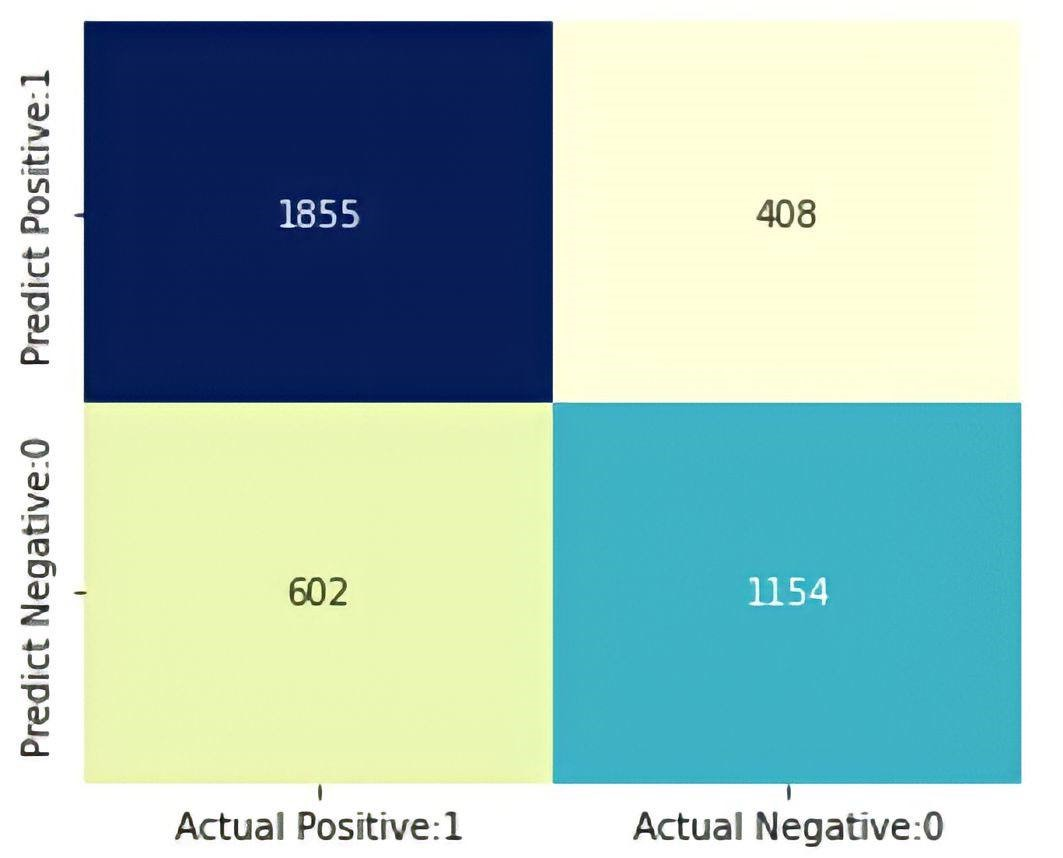
\includegraphics[width=9cm]{charts/SVM.jpg}
    %      \caption{SVM Confusion matrix}
    %\end{figure} 

    %   \begin{figure}[H]
    %      \centering
    %        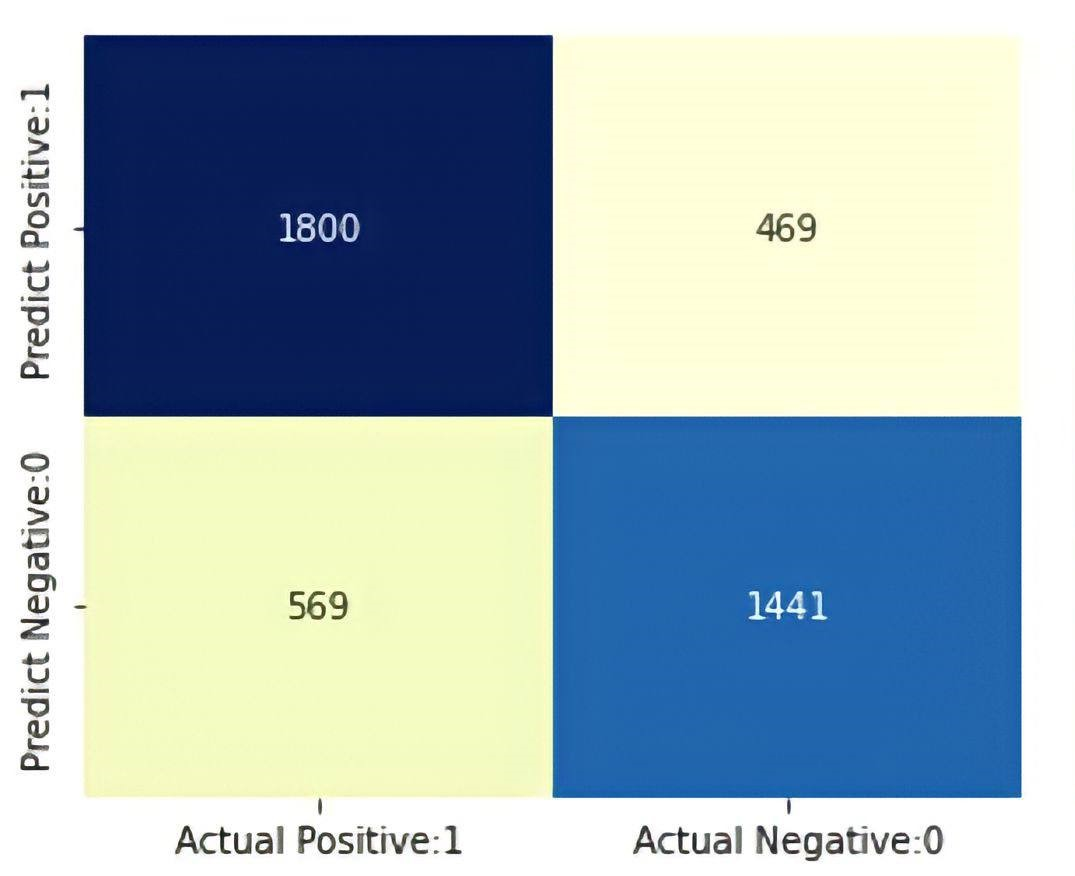
\includegraphics[width=9cm]{charts/SVMwithGAN.jpg}
    %      \caption{SVM with augmentation Confusion matrix}
    %\end{figure} 

    %\subsubsection{Segmented Dataset}
    %\begin{tabular}{lrrrr}
    %\toprule
    %{}  & Accuracy &  precision &    recall &  F1 Score \\
    %\midrule
    %False        & 0.748693 &   0.754986 &  0.819708 &  0.786017 \\
    %True         &   {}     &   0.738796 &  0.657175 &  0.695600 \\
    %macro avg    &   {}     &   0.746891 &  0.738442 &  0.740808 \\
    %weighted avg &   {}     &  0.747912 &  0.748694 &  0.746511 \\
    %\bottomrule
    %\end{tabular}
    %\subsubsection{Segmented and augmented}
    %\begin{tabular}{lrrrr}
    %\toprule
    %{} & Accuracy &  precision &    recall &  F1 Score  \\
    %\midrule
     %False  & 0.757419 &  0.759814 &  0.793301 &  0.7776197 \\
     %True         &   {} & 0.754450 &  0.716915 &  0.735204  \\
     %macro avg    &  {} & 0.757132 &  0.755108 &  0.755700  \\
     %weighted avg &  {} & 0.757295 &  0.757420 &  0.756941 \\
    %\bottomrule
    %\end{tabular}


    %    \begin{center}
    %    \makebox[0cm]{
    %    \begin{tabular}{llrrrr}
    %    \toprule
    %    \textbf{Model} & \textbf{Dataset} & \textbf{Accuracy} & \textbf{Recall} & \textbf{Precision} & \textbf{F1 Score} \\
    %    \midrule

    % SVM & Segmented and augmented &  0.757419 & 0.716915 & 0.754450 &  0.735204 \\
    
    %        \textbf{EfficientNetB7} & \textbf{Segmented and augmented} &  \textbf{0.869159} & \textbf{0.862550} & \textbf{0.859127} &  \textbf{0.860835} \\     
    %    \bottomrule
    %    \end{tabular}
    %    }
    %    \end{center}


    

    \subsection{Performance Analysis}

    The following table (Table \ref{tab:Time Complexity}) shows the time complexity for SVM model and for each of the CNN models using datasets and without augmented data. Additionally, we used Google's colab that have over 500 GPUs to speed up the run.\\
    
    \begin{table}[H]
    \begin{center}
    \makebox[0cm]{
    \begin{tabular}{llc}
    \toprule
    \textbf{Model} & \textbf{Dataset} & \textbf{Training Time}  \\
    \midrule
        EfficientNetB7 & Segmented & 1253 s \\
        
        \textbf{EfficientNetB7} & \textbf{Segmented and augmented} &  \textbf{1325 s}  \\
        
        EfficientNetB5 & Segmented & 6003 s   \\
        
        \textbf{EfficientNetB5} & \textbf{Segmented and augmented} &  \textbf{6368 s} \\
        
        ResNet50V2 & Segmented &  787 s   \\
        
        \textbf{ResNet50V2} & \textbf{Segmented and augmented} &  \textbf{909 s} \\
        
        VGG16 & Segmented & 915s    \\
        
        \textbf{VGG16} & \textbf{Segmented and augmented} &  \textbf{918 s} \\

        SVM & Segmented & 3983 s \\ %\footnote{Time Complexity for SVM shows the time with the process of extracting dataset features} \\

        \textbf{SVM} & \textbf{Segmented and augmented} & \textbf{5186 s} \\

    \bottomrule
    \end{tabular}
    }
    \end{center}
        \caption{Models' Training Time}
    \label{tab:Time Complexity}
\end{table}

    \subsection{Discussion}
     %To evaluate our results with the reported results in the literature review, Accuracy and F1 Score will be used as they were the most commonly used evaluation measures.
    \-\hspace{0.7cm} Related works show that DL models outperform shallow models, such as SVM, in skin cancer detection, Our training results demonstrate that as well. The deep models achieved significantly higher accuracy rates in classifying skin lesions as malignant or benign, indicating the superiority of DL techniques for this task.
    
    As  Sedigh et al. \cite{Sedigh2019-ld} mentioned in their work about the good performance models could achieve using GAN, we observed that image augmentation using GAN generally improved the performance of our models, particularly in terms of accuracy and recall. As recall is an important metric in automated skin lesion detection, our findings suggest that GAN-based image augmentation techniques can be a valuable tool in improving the detection of malignant skin lesions. This is particularly important as the detection of malignant lesions is more critical than that of benign ones, as early detection of malignant skin cancer can significantly improve patient outcomes. 

    The model with the highest performance was EfficientNet-B7. This model was not used in the literature review, which encouraged us to train it and evaluate its performance to enrich the field of skin cancer with DL. 
    
    Overall, our results highlight the potential of DL techniques and image augmentation methods for skin cancer detection and pave the way for further research in this area.
    
    %As we represented in (Table \ref{tab:cnn results}), we can see that the highest accuracy and F1 Score were achieved by the EfficientNet-B7 model with data augmentation. This good performance is because EfficientNet is the largest model among all the models we chose in this research. This model was not used in the Literature Review, which encouraged us to train it and evaluate its performance to enrich the field of skin cancer with DL.  In our research, all the models we performed have shown better accuracy and F1 Score when we add to the dataset the augmented images by GAN, which shows the effectiveness of using GAN to generate more images in increasing the performance measures values.


    \begin{figure}[htp]
        \centering
        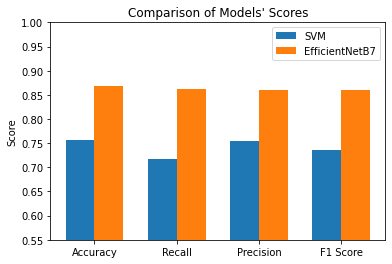
\includegraphics[width=9cm]{charts/EfficientNetB7_VS_SVM.png}
        \caption[Comparison between EfficientNet-B7 and SVM]{Comparison between best cnn model and best SVM model.}
        \label{fig:EfficientNetB7VsSVM}
    \end{figure} 

    \newpage
    \section{Conclusion}
    \hspace{0.7cm} As research has recently gravitated toward DL algorithms for image recognition, the automated detection of skin cancer using these DL algorithms can be used by patients and physicians to more easily and accurately diagnose skin cancer. 
    The majority of the papers we found in the field of skin cancer detection focused on applying DL algorithms to improve the process of detecting skin cancer since it yields promising results quickly, and it is an expensive and difficult process if the patient does it without automation. Moreover, we discovered a dearth of research focusing on shallow learning algorithms. In contrast, models created using DL were common. DL can serve as a standard for skin cancer detection by assisting medical professionals.
    In the field of skin cancer detection, there are currently few large datasets for skin cancer imaging that can be used for supervised learning, which is the reason for the interest and application of data augmentation in prior work.
    In this research, we tackled the problem of detecting skin cancer by segmenting the tumors from skin lesions in the images using U-Net, generating more images to deal with the lack of large datasets using GAN,  implementing the pre-trained CNN models: ResNetV2, VGG16, EfficientNet B5, and EfficientNet B7, and compared their performance with SVM. After presenting and analyzing the models’ performance, we found that EfficientNet-B7 has the highest accuracy which is 86.91\%. 
    Our study showed that image augmentation using GAN models can help complex DL models' accuracy in detecting malignant skin lesions, it also highlights the need for larger and more diverse datasets to further improve the performance of DL algorithms in this domain. Future research should focus on addressing these limitations and explore the potential of other DL techniques, such as attention-based models, to improve skin cancer detection. Additionally, there is a need to conduct clinical studies to evaluate the real-world effectiveness of these algorithms and their impact on patient outcomes. Overall, we believe that continued research in this area has the potential to make a significant impact on the field of dermatology and ultimately improve patient care.


    \newpage
    \bibliographystyle{ieeetr}
    \bibliography{citation.bib}

\end{document}